%%%%%%%%%%%%%%%%%%%%%%%%%%%%%%%%%%%%%%%%%%%%%%%%%%%%%%%%%%%%%%%%%%%%%%%%%%%%%%%%
% \documentclass[12pt,papel,twoside]{ibtesis}
%\documentclass[12pt,screen,twoside,pagebackref]{ibtesis}
 \documentclass[12pt,papel,singlespace,oneside]{ibtesis}
% \documentclass[12pt,papel,preprint,singlespace,oneside]{ibtesis}
%%%%%%%%%%%%%%%%%%%%% Paquetes extra %%%%%%%%%%%%%%%%%%%%%%%%%%%%%%%%%%%%%%%%%%%
% Por conveniencia: aqu\'{\i} puede cargar todos los paquetes y definir los comandos 
% que necesite
\usepackage{ibextra}
\usepackage{subfig} %para poner varias imagenes en una sola figura
\usepackage{url} %para citar páginas web
\usepackage{notoccite}
\usepackage{verbatim} 
%\nofiles
%%%%%%%%%%%%%%%%%%%%%%%%%%%%%%%%%%%%%%%%%%%%%%%%%%%%%%%%%%%%%%%%%%%%%%%%%%%%%%%%
%%%%%%%%%%%%%%%%%%%%% Informacion sobre la tesis %%%%%%%%%%%%%%%%%%%%%%%%%%%%%%%
\title{FILMS DE MgB$_2$: POSIBILIDAD DE USO COMO DETECTOR DE NEUTRONES}
\author{Lic. Emanuel Alejandro Benatti}
\director{Dr. Mariano Gómez Berisso}
\carrera{Tesis Carrera de Maestría en Ciencias F\'{\i}sicas}
\grado{Maestrando}
\laboratorio{Laboratorio de Bajas Temperaturas -- Centro At\'{o}mico Bariloche}
\jurado{Dr.~H.~Pastoriza (Centro Atómico Bariloche - Instituto Balseiro) \\ 
Dr.~J. Luzuriaga (Centro Atómico Bariloche - Instituto Balseiro)\\ 
Dr.~J.~Blostein (Centro Atómico Bariloche - Instituto Balseiro)}
\palabrasclave{DETECTOR, SUPERCONDUCTOR, MgB$_{2}$, NEUTRÓN}
%\keywords{detector, superconductor, MgB$_{2}$, neutron}
% Si queremos poner la fecha manualmente:
% \date{Diciembre de 2099}

%%%%%%%%%%%%%%%%%%%%%%%%%%%%%%%%%%%%%%%%%%%%%%%%%%%%%%%%%%%%%%%%%%%%%%%%%%%%%%%%
\titlepagefalse % Si no quiere compilar la portada descomente esta linea
%\includeonly{apendices} % Compilar s\'{o}lo estos archivos 
%\graphicspath{{figs/}} % Lugar donde encontrar las figuras generales (se puede poner uno en cada cap{\'{\i}}tulo)
%%%%%%%%%%%%%%%%%%%%%%%%%%%%%%%%%%%%%%%%%%%%%%%%%%%%%%%%%%%%%%%%%%%%%%%%%%%%%%%%


\begin{document}

% Dentro del environment 'preliminary' va:
% la dedicatoria, resumen, abstract, indices

\begin{preliminary}

% Escriba su dedicatoria
\dedicatoria{
A mi familia\\
A mis amigos\\
y a todos aquellos cronopios, famas y esperanzas \\
que me han permitido llegar hasta aquí
}

%%% \'{I}ndices %%%%
%\begin{abreviaturas}
%\printnomenclature
%\end{abreviaturas}

\tableofcontents                %\'{I}ndice

%\listoffigures                  %Figuras

%\listoftables                   %Tablas

%\listofabbr						%Símbolos y abreviaturas

\begin{resumen}%
  En este trabajo se estudia la viabilidad de utilizar films del supuerconductor MgB$_2$, que tiene una temperatura crítica alrededor de 39\,K, para construir un detector de neutrones térmicos y fríos. El objetivo es aprovechar el calor generado por la reacción $^{10}$B$(n,\alpha)^6$Li que tiene una sección eficaz de 3800\,barns para neutrones térmicos y libera una energía de aproximadamente 2.3\,MeV. El calor producido por la reacción produce una supresión momentánea de la superconductividad, lo que produce una señal que permite registrar la captura de un neutrón. Se realizaron simulaciones de las trayectorias de los productos de la reacción en el MgB$_2$ para estimar las dimensiones del detector que permitan maximizar su señal, sensibilidad y eficiencia, y que minimicen el tiempo de respuesta, al tiempo que se estimó que la energía de la reacción se deposita en un volumen de unos pocos micrómetros cúbicos. Cálculos y simulaciones hechas con el software comercial de elementos finitos COMSOL MULTIPHYSICS llevaron a la conclusión de que para poder detectar eficientemente neutrones con el MgB$_2$, resulta necesario construir un cable que tenga un ancho no mayor a un micrón y un espesor no mucho mayor a los 200\,nm. Dimensiones mayores incrementan la probabilidad de captura de un neutrón pero reducen drásticamente la señal y la sensibilidad del detector, además de que dificultan el control de la temperatura del mismo.

Fueron realizadas simulaciones en las que se acopló la física del comportamiento térmico y eléctrico del detector, y se observó que si el mismo es operado con corrientes lo suficientemente bajas, la señal y el tiempo de respuesta del detector no se modifican, y que tiene un tiempo de respuesta de algunos nanosegundos cuando el espesor del cable es de 200\,nm. También se llevaron a cabo simulaciones intentando regular la temperatura del detector simplemente variando la tensión aplicada al mismo, pero el resultado fue que eso no es posible desde el punto de vista práctico, ya que para regular la temperatura del detector en el rango de interés, es preciso aplicar tensiones que llevan a que circulen corrientes enormes por el cable de MgB$_2$. La conclusión extraída de este cálculo fue que el detector va a requerir un mecanismo adicional para controlar su temperatura. También se concluyó que por razones de estabilidad en el control de la misma, es conveniente operar al detector a tensión constante, en vez de hacerlo a corriente constante.

En conjunto con el trabajo de las simulaciones se intentó crecer films de MgB$_2$ por medio de dos técnicas diferentes, una utilizando un método ex-situ que requrió temperaturas del orden de los 700\,$^{\circ}$C, y otra consistente en un método in-situ que requería temperaturas iban de los de 500\,$^{\circ}$C hasta temperatura ambiente.

La primera técnica de crecimiento consistió en depositar films de B por evaporación para luego recocer los mismos junto con pastillas de MgB$_2$ bulk en ampollas de cuarzo. Se lograron fabricar films de un espesor de algunos cientos de nanómetros, cuyas curvas de magnetización, medidas en un magnetómetro SQUID, presentaron irreversibilidades en un ciclo \textit{Zero Field Cooling - Field Cooling} compatibles con la formación de una fase superconductora. Sin embargo, siguiendo este método no se pudo conseguir fabricar films con una transición superconductora lo suficientemente estrecha como para poder fabricar el detector, lo que probablemente se debió a que el sustrato reaccionaba con el film debido a las elevadas temperaturas del recocido.

La segunda técnica de crecimiento de films de MgB$_2$ explorada en este trabajo fue la de crecimiento directo de films por sputtering, a partir de un blanco de MgB$_2$ obtenido comercialmente. Se realizaron estudios de difracción de rayos X que no mostraron la formación de la fase MgB$_2$. Un estudio de la composición de los films crecidos fue realizado utlizando espectroscopía de rayos X caracterísiticos (EDX) y retrodispersión de Rutherford (RBS). Ambos estudios mostraron que los films crecidos tienen un exceso de B, lo que probablemente sea la causa de que no sean superconductores, tal como mostraron las mediciones de magnetización realizadas sobre las muestras. Se decidió intentar recocer los films crecidos con pastillas de Mg, en busca de mejorar la proporcion B/Mg de los films utilizando una temperatura de recocido más baja que la empleada con los films crecidos por evaporación. El recocido logró una mejora en las propiedades de transporte de las muestras, ya que pasaron de ser aislantes a ser semiconductoras, pero no se pudo observar la formación de fases superconductoras, ni en mediciones de magnetización, ni en mediciones de transporte, lo que consituye un indicio de que los films no lograron incorporar la cantidad suficiente de Mg como para volverse superconductores. Esto último se deba probablemente a que la temperatura de recocido no fue lo suficientemente alta como para permitir la difusión de la cantidad necesaria de Mg a través del film.
\end{resumen}

\begin{abstract}%
	In this paper we study the feasibility of using films of the superconductor MgB$_2$ with a critical temperature of 39\,K, to build a cold neutron and thermal neutron detector. The aim is to use the heat generated by the reaction $^{10}$B$(n,\alpha)^6$Li which has a cross section of 3800\,barns for thermal neutrons and releases an energy of approximately 2.3\,MeV. The heat produced by the reaction causes a partial destruction of superconductivity. One then notices the appearance of a single neutron by the electric resistance variation of the MgB2 thin film. Simulations of the trajectories of the reaction products in the MgB$_2$ were performed for estimating the optimal detector dimensions. Calculations and simulations with the commercial software COMSOL Multiphysics led to the conclusion that in order to efficiently detect neutrons with MgB$_2$, is necessary to build a cable that has a width no greater than one micron and a thickness not much greater than 200\,nm. Larger dimensions increase the probability of neutron capture but drastically reduces the produced signal and the detector sensitivity, plus it difficult the temperature control of the device.

	Simulations were also conducted coupling the physics of the thermal and electrical behavior of the detector, and it was found that if it is operated with a small bias-current, the detector's signal and response time are not changed. Calculations showed that the detector has a response time of few nanoseconds for a wire 200\,nm thick. Simulations were carried out trying to regulate the temperature of the detector by varying the bias tension, but it was found that this is not a viable option from a practical standpoint, as to regulate the temperature of the detector in the range of interest, it is necesary to apply voltages that lead to large currents circulating through the detector. This implied that the construction of the detector will require an additional mechanism to control its temperature. It was also found that for reasons of stability in temperature control, it is desirable to operate the detector voltage-biased instead of current-biased.

	In addition with the simulations, growth of MgB$_2$ films was attempted by two different means, one using an ex-situ method requiring temperatures around 700\,$^{\circ}$C, and an in-situ method requiring temperatures of 500\,$^{\circ}$C down to room temperature.

	The first technique consisted on growing of boron films by evaporation and a post-annealing process with a bulk MgB$_2$ sample in a quartz tube. We managed to make 200\,nm thick films, and perform magnetization measurements in a SQUID magnetoteter. Irreversibilities shown in a Zero Field Coolig - Field Coolig magnetization measurement were compatible with the formation of a superconducting phase. However, it wasn't possible to obtain films with a sharp superconducting transition, as it's needed to build the detector. This is probably the result of a chemical reaction between substrate and the film due to the high annealing temperatures.

  The second technique explored in this work was the direct growth of MgB$_2$ films by sputtering. To this end a commercial MgB$_2$ target was used. Studies performed by X-ray diffraction did not show the formation of the MgB$_2$ crystalline phase. We also studied the composition of the films by electron dispersive X-ray analisys (EDX) and Rutherford backscattering (RBS). Both studies showed that films are grown with an excess of B, which is probably the reason why they are not superconducting, as was observed by magnetization measurements. Films were annealed with Mg pellets, seeking to increase the amount of Mg in the films, using lower annealing temperatures than those used with the films grown by evaporation. Samples showed an improvement in their transport properties after the annealing, as they went from being insulating to semiconductonducting. However no formation of a superconducting phase was observed, neither in magnetization measurements or in electrical resistance measurements. This is probably due to the low annealing temperature, which did not allow the diffusion of the required amount of Mg through the film.
\end{abstract}

%%% Local Variables: 
%%% mode: latex
%%% TeX-master: "template"
%%% End: 

\end{preliminary}


% Podemos usar cualquiera de los dos comandos: \input o \include para incluir el texto
\chapter{Introducci\'on}
\graphicspath{{./figs/01_intro/}}
\chapterquote{La destrucción es obra de una tarde. La creación es obra de una vida.}{Kamahl, acólito druida}
\section{Motivación}\label{S:motivacion}
\cite{Mainprice2011}
\section{Difracción de Rayos X}\label{S:DRX}
Los rayos X son una herramienta de vital importancia para el estudio de los materiales cristalinos. 
En la difracción de Rayos X (DRX), un haz monocromático de de rayos X de longitud de onda $\lambda$ incide sobre una dada muestra (Fig. \ref{fig:Bragg}). 
Si el cristal es infinito y está libre de cualquier tipo de distorsiones, para una dada familia de planos ${hkl}$, habrá interferencia constructiva para los haces salientes que cumplan con la condición de Bragg[ref]:

Esto esta medio medio, hay que hablar de que los cristales estan en arreglos periodicos de atomos

\begin{equation}
  2 \ d_{hkl} \ \sin(\theta_{B}) \ = \ n \ \lambda
  \label{eq:Bragg}
\end{equation}
\noindent
siendo $d_{hkl}$ la distancia interplanar de la familia de planos $\{hkl\}$, 2$\theta_{B}$ el ángulo formado entre el haz incidente y el haz reflejado y $n$ el número de orden de difracción. 

Hay que pensar en el planteo mas riguroso, usando los vectores K, porque lo voy a necesitar para explicar williamson hall

\nomenclature{$\lambda$}{Longitud de onda}
\nomenclature{$d_{hkl}$}{Distacia interplanar para la familia de planos $hkl$}
\nomenclature{$\theta_B$}{Ángulo de Bragg}
\nomenclature{XRD}{Difracción de Rayos X}
\begin{figure}[htb!]
  \centering
  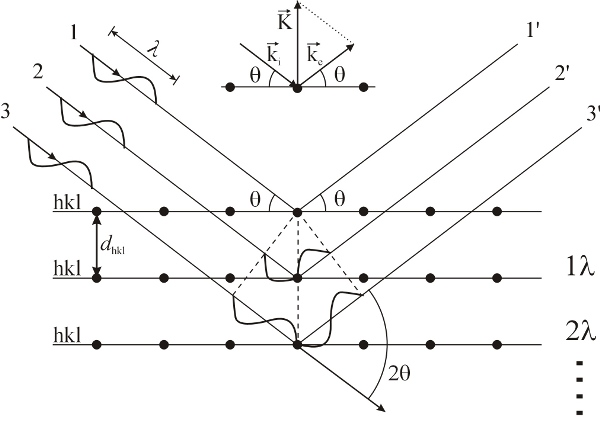
\includegraphics[width=\imsize]{BraggLaw}
  \caption{Ley de Bragg}
  \label{fig:Bragg}
\end{figure}

Una consecuencia de la ley expresada en la Ec. \ref{eq:Bragg} es que para un cierto haz incidente habrá reflexiones cuyas distribución de intensidades serán funciones deltas de Dirac[ref], con intensidad infinita para el ángulo $\theta_{B}$ e intensidad nula para los ángulos $\theta$ que no cumplan con la condición de Bragg. Como resultado, los "picos" de difracción tendrán además un ancho nulo. 
Si, como ocurre en la práctica, el número de planos que contribuyen a la reflexión es finito, la distribución angular de intensidades tendrán un ancho y altura finitos, y lo mismo ocurrirá si la red de átomos tiene distorsiones, es decir, si los átomos no se encuentran en un arreglo perfectamente periódico. 
En un experimento de DRX real aparecerán además otras contribuciones que ensancharán los picos de difracción. 
Por un lado el haz incidente no será puntual ni estará constituido por haces completamente paralelos, sino que tendrá de un tamaño finito y estará comprendido entre haces que tendrán cierta divergencia angular. 
Además, el haz no será completamente monocromático, sino que estará inegrado por rayos X con longitudes de onda en un intervalo $(\lambda \ \pm \ \Delta \lambda)$. 
Todos estos factores cotribuirán a que haya haces difractados en las vecindades de $\theta_{B}$, aumentando el ancho de los picos de difracción, y serán parte crucial de la discusión en los capítulos siguientes, ya que el ensanchamiento de los picos provee información sobre la microestructura de los materiales.

\subsection{Estudios de ancho de pico}\label{SS:DRX-LPA}
Si no se tienen en cuenta los diferentes efectos instrumentales se puede afirmar que, a partir del estudio del ensanchamiento y la forma de los perfiles de intensidad de los picos de medidos en un experimento de DRX, es posible obtener información acerca de la cantidad y tipo de defectos presentes en un material, así como información microestructural como el tamaño promedio de los dominios coherentes de difracción. 
Al conjunto de t\'ecnicas y m\'etodos del campo de la cristalografía que utilizados para obtener este tipo de información se los conoce como Estudio de Ancho de Pico, o LPA, por sus siglas en inglés (Line Profile Analysis).
Aunque el término LPA fue acuñado muchos años después, la técnica, aunque rudimentaria, es tan antigua como los primeros experimentos de DRX, y fue implementada independientemente por Hull en Estados Unidos y Debye y Scherrer en Alemania. Mientras investigaba el tamaño de partículas de oro y plata en sistemas coloidales, Scherrer incluyó la ecuación que luego llevaría su nombre[ref]:

\begin{equation}
  H \ = \ 2 \sqrt{\frac{\ln(2)}{\pi}} \ \frac{\lambda}{L \ \cos(\theta_B)}
  \label{eq:Scherrer}
\end{equation}
\noindent
Donde $H$ denota el ancho del pico a la mitad de su intensidad máxima, $L$ es la longitud característica de la cristalita y el factor numérico se usa para convertir $H$ al ancho integral del pico, suponiendo que el mismo tiene forma de gaussiana. 
Los trabajos que siguieron se dedicaron a mejorar las estimaciones de tamaño y forma de las cristalitas. 
En el año 1938 [ref] Jones señaló que el perfil de intensidades medido en un experimento de DRX, $I_{exp}$ es la convolución del perfil $I_{muestra}$ que se obtendría de la muestra y el debido a todos los efectos instrumentales, $I_{inst}$, es decir:
\begin{equation}
  I_{exp} \ = \ I_{muestra} \ \otimes \ I_{inst}
  \label{eq:conv}
\end{equation}
\noindent
De esta manera, Jones logró remover las contribuciones de las líneas $K\alpha_2$ de la radiación del cobre en las mediciones de tamaño de cristalita.


\nomenclature{$H$ o $FWHM$}{Ancho de pico a media altura. También abreviado como FWHM por sus siglas en inglés (Full Witdth at Half Maximum).}
\nomenclature{$L$}{Longitud característica de la cristalita.}

Frase de Warren?
Definicion de macro, micro, meso, nano estructura?
Diferencia entre cristalita y tamaño de grano
Definicion de defectos, dislocaciones, maclas, fallas de apilamiento, bordes de grano
Separacion, al menos en la nomenclatura de familia de planos, planos, direcciones familia de direcciones

Hay que hablar de los principios de medicion, rayos X de laboratorio y de sincrotron
Estudio de ancho de pico, Langford, Williamson Hall, Warren Averbach y CMWP

\section{Difracción de electrones retro difundidos}\label{S:EBSD}
Cómo se mide y cómo se pueden relacionar las magnitudes de EBSD con las de RX
Que permite y que no permite ver en comparacion con RX

¿Hablo de TEM?
 
\section{Textura cristalográfica}\label{S:Text}
Definicion de textura, relacion con los procesos de deformacion y la microestructura.
ODF: definicion y obtencion a partir de RX y EBSD. Diferencias de los dos métodos.

\subsection{FDO y FDO generalizada}\label{SS:ODF}
Relacion entre la ODF y la ODF generalizada. Relacion de FWHM y energía de deformacion.

\section{Revisión bibliográfica y estado del arte}\label{S:RB}

\section{Organización de la tesis}\label{S:Org}

%\chapter{Diseño del detector}\label{C:dise}
\graphicspath{{figs/dise/}}

\chapterquote{The only action worth taking is the one with an unknown outcome}{Anónimo}
%%%%%%%%%%%%%%%%%%%%%%%%%%%%%%%%%%%%%%%%%%%%%%%%%%%%%%%%%%%%%%%%%%%%%%%%
En este capítulo se estudian los aspectos que hacen al diseño del detector, así como a su sensibilidad, resolución espacial, eficiencia, tiempo de respuesta y señal producida ante el evento de la captura de un neutrón. Cada uno de estos aspectos se encuentran íntima y a veces contradictoriamente relacionados. Por ejemplo, si se quiere incrementar la eficiencia de un detector, es necesario incrementar el volumen disponible para la detección, lo que en general redunda en un detrimento de la resolución espacial del detector. Estos aspectos condicionan a su vez el diseño físico del detector, su geometría y la electrónica asociada que permite la lectura de los eventos, por lo que conocer a priori el diseño que optimiza el desempeño del detector ante la aplicación requerida puede resultar en un gran ahorro de tiempo, esfuerzo y dinero.

En la primer parte del capítulo (sección \ref{S:term}) se hace un cálculo del volumen en que se deposita la energía de la reacción nuclear, realizando simulaciones que permiten calcular el rango en MgB$_{2}$ de los iones que se producen en la fisión del B. Con este dato se simula, utilizando el método de elementos finitos, el calentamiento y enfriamiento de un cable de MgB$_{2}$ que se encuentra en condiciones parecidas a las de operación del detector, a partir de lo cual se hace una estimación del tiempo de respuesta del detector. Paralelamente, y con la misma estimación del volumen en que se deposita la energía de la reacción, se calcula el cambio de la resistencia del mismo cable de MgB$_{2}$ al incrementarse la temperatura del mismo gracias al calor generado por la fisión del $^{10}B$, lo que da una medida de la señal que se puede obtener como resultado de la captura de un neutrón. Tanto el análisis térmico como el eléctrico se realizan variando la geometría del cable de MgB$_{2}$. Este trabajo se desarrolla en las secciones \ref{S:term} y \ref{S:signal}.

En la sección \ref{S:termyelec} se acoplan los dos elementos estudiados en las secciones an\-te\-rio\-res, es decir, el cálculo de la señal y el tiempo de relajación del sistema, incorporando el efecto Joule como mecanismo de generación de calor adicional a la reacción nuclear. Cabe mencionar que aunque estos aspectos pueden parecer débilmente acoplados, la fuerte no linealidad que tiene la resistividad del MgB$_{2}$ en la transición superconductora, resulta finalmente en la existencia de una fuerte interacción, lo que redunda en numerosas dificultades a la hora de calcular una solución. En esta misma sección se hace una revisión de los resultados obtenidos en las secciones \ref{S:term} y \ref{S:signal}. Finalmente, en
\newpage
\noindent
la sección \ref{S:eficiencia} se estudia la eficiencia esperada del detector en función de su geometría y proporción de $^{10}$B.
\section{Respuesta térmica del detector}\label{S:term}
El funcionamiento del detector consiste en utilizar la energía de las partículas creadas por la reacción de captura de un neutrón por un núcleo de $^{10}$B, que se fisiona en un átomo de $^4$He y otro de $^7$Li. Dichos átomos depositan su energía cinética en el MgB$_2$, incrementando su temperatura, lo que produce una supresión momentánea de la superconductividad. Teniendo en cuenta esto, resulta evidente que el detector no será capaz de distinguir la llegada de dos neutrones que lleguen con una separación temporal menor que $\tau$, el tiempo que le tome al superconductor retornar a su tem\-pe\-ra\-tu\-ra inicial. De ahí que la determinación del tiempo de relajación $\tau$ (también lla\-ma\-do tiempo de respuesta) del detector, sea un factor crucial en la construcción del mismo, ya que permite determinar la electrónica más adecuada para operarlo, y el máximo flujo de neutrones para el que se tiene resolución individual de partículas detectadas.


El primer paso para conocer la respuesta térmica del detector, consiste en estimar el volumen en que las partículas creadas por la reacción nuclear depositan su energía. Utilizando el software SRIM-2008 se simularon las trayectorias de las partículas producidas por la reacción $^{10}\text{B}(n,\alpha)^{7}\text{Li}$, utilizando consideraciones dinámicas clásicas para deducir la energía cinética inicial de cada uno de los productos. Si se desprecia la velocidad inicial del neutrón (que tiene una energía del orden de las décimas de eV, mientras que el $Q$ de la reacción es del orden de los MeV), la conservación del impulso dice que la energía cinética inicial de la partícula $\alpha$ es de 1.464\,MeV y la del Li es de 0.836\,MeV. 
\begin{figure}[h!]
 \centering
 \subfloat[He en MgB$_2$]{\label{h01}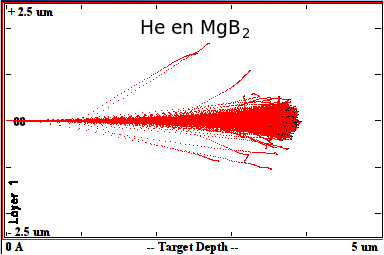
\includegraphics[width=0.5\columnwidth]{Hexy}}\hspace{0.1cm}
 \subfloat[Li en MgB$_2$]{\label{h02}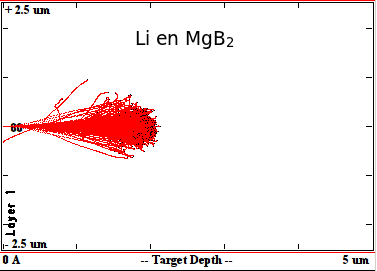
\includegraphics[height=5cm]{Lixy}}
   \caption[Dispersión de iones de He (\ref{h01}) y Li (\ref{h02}) en MgB$_2$]{Dispersión de iones de He (\ref{h01}) y Li (\ref{h02}) en MgB$_2$. Se simuló la colisión de cada uno de los iones en un medio semi infinito de MgB$_2$. A partir de estas simulaciones se estimó que las partículas producidas por la reacción $^{10}\text{B}(n,\alpha)^{7}\text{Li}$ depositan su energía en un volumen $V \, = \, 2.48 \, \mu$m$^3$.}
\label{fig:HeLixy}
\end{figure}

En la Fig.\,\ref{fig:HeLixy} se ven las trayectorias simuladas para cada ion. Los mismos incidían sobre un medio semi-infinito de MgB$_2$ de densidad 2.62\,g/cm$^{3}$\cite{Lui2003}. Esto sería similar a pensar que los productos de la fisión salen en dirección paralela al cable de MgB$_2$. Como el rango de las partículas en el MgB$_2$ es alrededor de 4\,$\mu$m para el He y 2\,$\mu$m para el Li, una conclusión inicial que se puede extraer es que si las partículas salen en dirección perpendicular al cable, la energía depositada en el mismo será muy pequeña, salvo que el ancho y el espesor del cable sean comparables con el rango del He y el Li en MgB$_2$. Sin embargo, más adelante se verá que debido a la dinámica térmica del sistema, el cable de MgB$_2$ debe tener un espesor y un ancho del orden del micrón, ya que de otro modo la señal y la sensibilidad del detector disminuyen drásticamente.

Como primera aproximación al problema se consideró que toda la energía de las partículas se deposita en un único volumen $V_{hs} \, = \, 2.48 \, \mu$m$^3$, y luego se calculó el incremento de temperatura $\Delta T$ que sufre ese volumen de MgB$_2$ como consecuencia de la captura de un neutrón y la reacción nuclear siguiente:
\begin{equation}
  \Delta T \ = \ \frac{Q}{c_p\,V_{hs}\, \delta} \ \approx \ 3.5 \, K
  \label{eq:DT}
\end{equation}
\noindent
donde $Q = 2.3$\,MeV\cite{Nishikawa2008} es la energía liberada en la reacción de captura de un neutrón, $\delta$ es la densidad del MgB$_2$ \cite{Lui2003} y $c_p \ = \ 17$\,J/(kg K) es su calor específico a presión constante \cite{Putti2003} a una temperatura de 39\,K.

La evolución temporal de la temperatura se estudió utilizando un software comercial de simulación por medio del método de elementos finitos (COMSOL MULTIPHYSICS). Se simuló la evolución térmica a lo largo del tiempo de un alambre de MgB$_2$ de 2\,$\mu$m de ancho y con distintos espesores entre 0.2\,$\mu$m y 1.8\,$\mu$m. Se consideró que el mismo se encuentra depositado sobre un sustrato de Si o zafiro de 2\,$\mu$m de espesor, 4\,$\mu$m de ancho y largo igual al del alambre. Los valores de conductividad térmica y calor específico del MgB$_2$ se obtuvieron de \cite{Putti2003} y \cite{Bauer2001}, respectivamente. Los datos análogos del Si se obtuvieron de \cite{Flubacher1959} y de las librerías de propiedades físicas del software COMSOL MULTIPHYSICS. Las propiedades físicas del zafiro también se obtuvieron de las bibliotecas de propiedades del programa COMSOL. En el apéndice \ref{C:tablas} se muestran los datos de entrada empleados en la realización de todas las simulaciones de este trabajo.
\begin{figure}[tbh!]
 \begin{center}
    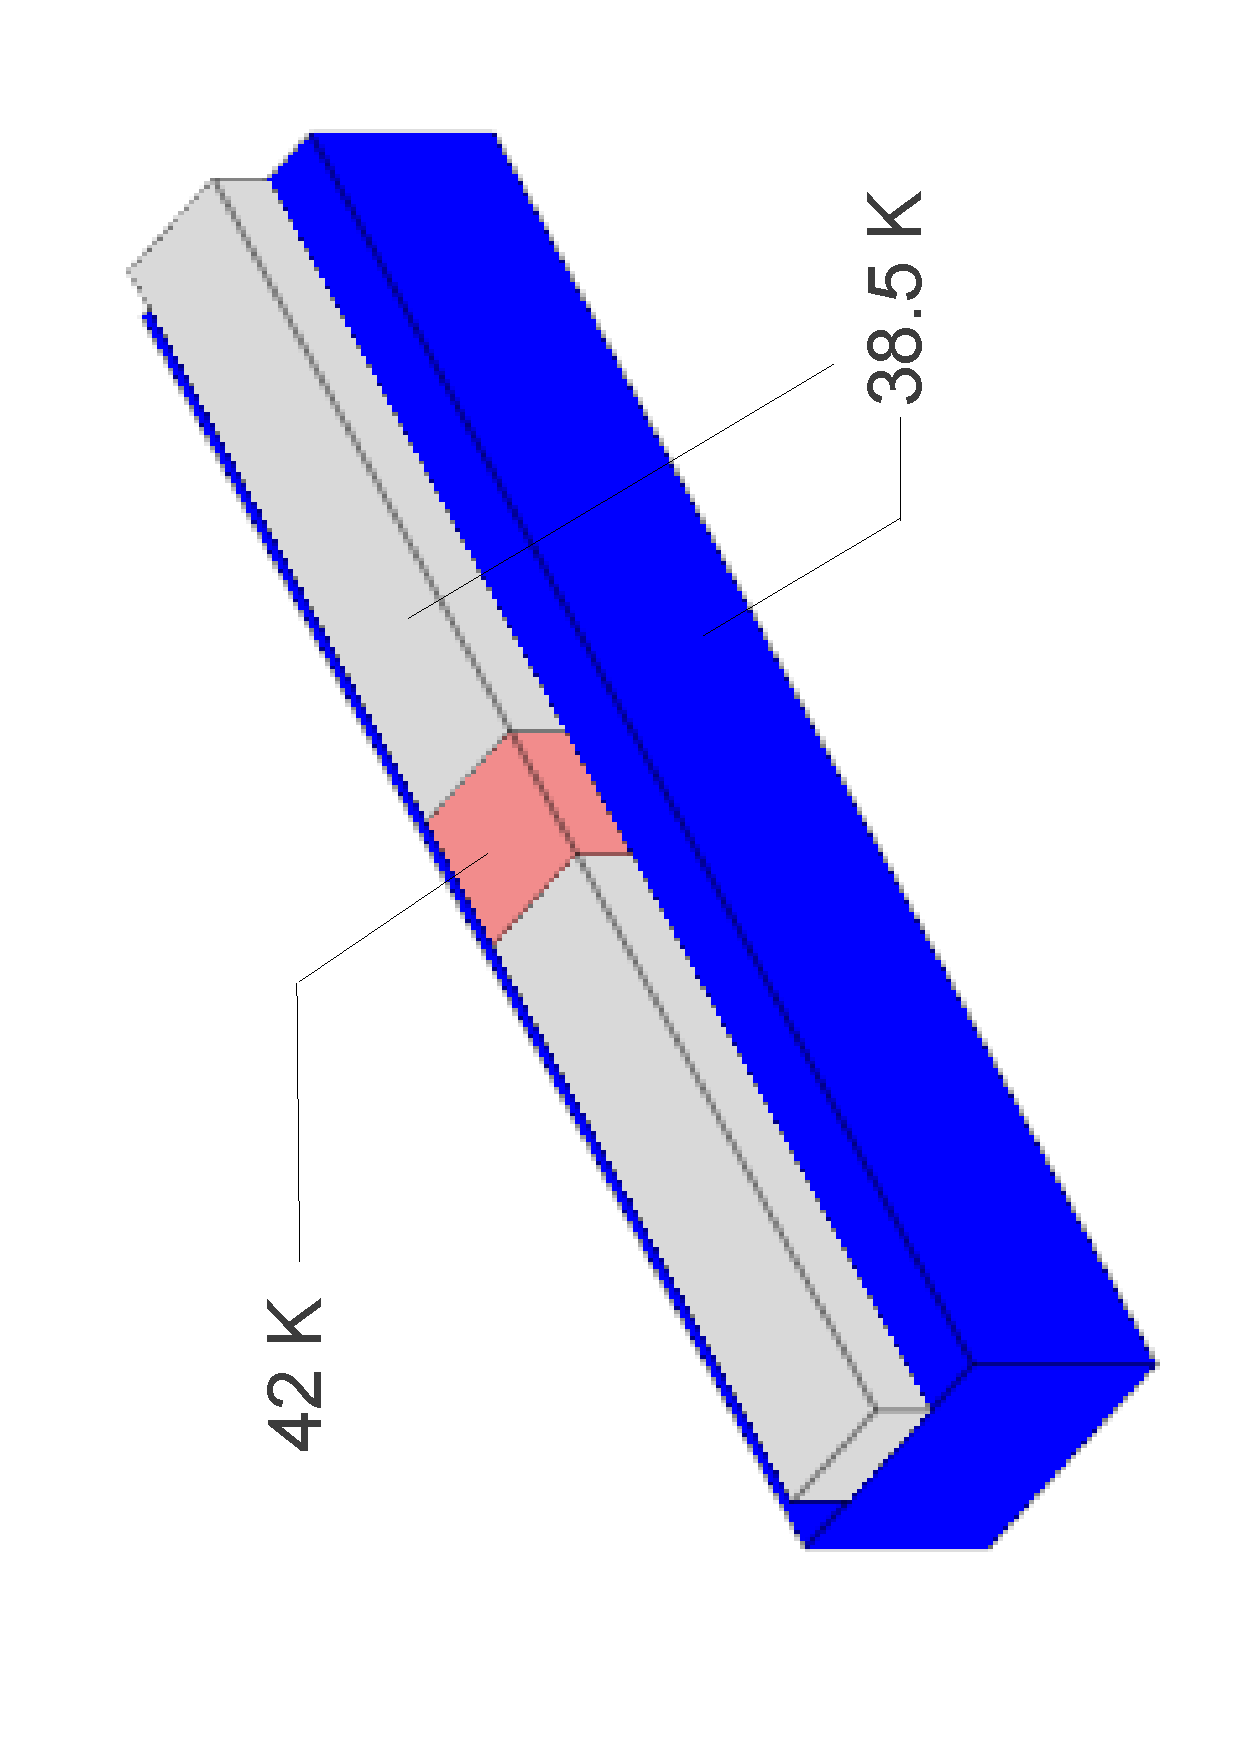
\includegraphics[width=0.45\columnwidth, angle=-90]{sim}
  \end{center}
  \caption[Condiciones de borde utilizadas para simular el comportamiento térmico de un cable de MgB$_2$.]{Se realizó una simulación que consistió en un alambre de MgB$_2$ (gris y rosa) depositado sobre un sustrato que era de silicio o zafiro (azul). Se consideró como condición inicial que todo el sistema estaba a una temperatura de 38.5\,K salvo una porción de 2.48\,$\mu$m$^3$ de volumen (rosa), que se encontraba a 42\,K. Se consideró que la tapa inferior del sustrato se mantenía a temperatura constante e igual a 38.5\,K. El resto del sistema se consideró térmicamente aislado.}
\label{fig:bordes}
\end{figure}

Se consideró una temperatura de operación $T_o \, = \, 38.5$\,K, correspondiente al flanco de la transición superconductora del MgB$_2$\cite{Nagamatsu2001}. Se supuso que el calor se deposita en un volumen $V_{hs}$ y la forma de este volumen cambió de modo que pudiera caber en el alambre (esto es, el volumen se iba haciendo más corto a medida que su espesor aumentaba). Se consideró este criterio con el fin de comparar la variación del tiempo de respuesta del detector para cables de diferentes geometrías que sufren el mismo incremento de temperatura. Un análisis posterior a este tipo de simulaciones mostró que el tiempo de respuesta no se afecta notablemente con la forma y el tamaño que se le asigne a $V_{hs}$. El sistema era lo suficientemente largo como para despreciar cualquier efecto de borde que pudiera aparecer y la condición inicial fue que todo el sistema estaba una temperatura $T_o$, salvo el volumen $V_{hs}$ que tenía una temperatura inicial $T_h \, = \, T_o\, + \, \Delta T$ (Fig.\,\ref{fig:bordes}).

Las condiciones de contorno se impusieron analizando el ambiente de operación del detector. La cara inferior del sustrato fue mantenido a temperatura constante e igual a $T_o$ y se consideró que el resto de las caras estaban aisladas térmicamente del exterior. Esto se hizo así porque el detector va a operar en condiciones de vacío (lo que elimina pérdidas por conducción y convección). Las pérdidas por radiación máximas fueron estimadas a partir de la ecuación de Stefan-Boltzmann\cite{incropera}:
\begin{equation}
\dot{q} \ = \ A\,\sigma \ (T_{detector}^4 \, - \, T_{amb}^4)
\label{eq:sb}
\end{equation}
\noindent
con $\dot{q}$ el flujo saliente de calor, $A$ el área expuesta, $\sigma$ la constante de Stefan-Boltzmann, $T$ la temperatura del detector y $T_{amb}$ la temperatura del medio exterior (considerada como la temperatura de nitrógeno líquido). El flujo de calor por radiación fue comparado con el flujo de calor que existe por conducción a través del MgB$_2$ y del sustrato. Se vio que el flujo de calor por radiación es menor que el flujo por conducción en un factor $10^{7}$, de donde se concluyó que el sistema está térmicamente aislado. Si la temperatura exterior es la ambiente las pérdidas por radiación son menores en un factor $10^{4}$.
\begin{figure}[t!]
 \begin{center}
    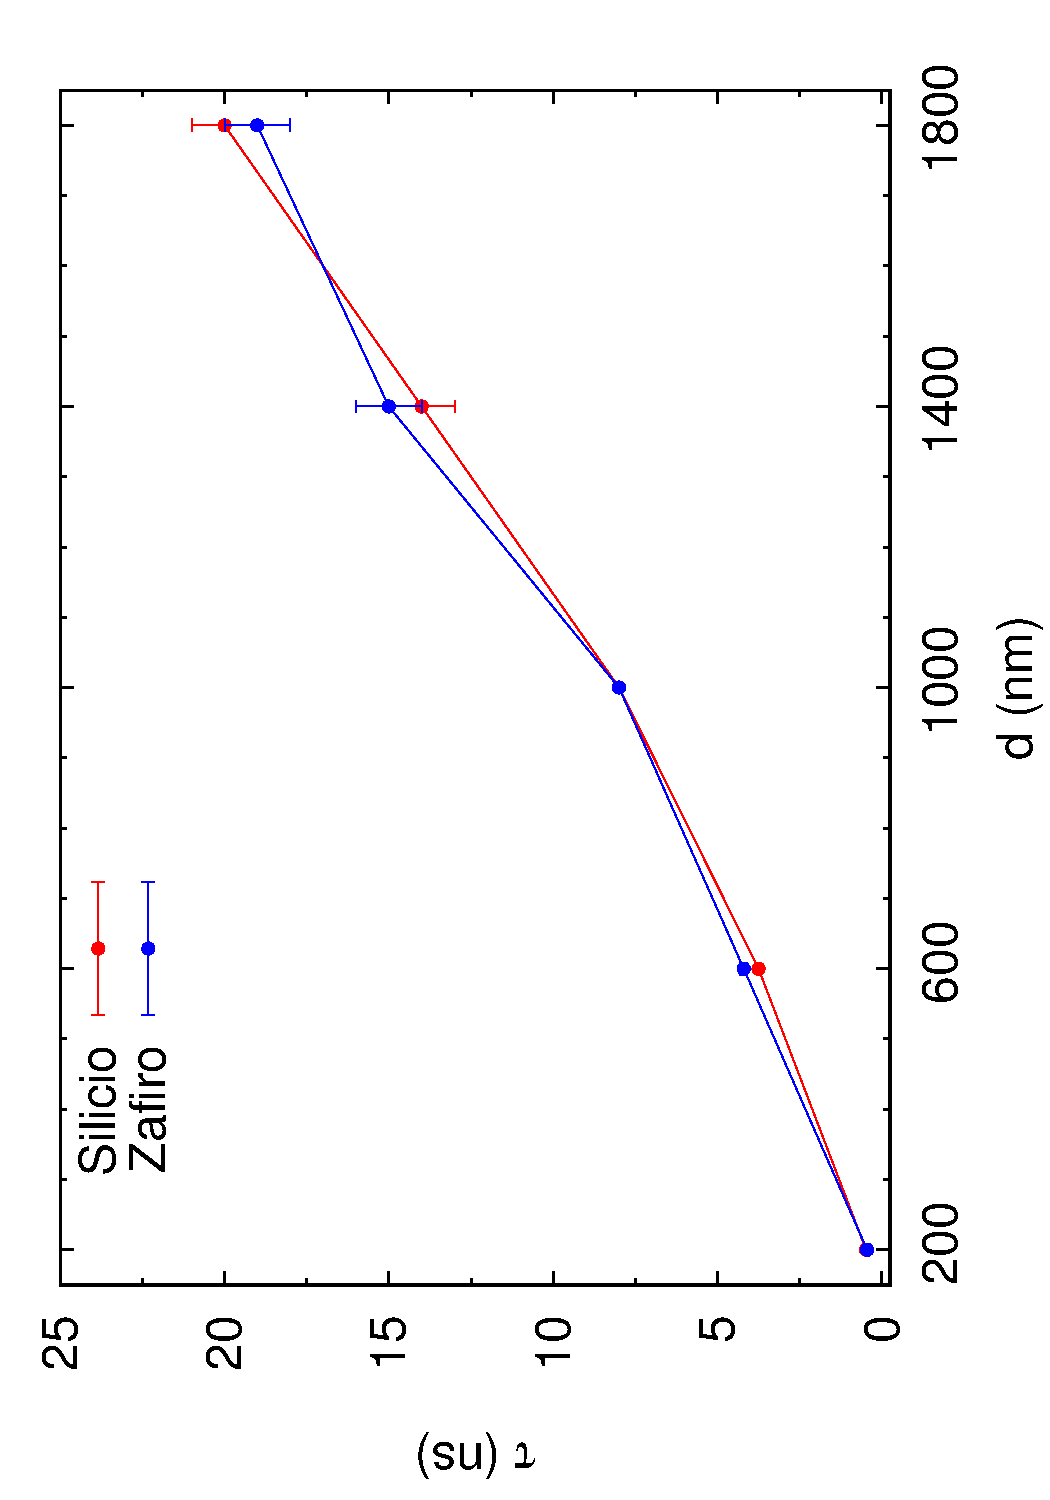
\includegraphics[width=0.55\columnwidth,angle=-90]{tau}
 \end{center}
  \caption[Tiempo de relajación de un cable de MgB$_2$ para diferentes sustratos.]{Tiempo de relajación $\tau$ en función del espesor $d$ de un alambre de MgB$_2$ para diferentes sustratos. Se
concluye de observar la figura que el tiempo de res\-pues\-ta del sistema varía de los pocos nanosegundos a algunas decenas de
nanosegundos para espesores del orden de micrón y que $\tau$ es prácticamente independiente del sustrato utilizado.}
\label{fig:tau}
\end{figure}

Considerando todos estos factores se estudió la evolución temporal de la temperatura del detector y se estimó la variación del tiempo de respuesta $\tau$ del mismo en función de su espesor $d$, como se muestra en la Fig.\,\ref{fig:tau}. Se definió que el sistema había llegado al equilibrio cuando $T_{\text{max}} \, - \, T_o \, \leq \, 0.01$\,K, siendo $T_{\text{max}}$ la temperatura del punto más caliente del detector.

En la Fig. \ref{fig:tau} se observa claramente que el tiempo de respuesta del detector se incrementa en forma lineal con el espesor del film. Esto es razonable, ya que al aumentar el espesor del film, más calor tiene que fluir a través del MgB$_2$ que tiene peor conductividad térmica que el Si y el zafiro. También se puede ver que el tiempo de respuesta del detector es del orden de las decenas de nanosegundos, lo que está en acuerdo con valores obtenidos por otros autores\cite{Nishikawa2008}. Se puede concluir además que el tiempo de respuesta no sufre cambios por depositar el MgB$_2$ en silicio o zafiro.

En la figura\,\ref{fig:cortes} se muestra una secuencia temporal del perfil de temperaturas del detector para diferentes tiempos. Se exhibe la temperatura a lo largo de dos cortes: uno en dirección paralela al alambre y otro transversal al primero, y ambos cortes pasan por el centro del alambre. La figura mostrada corresponde a un cable de MgB$_2$ de 15\,$\mu$m de largo, 2\,$\mu$m de ancho y 0.8\,$\mu$m de espesor, depositado sobre un sustrato de Si.
\begin{figure}[tbh!]
 \begin{center}
    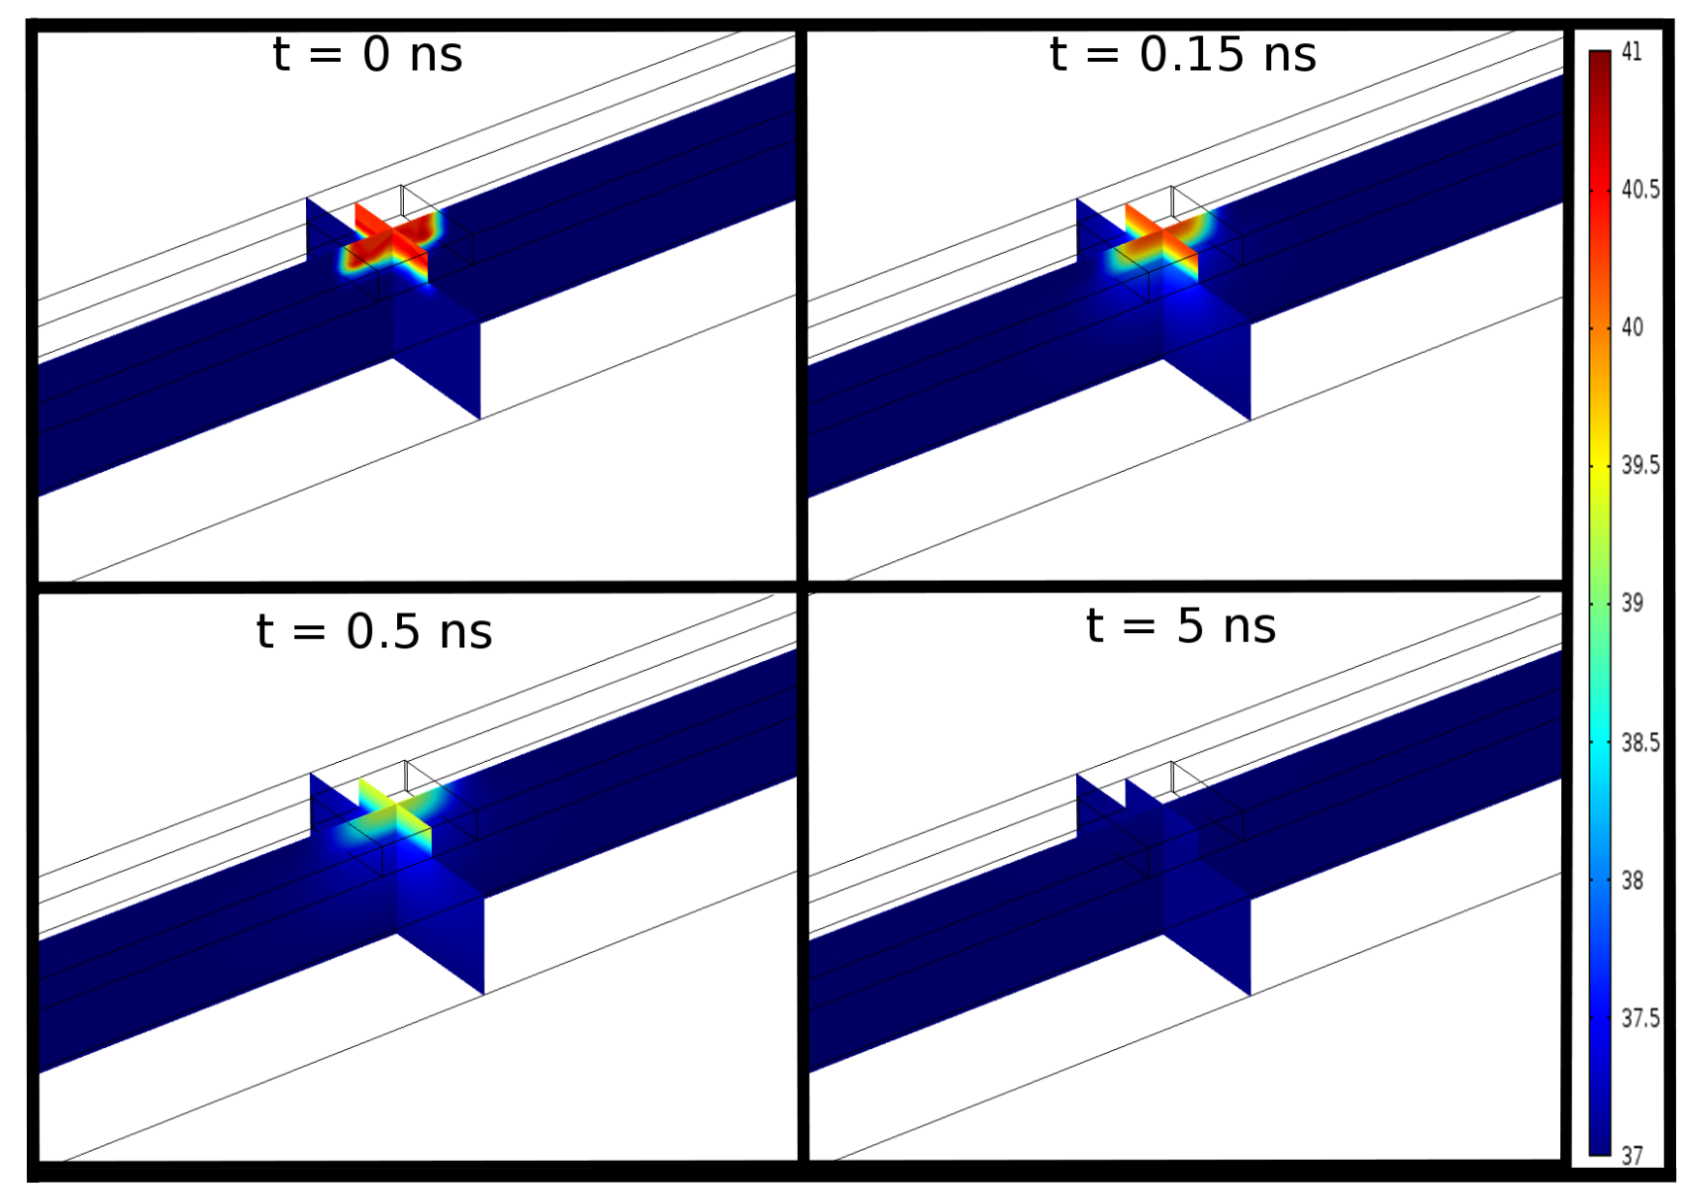
\includegraphics[width=0.95\columnwidth,angle=0]{relax}
  \end{center}
  \caption[Temperatura del detector para diferentes tiempos.]{Temperatura del detector para diferentes tiempos. Se muestra un alambre de MgB$_2$ de 15\,x\,2\,x\,0.8\,$\mu$m depositado sobre un sustrato de Si de 15\,x\,4\,x\,2\,$\mu$m.}
\label{fig:cortes}
\end{figure}

Se aprecia que la región más caliente del detector es siempre la misma, es decir, parece ser que el calor tiende a difundir mucho más a través del sustrato que dentro del MgB$_2$. Teniendo en cuenta que la conductividad térmica del silicio es $\kappa_{\text{Si}}\,=\,3510$\,W/(m\,K) y la del MgB$_2$ es $\kappa_{\text{MgB}_2}\,=\,14.35$\,W/(m\,K)\cite{Glassbrenner1964,Bauer2001}, parece razonable que sea así. Resultados similares se obtuvieron al reemplazar el sustrato del Si con zafiro, lo cual también tiene sentido ya que $\kappa_{\text{zafiro}}\,=\,12000$\,W/(m\,K)\cite{Ekin2006}.
\nomenclature{$d$}{Espesor de un film o cable.}
\nomenclature{$l$}{Longitud de un cable.}
\nomenclature{$a$}{Ancho de un cable.}
\nomenclature{$\kappa$}{Conductividad térmica.}
\nomenclature{$c_p$}{Calor específico a presión constante.}
\nomenclature{$A$}{Área del detector.}
\nomenclature{$V_{hs}$}{Volumen en que se deposita la energía de una reacción.}
\nomenclature{$\delta$}{Densidad de un material.}
\nomenclature{$\rho$}{Resistividad de un material.}
\nomenclature{$T_{hs}$}{Temperatura que alcanza el volumen en donde se deposita la energía de la reacción.}
\nomenclature{$T_o$}{Temperatura de operación del detector.}
\section{Señal del detector}\label{S:signal}
Como se dijo antes, el atributo característico de los detectores TES es que obtienen una muy buena señal al aprovechar los cambios abruptos de la resistividad de un film superconductor. El propósito de esta sección es estimar la señal producida por un detector de MgB$_2$ al capturar un neutrón y calcular la temperatura óptima de operación del dispositivo, definida como aquella en que la variación de la resistencia producida por la captura de un neutrón sea máxima. En lo que sigue, los términos señal y variación de la resistencia se utilizarán como sinónimos, ya que la señal emitida por el detector es proporcional a la variación de la resistencia del MgB$_2$.

Se estudió la variación de la resistencia $\Delta R$ en el volumen $V_{hs}$ en función de la temperatura inicial del mismo. Para este estudio se consideró un modelo diferente al de la sección anterior, es decir, se consideró que el volumen $V_{hs}$ tiene ancho y espesor iguales a los del cable de MgB$_2$, pero para este modelo se consideró una longitud fija. El cambio en la resistencia del alambre $\Delta R$ se calculó a partir de la relación\cite{Sears1964}:
\begin{equation}
  \Delta R \ = \ \frac{\Delta \rho \ l}{a \ d}
  \label{eq:DR}
\end{equation}
\noindent
siendo $l$, $a$ y $d$ la longitud, el ancho y el espesor del volumen $V_{hs}$, respectivamente. Se tomaron valores de $a \, = \, 2\,\mu$m, $0.2\, \mu m \, \leq \, d \, \leq \, 1\,\mu$m y $l \, = \, 2\,\mu$m. La variación de $\rho$ en función de la temperatura se obtuvo a partir las mediciones obtenidas de \cite{Nagamatsu2001} y que se ven en la Fig.\,\ref{fig:rovsT}.
\begin{figure}[tbh!]
 \begin{center}
    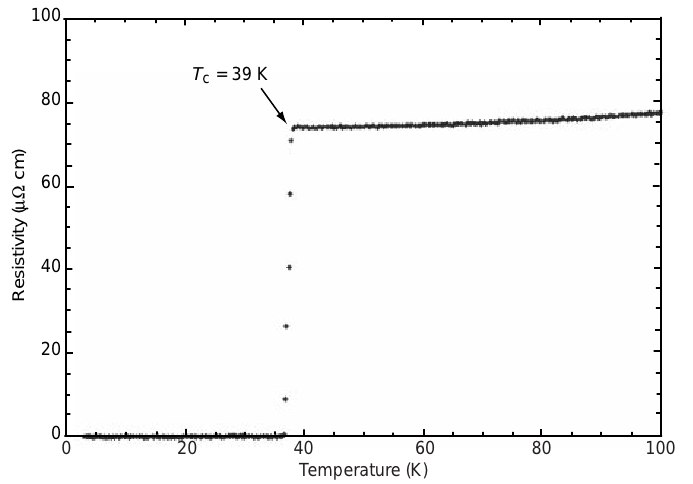
\includegraphics[width=0.75\textwidth]{rovsT}
  \end{center}
  \caption[Variación de la resistividad del MgB$_2$ en función de la temperatura.]{Variación de la resistividad del MgB$_2$ en función de la temperatura. Puede verse el cambio abrupto en la resistividad del MgB$_2$ a 39 K. Imagen obtenida de \cite{Nagamatsu2001}.}
\label{fig:rovsT}
\end{figure}

En la Fig. \ref{fig:rvsT} se muestra como varía la señal del alambre de MgB$_{2}$ en función de la temperatura inicial, comparando el resultado para diferentes espesores. Puede observarse que el cambio en la señal es del orden de algunos Ohm y que la misma decrece fuertemente a medida que el cable se vuelve más grueso. También puede apreciarse que incrementar el espesor del cable obliga a tener un control más estricto de la temperatura. Dicha conclusión es razonable dentro del modelo propuesto, ya que un espesor menor implica que la misma energía de la reacción se deposita en una región de material que es más pequeña. Esto trae aparejado que el incremento de temperatura sea mayor, lo que simplifica el control de la misma.
\begin{figure}[tbh!]
 \begin{center}
    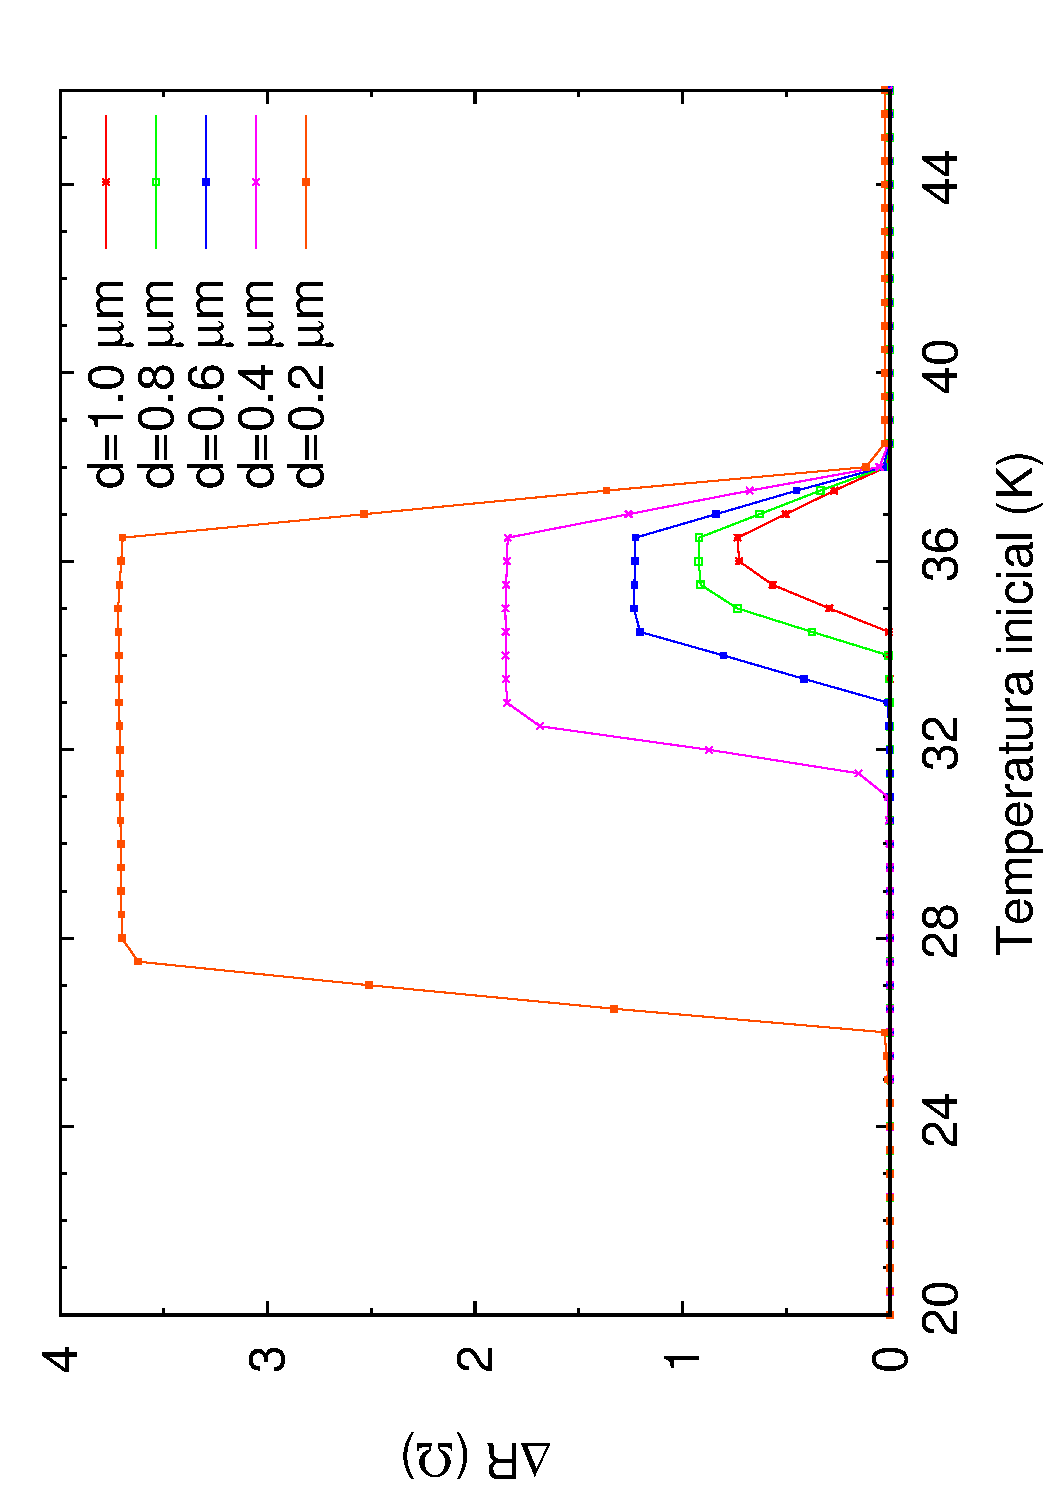
\includegraphics[width=0.5\textwidth, angle=-90]{rvst}
  \end{center}
  \caption[Variación de $\Delta$R en función de la temperatura inicial del MgB$_2$.]{Variación de $\Delta$R en función de la temperatura inicial del MgB$_2$. Las dimensiones de la porción de MgB$_2$ eran  2\,$\mu$m\,x\,2\,$\mu$m\,x\,$d$\,nm.}
\label{fig:rvsT}
\end{figure}
%\newpage

Sin embargo, es válido preguntarse si es correcto pensar que la energía que se deposita en el cable es independiente de las dimensiones del mismo, ya que si el cable se vuelve más delgado los iones escaparían del mismo antes de depositar toda su energía en el MgB$_2$. Siguiendo esta motivación se realizaron simulaciones estudiando el cambio en la señal disminuyendo la energía que se deposita en el detector. El volumen $V_{hs}$ se modeló de la misma forma que en el cálculo anterior, considerando solamente alambres de 200\,nm y 800\,nm de espesor, como se puede ver en la Fig. \ref{fig:RvsrvsQ}. 

\begin{figure}[h!]
 %\centering
  \hspace{-1.4cm}
 \subfloat[200\,nm]{\label{fig:R1}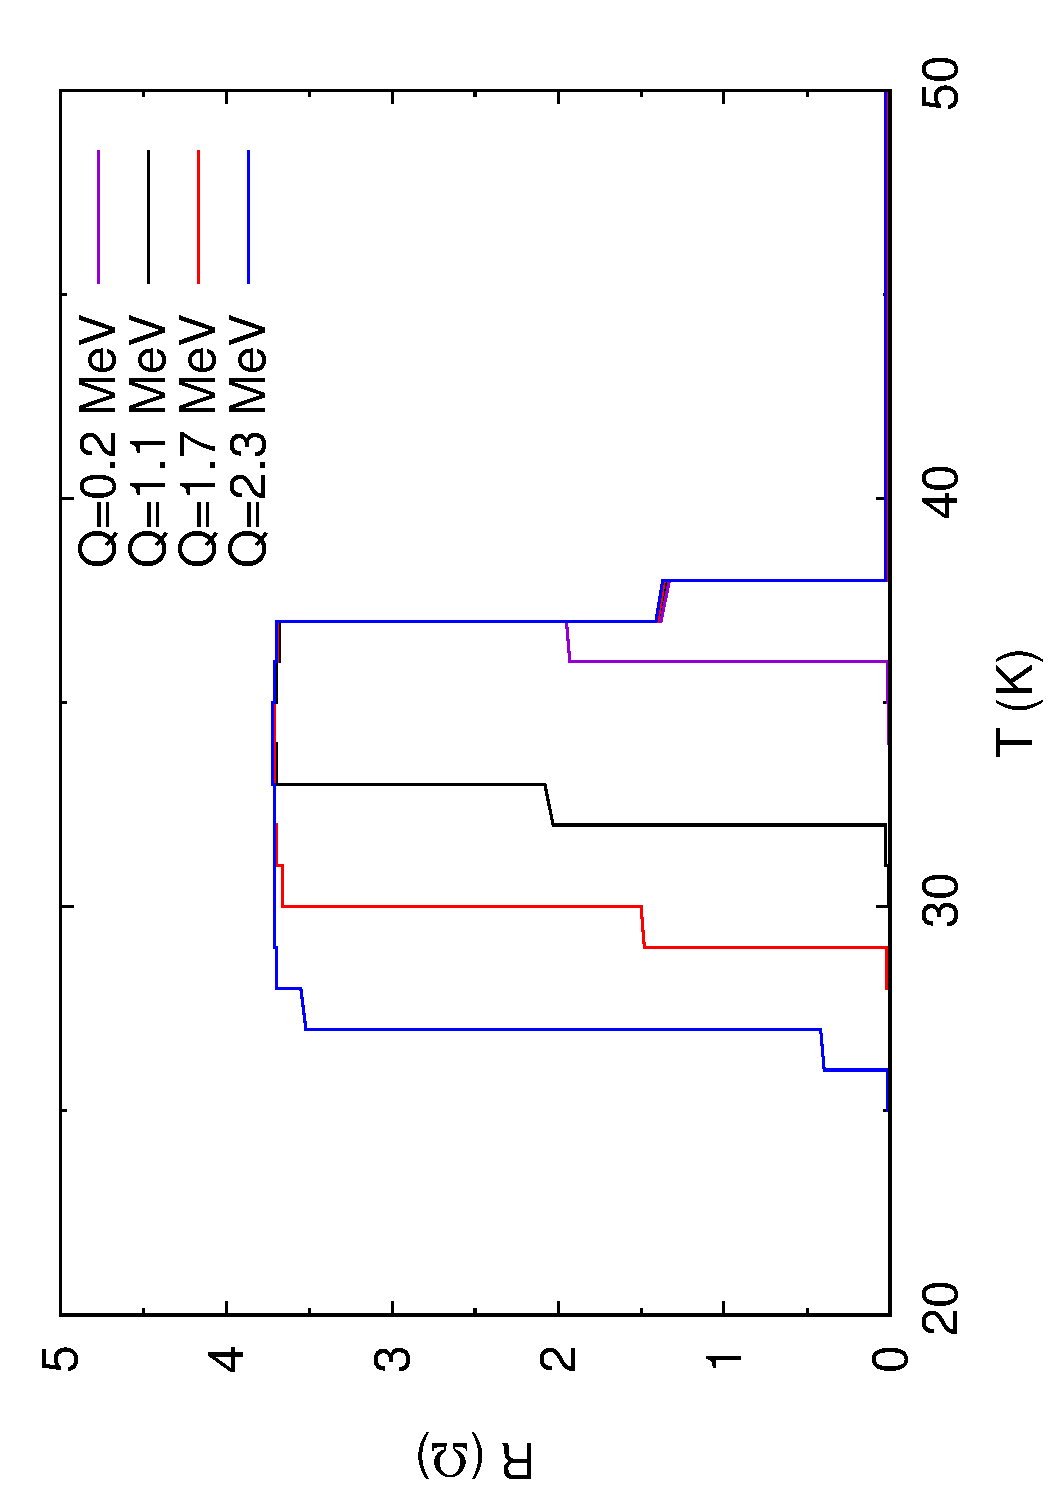
\includegraphics[width=0.4\columnwidth,angle=-90]{RvsTvsQ_200nm}}
 \subfloat[800\,nm]{\label{fig:R2}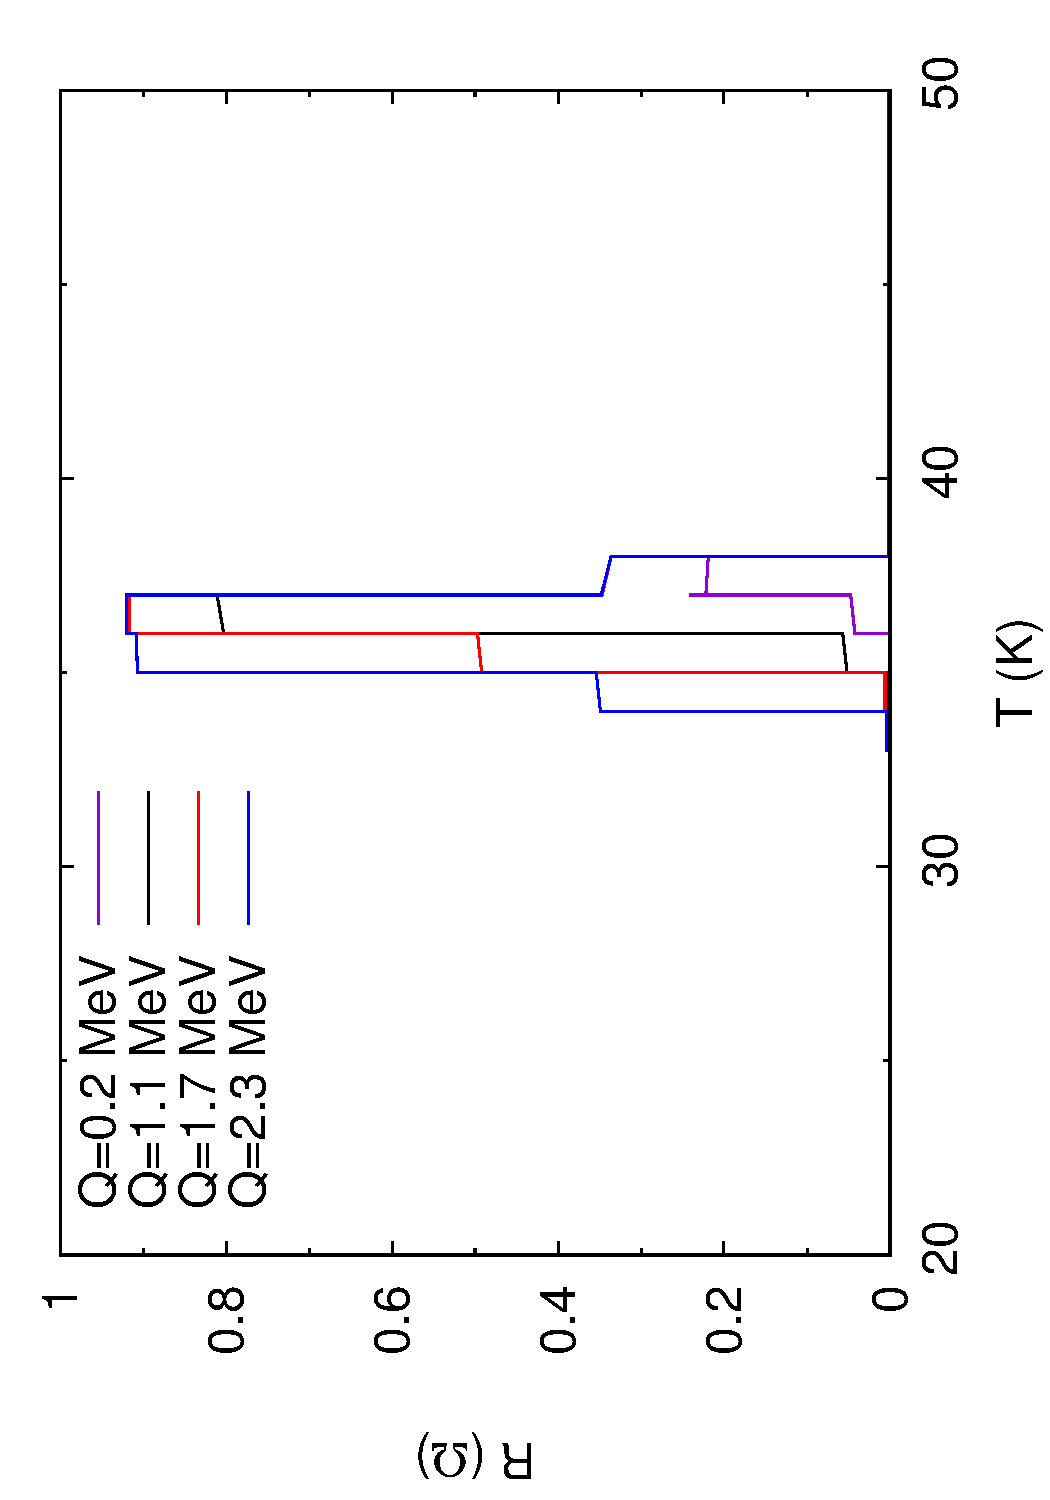
\includegraphics[width=0.4\columnwidth,angle=-90]{RvsTvsQ_800nm}}
   \caption[Señal producida por el detector en función de la temperatura de operación y la energía depositada en el mismo.]{Señal producida por el detector en función de la temperatura de operación y la energía depositada en el mismo. En la Fig. \ref{fig:R1} se muestra el cálculo realizado para un cable de un espesor de 200\,nm mientras que en la \ref{fig:R2} aparece el resultado para un cable de 800\,nm. A partir de comparar estos gráficos es claro ver que un cable delgado produce una mayor señal que uno más grueso, incluso si en el cable delgado se deposita una energía diez veces menor que en el grueso.}
\label{fig:RvsrvsQ}
\end{figure}

%\newpage
Con los datos de la Fig. \ref{fig:RvsrvsQ} junto con los análisis hechos previamente se puede hacer un estudio más integral de las ventajas y desventajas de las diferentes geometrías del detector. Por ejemplo, en la Fig. \ref{fig:R1} puede verse que si el espesor del cable de MgB$_{2}$ es de 200\,nm se tiene una señal que es mayor que la que se puede esperar para un alambre de 800\,nm, incluso si en el cable se deposita una energía diez veces menor. En ese sentido, la misma conclusión puede extraerse si la variable a analizar es la temperatura óptima de operación del detector, ya que de comparar las Figs. \ref{fig:R1} y \ref{fig:R2}, puede verse que el intervalo en que se observa un máximo de señal para un film de espesor de 200\,nm, es siempre igual o mayor al intervalo esperado para un film de 800\,nm, sea cual sea la energía que se deposita en el detector.
\section{Acoplamiento térmico-eléctrico}\label{S:termyelec}
En las secciones anteriores se estudió por un lado como se enfría una sección de MgB$_2$ sobre un sustrato que se mantiene a una temperatura fija. Por otro lado se mo\-de\-ló y calculó también la modificación de la resistencia de un cable de MgB$_2$ como resultado de la captura de un neutrón. Si se observa con un poco de cuidado, puede verse que en un cable de MgB$_2$ diseñado adecuadamente aparecen dos fenómenos interesantes. El primero es el ''efecto fusible'', es decir que la diferencia de tensión en los extremos de un cable se incrementa súbitamente debido a la reacción que se inicia con la absorción de un neutrón. El segundo es que debido a que una porción importante del material deja de ser superconductor, el mismo se convierte en una fuente de calor, debido al efecto Joule. Este acoplamiento que ocurre entre el sistema térmico y el eléctrico, puede considerarse despreciable si las corrientes circulantes son lo suficientemente bajas. Sin embargo, debido al comportamiento altamente no lineal que tiene la resistividad del MgB$_2$ alrededor de la transición superconductora, es razonable preguntarse qué tan baja debe ser la corriente circulante para ser considerada despreciable. De aquí se concluye que hacer un estudio acoplando el problema térmico y el eléctrico resulta necesario si se quieren determinar las condiciones de operación óptimas del detector. Además, la inclusión de una fuente de calor en el problema podría modificar el tiempo de respuesta del detector, detalle que puede ser importante si se busca un equipo que trabaje con elevados flujos de neutrones.

En este punto parece apropiado comentar algunas de las complicaciones que aparecen cuando se busca resolver un problema que se representa por un sistema de ecuaciones diferenciales acopladas (la ecuación de transferencia del calor y la de los circuitos de corriente continua). Este acoplamiento puede resultar complicado, sobre todo si el mismo se hace a través de una variable que tiene un comportamiento no lineal, como lo es la resistencia del MgB$_2$ en este caso. Los mayores problemas que aparecen son la aparición de inestabilidades, oscilaciones, soluciones espurias y que el programa falle en poder satisfacer las condiciones de borde exigidas. Luego de algún trabajo y estudio del programa utilizado para hacer las simulaciones, se encontró que la mejor forma de solucionar estos problemas es la siguiente: primero se resuelve el problema eléctrico para la condición inicial (tal como fue planteada en la sección \ref{S:term}) sin tener en cuenta la evolución temporal del sistema. Una vez logrado esto se toman los datos (corrientes y tensiones) de esta simulación y se los utiliza como condición inicial del problema térmico-eléctrico dependiente del tiempo.

En adición a las simulaciones que permitieron estimar el tiempo de respuesta, se llevó a cabo una simulación más para estimar las dimensiones mínimas que debe tener el detector para que pueda detectar neutrones eficientemente. En este caso se consideró un bloque de MgB$_2$ que se encuentra en estado superconductor. Se supuso que la captura de un neutrón causó una supresión del parámetro de orden superconductor en un cubo de 0.2\,$\mu$m de lado\cite{Machida2004}. Por lo tanto se consideró que la energía de la reacción se depositó inicialmente en ese volumen. Se puso al bloque de MgB$_2$ en contacto directo con una fuente térmica fría, y se lo conectó a una fuente eléctrica de corriente continua. El objetivo de esta simulación era ver el tamaño máximo que adquiría la región normal, es decir, no superconductora, del MgB$_2$.
\begin{figure}[h!]
 \begin{center}
    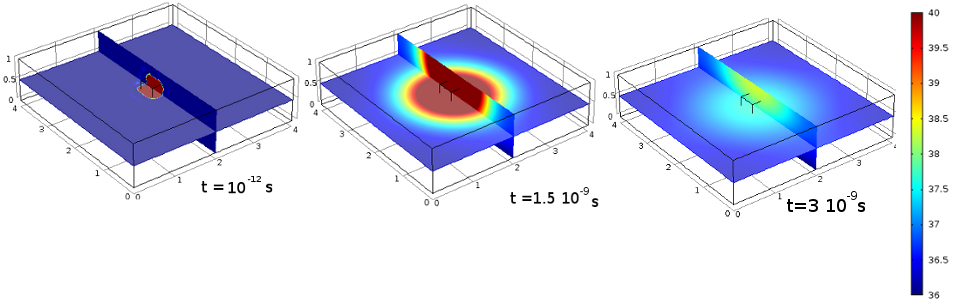
\includegraphics[width=\columnwidth]{secuencia3}
  \end{center}
  \caption[Secuencia temporal que indica como fluye el calor desde el ''punto caliente'' inicial hacia el resto del material.]{Secuencia temporal que indica como fluye el calor desde el ''punto caliente'' inicial hacia el resto del material. Se muestran dos cortes transversales del bloque de MgB$_2$ simulado. La parte inferior del bloque se mantuvo a 36\,K. El espesor del bloque era de 1\,$\mu$m. Puede verse como la región del material que se vuelve normal tiene un tamaño máximo del orden de 1\,$\mu$m antes de empezar a hacerse más pequeña.}
\label{fig:secuencia}
\end{figure}

Así como se hizo en la sección \ref{S:term}, el estudio del acoplamiento de los problemas térmico y eléctrico también se hizo utilizando el software comercial COMSOL MULTIPHYSICS. Se consideró como ecuación constitutiva $\mathbf{J} \, = \, \sigma(T) \, \mathbf{E}$ y se incorporó la disipación debida al efecto Joule ($\dot{q} \, = \, J^2/\sigma$). La conductividad eléctrica $\sigma(T)$ se obtuvo de la curva de resistividad de una muestra bulk de MgB$_2$ que se muestra en la Fig \ref{fig:rovsT}, al igual que en la sección \ref{S:signal}. En la Fig. \ref{fig:secuencia} se pueden apreciar dos cortes perpendiculares que muestran el campo de temperaturas en el bloque de MgB$_{2}$ en distintos momentos de la simulación: el instante inicial, el instante en el que la región normal ocupó el máximo volumen y un instante posterior en que el sistema estaba prácticamente en equilibrio térmico. A partir de estas imágenes se puede observar que la región normal adquiere una forma esférica cuyo radio máximo es un poco mayor que un micrón y que luego empieza a hacerse más pequeño. Esto implica que un cable de MgB$_2$ cuyo ancho y espesor sean mucho mayores que un micrón no detectará eficientemente la captura de un neutrón, ya que es altamente probable que incluso en el momento en que la región normal tome su tamaño máximo, aún exista un paralelo superconductor por el que circulará la mayoría de la corriente aplicada. Un análisis similar al previo se hizo reduciendo el espesor del bloque de MgB$_2$ a 0.5\,$\mu$m y 0.2\,$\mu$m. Se pudo apreciar que si bien el tiempo de relajación del sistema disminuye, el tamaño máximo de la región normal aún es del orden de un micrón. La conclusión que se puede hacer entonces concuerda con la extraída de las secciones \ref{S:term} y \ref{S:signal}, y es que para poder tener una buena sensibilidad ante la captura de un neutrón, es necesario que tanto el espesor del cable como su ancho sean de dimensiones del orden o inferiores al micrón.
\nomenclature{$\sigma$}{Conductividad eléctrica.}

También se estudió el comportamiento de las simulaciones de la sección \ref{S:term} agregando la componente eléctrica del problema. Las condiciones de contorno para la parte térmica de la simulación eran las mismas que las que se utilizaron para la sección \ref{S:term}. Se trabajó en el problema eléctrico suponiendo que el detector operaba tanto a corriente constante como a tensión constante.
\subsection{Simulaciones a corriente constante}\label{ss:Icte}
Se hicieron simulaciones a diferentes corrientes en el rango de 1\,$\mu A$ y 100\,$m A$ para espesores de 200\,$nm$ y 1000\,$nm$, y se estudió la diferencia de potencial entre los extremos del alambre, así como la variación de la temperatura del mismo en función del tiempo.

A partir de las simulaciones se encontró que existe una corriente a partir de la cual la temperatura del sistema no tiende asintóticamente a la inicial, lo cual es lógico, ya que si la disipación Joule produce suficiente calor como para mantener la temperatura del cable por encima de $T_c$, el sistema nunca vuelve al estado superconductor, ya que el MgB$_2$ nunca se enfría lo suficiente como para que la resistividad empiece a disminuir. El valor de esta corriente umbral depende de la forma del alambre de MgB$_2$ pero para las geometrías simuladas se encontró que tiene un valor que está entre la decena y la centena de miliamperes. 
\begin{figure}[h!]
 \begin{center}
    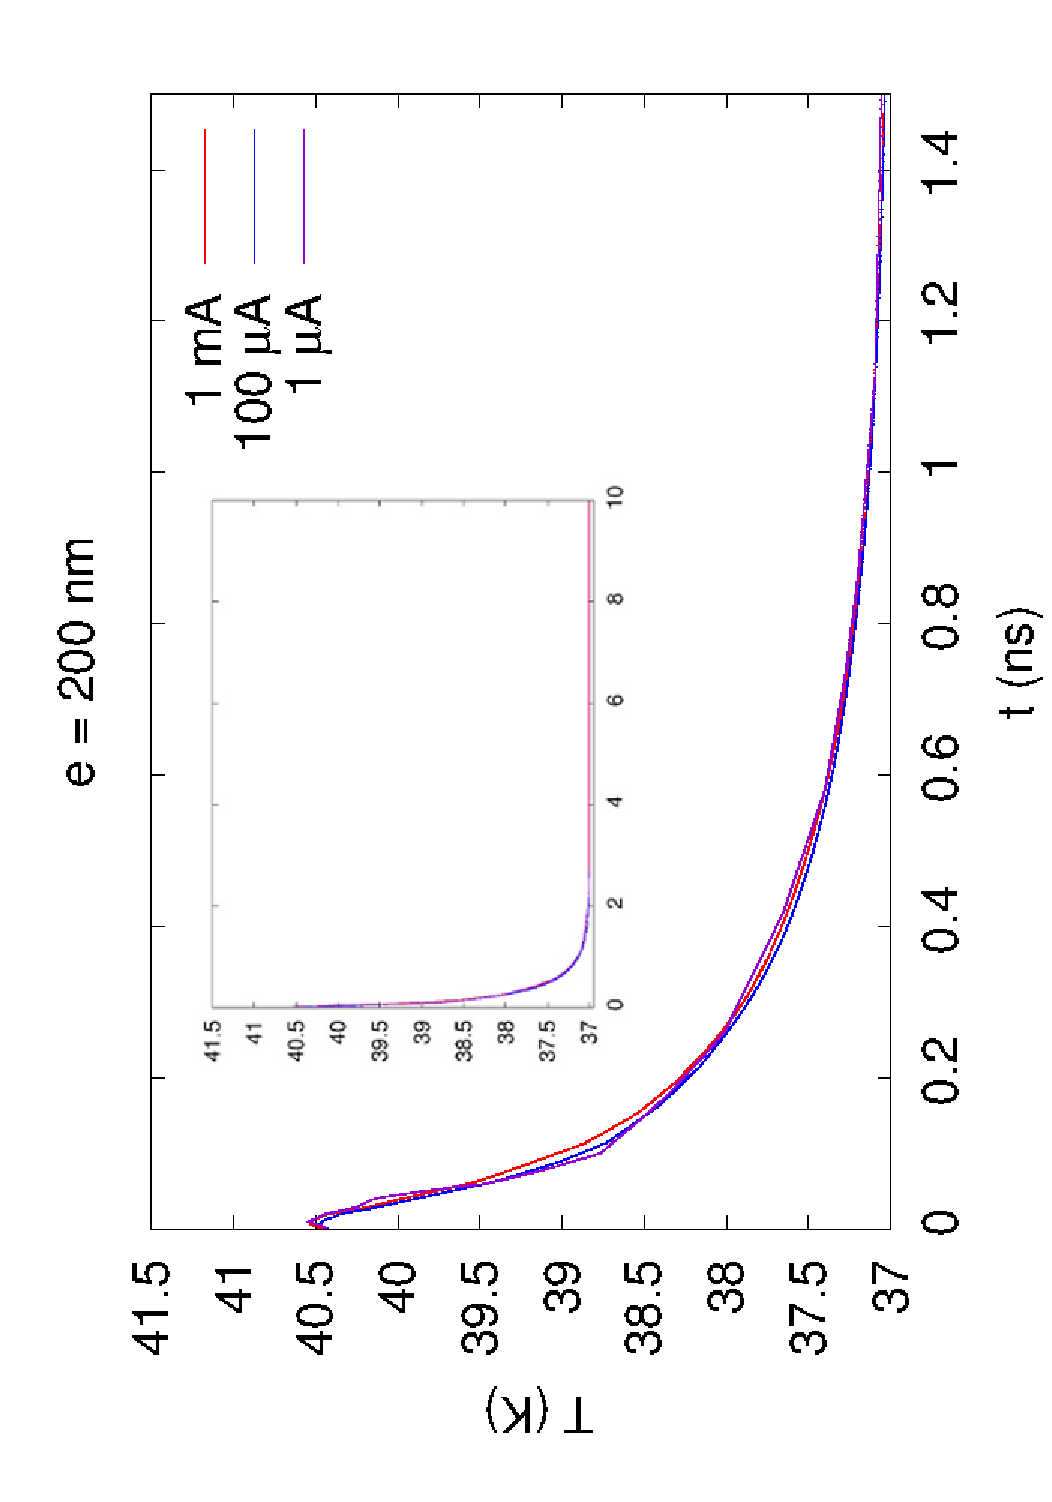
\includegraphics[width=0.5\columnwidth, angle=-90]{TvstxI}
  \end{center}
  \caption[Temperatura en función del tiempo para un alambre de MgB$_2$ de 200\,$nm$ espesor y con diferentes corrientes circulantes.]{Temperatura en función del tiempo para un alambre de MgB$_2$ de 200\,$nm$ espesor y con diferentes corrientes circulantes. Se observa que el tiempo de relajación es prácticamente independiente de la corriente circulante.}
\label{fig:TvstxI}
\end{figure}

Por otro lado, si la corriente que circula por el MgB$_2$ está por debajo de este umbral, el tiempo de relajación del sistema parece ser independiente de la misma, como se puede ver en la Fig. \ref{fig:TvstxI}. Además, en la Fig. \ref{fig:TvstxexI} se aprecia que no existe una diferencia significativa en el tiempo de relajación cuando se desacopla el problema eléctrico del térmico. De aquí puede concluirse que en el régimen estable el calentamiento debido al efecto Joule no juega un rol significativo en la dinámica del sistema.

\begin{figure}[h!]
 \begin{center}
    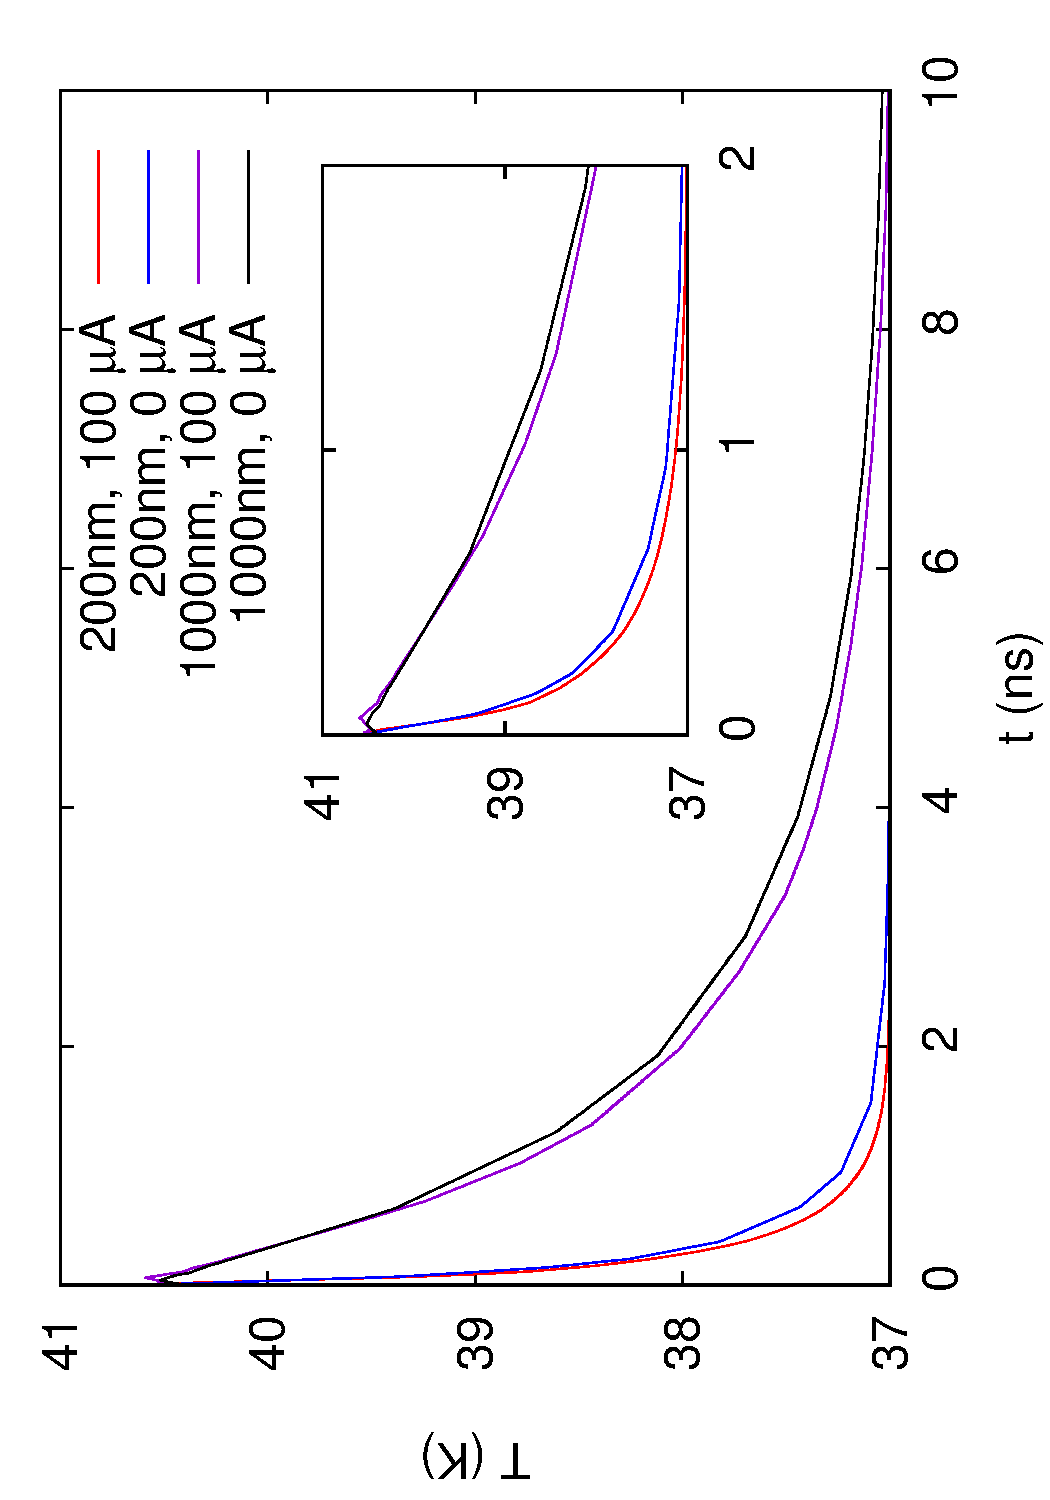
\includegraphics[width=0.5\columnwidth, angle=-90]{TvstxexI}
  \end{center}
  \caption[Comparación del tiempo de relajación para un alambre de MgB$_2$ para el caso desacoplado y acoplado.]{Comparación del tiempo de relajación para un alambre de MgB$_2$ para el caso desacoplado (corriente 0) y acoplado. No se observan diferencias apreciables entre los dos casos.}
\label{fig:TvstxexI}
\end{figure}

Por último se estudió cómo varía la señal del detector en función del tiempo, para lo cual se graficó la evolución temporal de la resistencia del alambre de MgB$_2$. En la figura \ref{fig:signal} se compara además cómo varía la respuesta para cables de diferentes espesores. Puede verse como al aumentar el espesor del alambre el pico de la señal se vuelve más ancho y de menor altura. 
\begin{figure}[h!]
 \begin{center}
    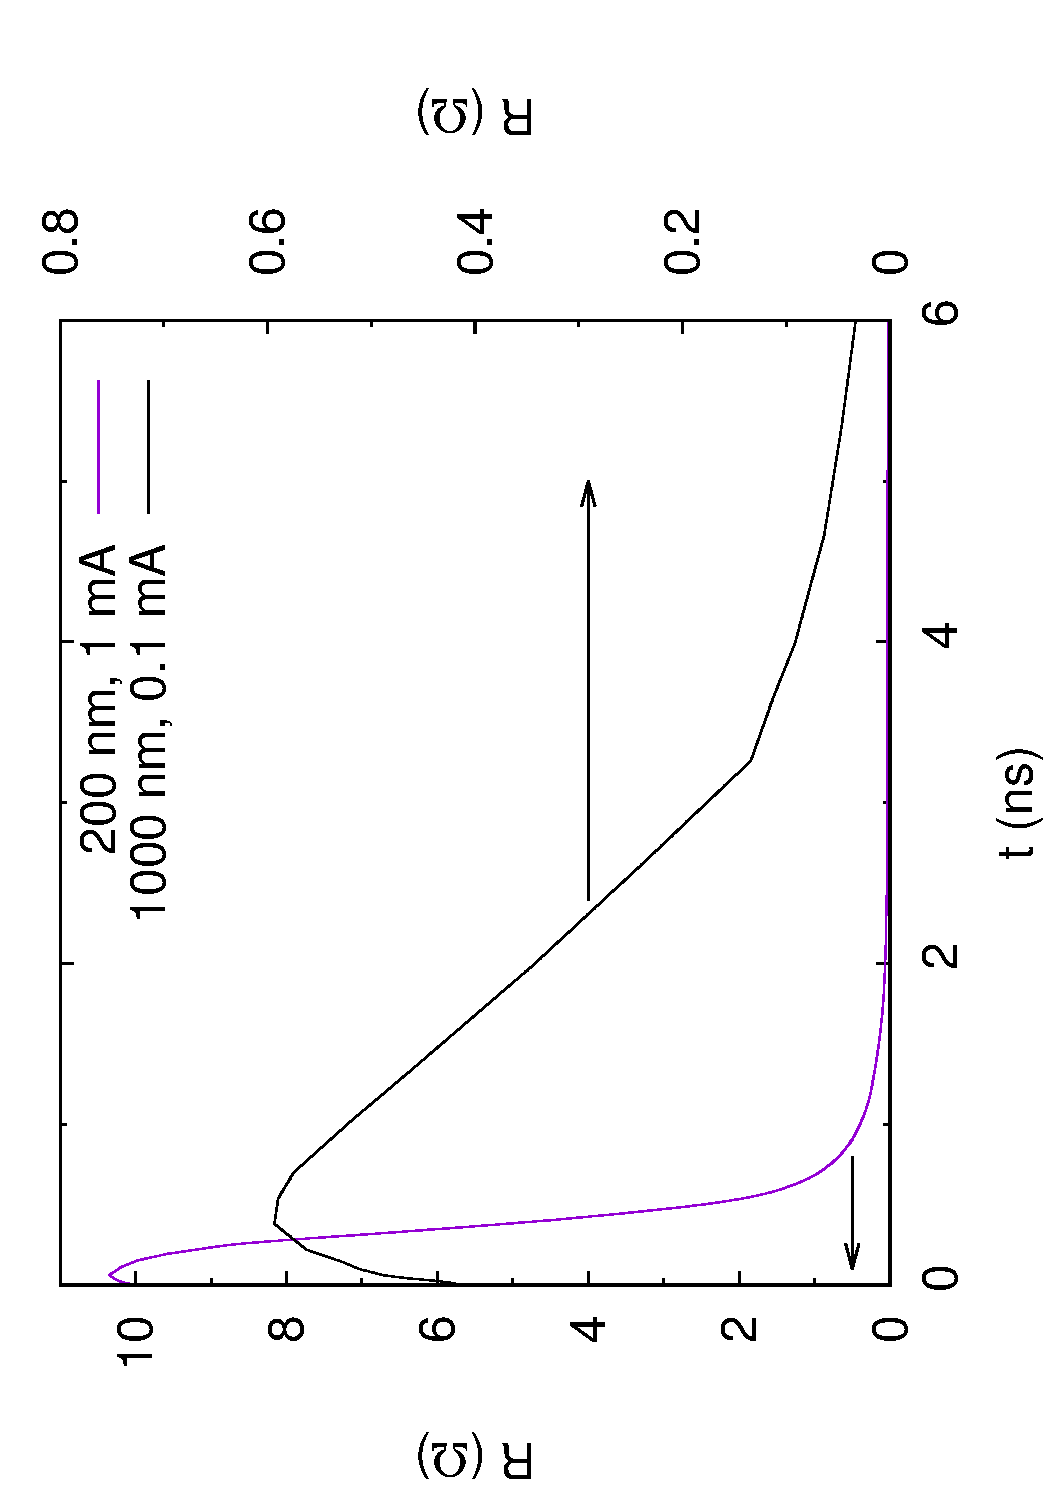
\includegraphics[scale=0.55, angle=-90]{signal}
  \end{center}
  \caption[Resistencia en función del tiempo de dos alambres de MgB$_2$, uno de 1000 nm de espesor y otro de 200 nm de espesor.]{Resistencia en función del tiempo de dos alambres de MgB$_2$, uno de 1000 nm de espesor y otro de 200 nm de espesor. El resto de las dimensiones son equivalentes. Se observa que los pico de resistencia se vuelven más anchos y más bajos a medida que aumenta el espesor del alambre.}
\label{fig:signal}
\end{figure}

En la sección \ref{S:eficiencia} se mostrará la dependencia de la eficiencia del detector con el espesor del mismo.  Allí se muestra que la probabilidad de captura de un neutrón es proporcional al espesor del detector. Esto es, si el espesor del detector se incrementa en un factor 5, también lo hace la probabilidad de captura. En la Fig. \ref{fig:signal} puede verse que un incremento en un factor 5 de la eficiencia redunda en un detrimento en un factor 10 en el valor de la señal. También implica un notable alargamiento en el tiempo de respuesta, lo que puede ser deseable en función de la electrónica de seguimiento que se disponga. Sin embargo, esto también se puede lograr a partir de crecer el detector en una estructura tipo membrana, de lo que se concluye finalmente que no es recomendable buscar un mayor espesor del detector, puesto que la ganancia en eficiencia no parece compensar los aspectos negativos asociados a un detector de mayor volumen.
\subsection{Simulaciones a tensión constante}\label{ss:Vcte}
En la sección \ref{S:tes} se explicó que si un TES se  opera a tensión constante, se puede utilizar el efecto Joule como mecanismo de control de la temperatura de operación del detector. Para lograr esto, es necesario que la temperatura de la fuente fría se encuentre muy por debajo de la $T_c$ del material que se usa como volumen de detección. Cabe mencionar que los dispositivos en los que este mecanismo se implementa con éxito son aquellos materiales que tienen una transición superconductora a temperaturas del orden de los cientos de milikelvin. El propósito de esta sección es estudiar la viabilidad de implementar un control de temperatura utilizando únicamente el efecto Joule como señal de realimentación. El poder lograr esto sería extremadamente conveniente, ya que en ese caso se evita la necesidad de incorporar equipos extra para realizar un control de la temperatura, simplificando así la construcción del dispositivo.
 \begin{figure}[tbh!]
   \begin{center}
	 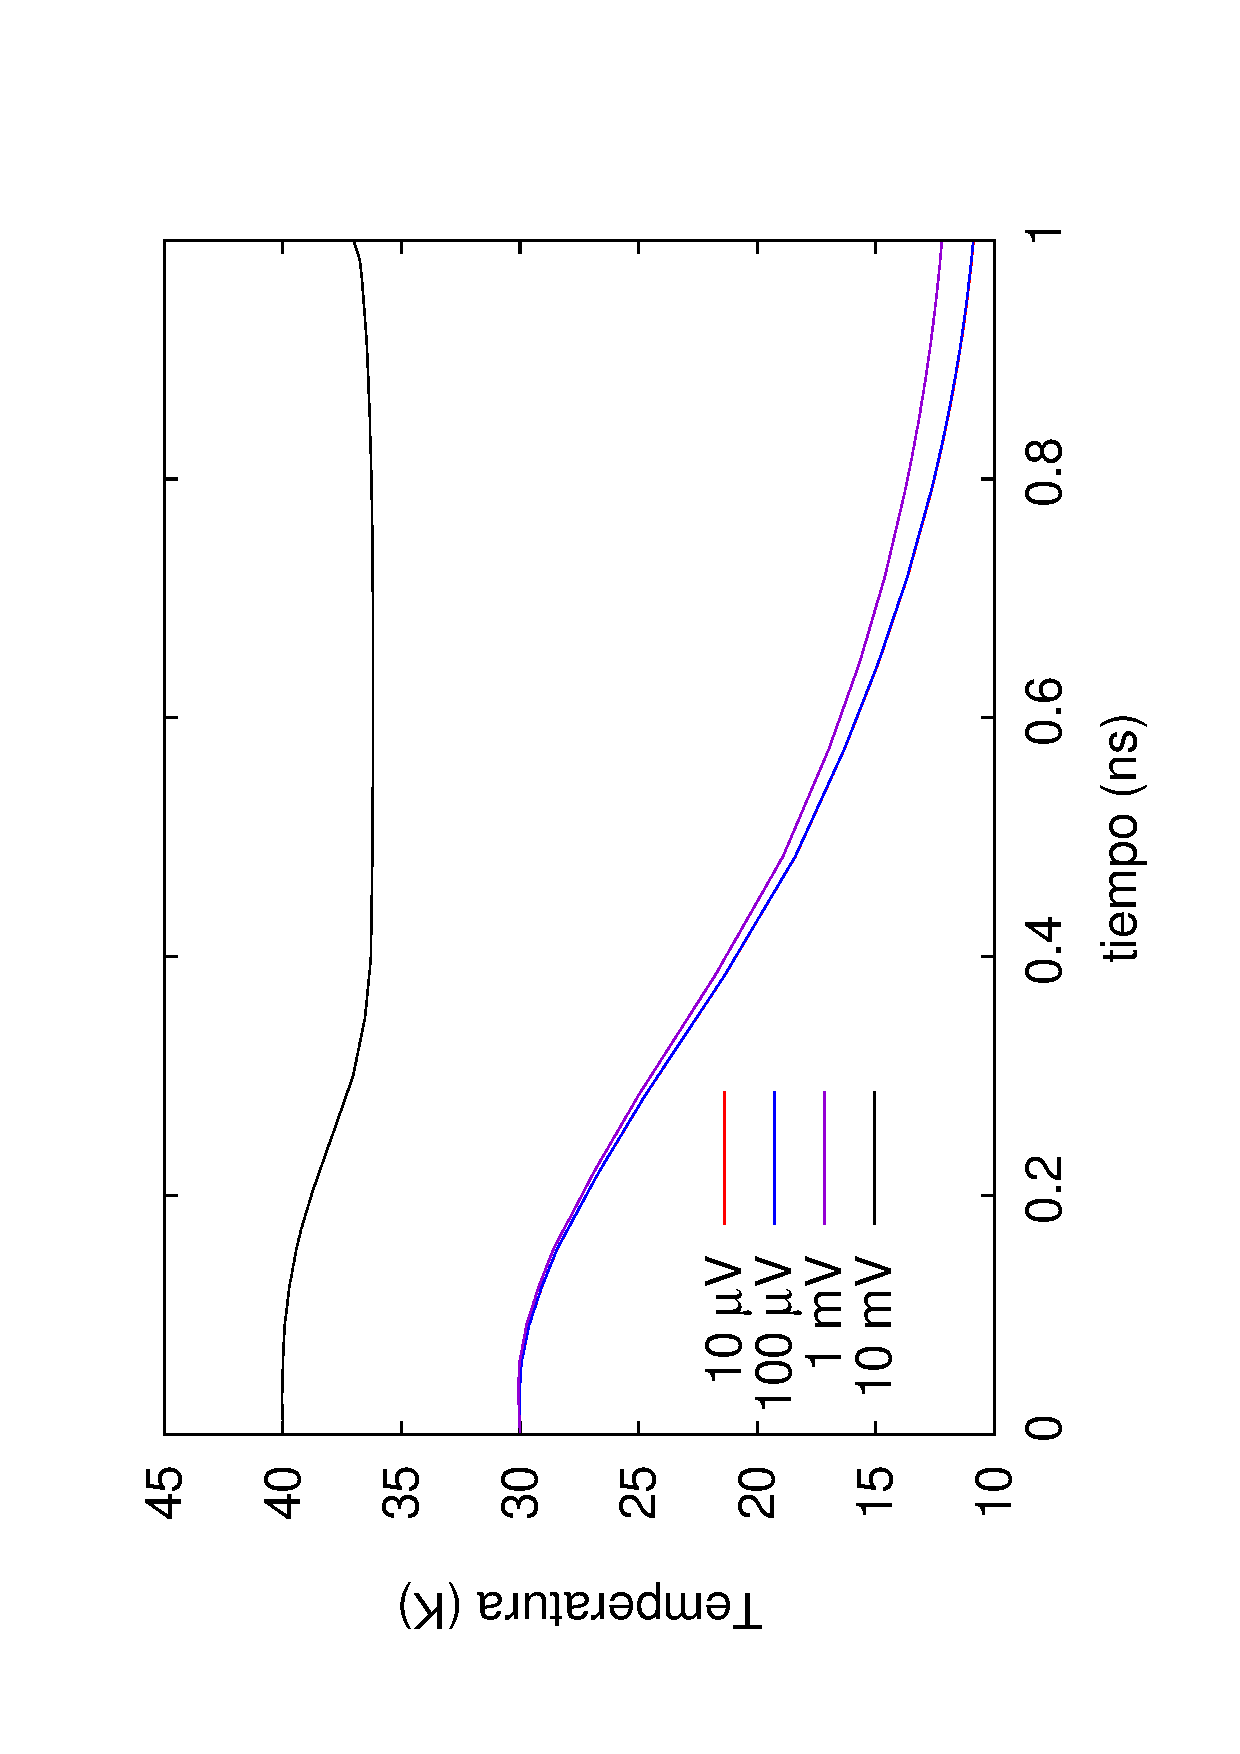
\includegraphics[width=0.95\columnwidth]{Tvst_Vest_200x1}
   \end{center}
   \caption[Estudio de la variación de la temperatura en función del tiempo para un detector operado a tensión constante, variando la tensión de operación.]{Estudio de la variación de la temperatura en función del tiempo para un detector operado a tensión constante, variando la tensión de operación. La fuente fría se mantuvo a 10\,K. Puede verse que que al incrementar la tensión la temperatura a la que estabiliza el sistema se incrementa tambi\'en.}
   \label{fig:TvstxV}
 \end{figure}

Para realizar este estudio se simuló un cable con una geometría similar a la de las secciones anteriores, analizando sólo el caso de un detector de 200\,nm de espesor. Se dispuso que la temperatura de la fuente fría fuera de 10\,K. Se eligió esta temperatura considerando que es la mínima alcanzable por un criogenerador comercial Gifford-MacMahon, que es un equipo criogénico con un costo accesible. Se propuso como condición inicial que el cable de MgB$_2$ se encontrara a una temperatura de 30 o 40\,K para luego ver cómo variaba la temperatura del mismo con el tiempo. Se realizaron simulaciones para diferentes tensiones aplicadas en bornes del cable, y en la Fig. \ref{fig:TvstxV} puede verse como, mientras la tensión aplicada es baja, el sistema siempre relaja a la temperatura de la fuente fría. Por otro lado, a una tensión del orden de 10\,mV puede verse que la producción de calor debida al efecto Joule compensa la pérdida de energía hacia la fuente fría, y el sistema logra estabilizarse a una temperatura de trabajo razonable.
%\newpage
Sin embargo, el problema que aparece ahora es que la tensión que hay que aplicar obliga al paso de corrientes enormes por el detector, como puede verse en la Fig. \ref{fig:IvstxV}. Esto indica que, aunque es en principio posible controlar la temperatura de operación simplemente variando la tensión aplicada al detector, esto implica que a través del detector circularán corrientes que son inaceptables desde el punto de vista práctico.
  \begin{figure}[tbh!]
	\begin{center}
	  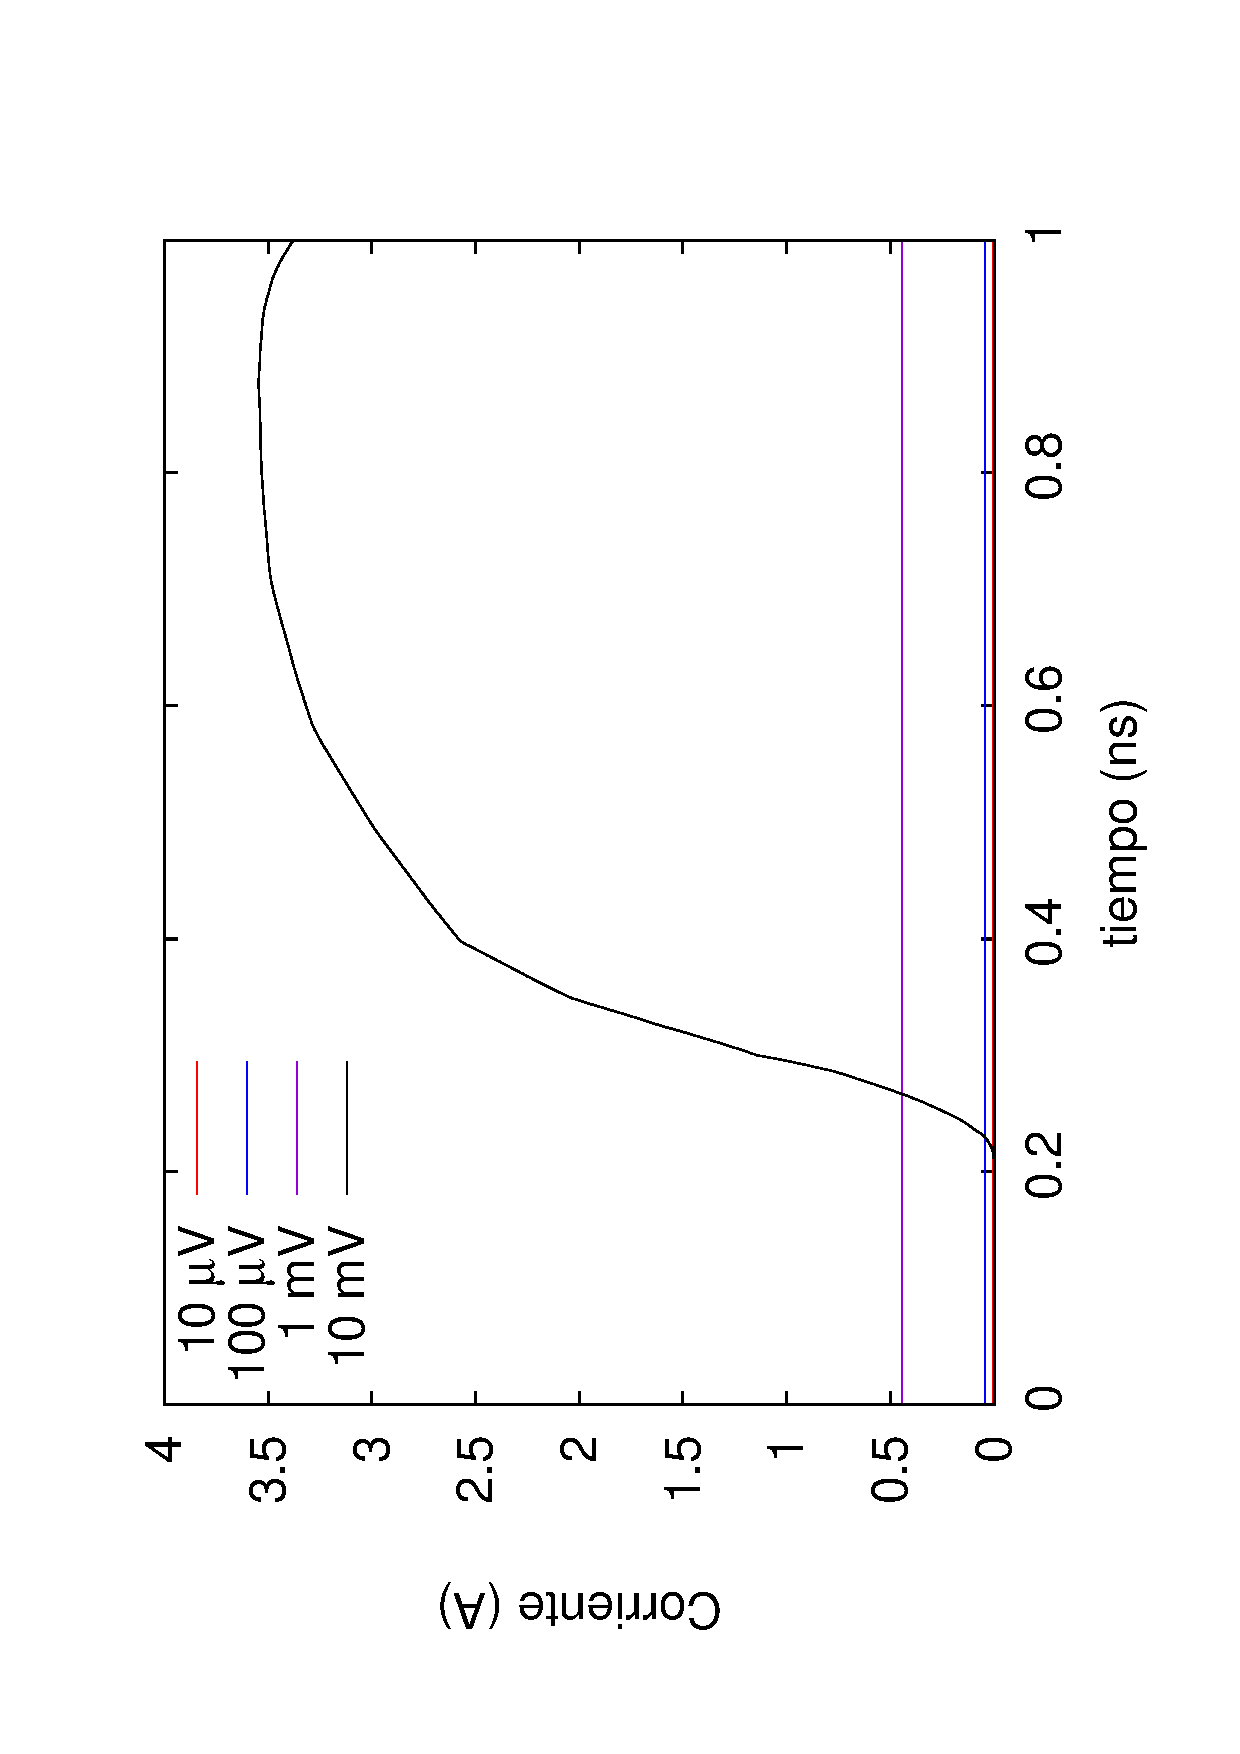
\includegraphics[width=0.55\columnwidth, angle=-90]{Ivst_200x1_Vest}
	\end{center}
	\caption[Cálculo de la corriente que circula por el detector en función de la tensión aplicada en función del tiempo.]{Cálculo de la corriente que circula por el detector en función de la tensión aplicada en función del tiempo. Como puede verse, el rango de tensiones útiles para controlar la temperatura del detector, implica el paso de grandes corrientes por el mismo. De aquí se concluyó que no es viable controlar la temperatura de operación del detector a partir de la tensión aplicada al mismo.}
	\label{fig:IvstxV}
  \end{figure}

Resulta por lo tanto, indispensable agregar un mecanismo externo para controlar la temperatura de operación del detector. Se pueden proponer dos mecanismos para lograr esto. Uno es simplemente controlar la temperatura de la fuente fría con un termómetro, un calefactor y un controlador de temperatura. También se puede pensar en depositar, entre el sustrato y el detector, algún material semiconductor que luego sea conectado a una fuente de corriente. De esta forma se implementa un mecanismo de control de temperatura utilizando la disipación Joule en el semiconductor como señal de realimentación, tal como se pretendía hacer con el propio detector.

Cabe mencionar, por último, que aunque controlar el detector con una fuente de tensión constante no sea un mecanismo viable para controlar la temperatura, sí resulta una opción atractiva por otras razones. Por un lado, al fijar la tensión y medir variaciones de corriente, se puede conseguir una buena amplificación de la señal simplemente poniendo en serie con el detector una inductancia\cite{Ishida2008}. Por otro lado tal como se explicó en la sección \ref{S:tes}, en caso de existir inhomogeneidades a lo largo del volumen del detector, si el mismo está regulado a corriente constante, el sistema se puede volver altamente inestable. Teniendo en cuenta estos detalles, es razonable concluir que el detector debe operarse a tensión constante.
\section{Eficiencia del detector}\label{S:eficiencia}
Para realizar el cálculo de la eficiencia del detector se partió de la ecuación de transmisión de neutrones para el caso de un sólo tipo de núcleo\cite{knoll}:
\begin{equation}
 \phi \ = \ \phi_0 \, e^{-n S d}
  \label{eq:t1}
\end{equation}
\noindent
siendo $\phi_0$ y $\phi$ el flujo inicial y final de neutrones, respectivamente, $n$ la densidad de núcleos por unidad de volumen, $S$ la sección eficaz total para la interacción núcleo-neutrón y $d$ el espesor de la muestra. La transmisión $\mathcal{T}$ se define como:
\begin{equation}
 \mathcal{T} \ = \ \frac{\phi}{\phi_0} \ = \ e^{-n S d}
  \label{eq:T}
\end{equation}
\noindent
Adicionalmente se puede definir el camino libre medio de un neutrón en el material considerado como la inversa del producto de la sección eficaz de interacción y la densidad la densidad de núcleos por unidad de volumen, es decir, si se nota como $\lambda_n$ al camino libre medio de un neutrón en el detector se puede escribir:
\begin{equation}
 \lambda_n \ = \ \frac{1}{n S}
  \label{eq:camino}
\end{equation}

Como $\mathcal{T}$ es la probabilidad de que un neutrón pase a través del blanco sin interactuar con el mismo, si el blanco posee diferentes tipos de núcleos, la transmisión total es simplemente el producto de las transmisividades individuales:
\begin{equation}
 \mathcal{T} \ = \ \prod _i e^{-n_i S_i d}
\label{eq:Ttot}
\end{equation}
\noindent
donde la productoria corre sobre todos los tipos de núcleos presentes. La absorción $\mathcal{A}$ indica la eficiencia del detector y se define inmediatamente a partir de la Ec.\,\ref{eq:Ttot}:
\begin{equation}
 \mathcal{A} \ = \ 1 \, - \, \mathcal{T}
\label{eq:A}
\end{equation}

El cálculo de $\mathcal{A}$ se hizo primero considerando que el superconductor fue hecho con B natural y luego con
$^{10}$B puro. Las secciones eficaces de scattering y absorción se obtuvieron de \cite{secceff}, y los valores $n_i$
de cada núcleo se obtuvieron a partir del valor de densidad teórico del MgB$_2$\cite{Lui2003} y de las distribuciones isotópicas naturales del Mg y del\,B. 

En primer lugar se calculó la eficiencia del detector suponiendo que el haz de neutrones es perpendicular al film (ver Fig.\,\ref{fig:Avsd_perpendicular}), variando el espesor del film en el rango de 0.2\,$\mu$m a 1\,$\mu$m. Si el haz incide en perpendicularmente al film se logra incrementar el área de colección a cambio de reducir el camino que debe recorrer el neutrón dentro del material. Para el caso del film hecho con B natural se calculó la absorción sumando primero las contribuciones del scattering y la absorción de todos los núcleos presentes y luego se repitió el cálculo considerando sólo la sección eficaz de absorción del $^{10}$B presente en el detector. A partir del resultado de esta cuenta se encontró que el error cometido al considerar solamente la sección eficaz de absorción del $^{10}$B en la estimación de la eficiencia del detector es menor al 1\,\%. Esto era de esperarse porque la diferencia de la sección eficaz de absorción del $^{10}$B respecto de las demás es de entre tres y cuatro órdenes de magnitud.

\begin{figure}[th!]
\vspace{-1cm}
  \begin{center}
    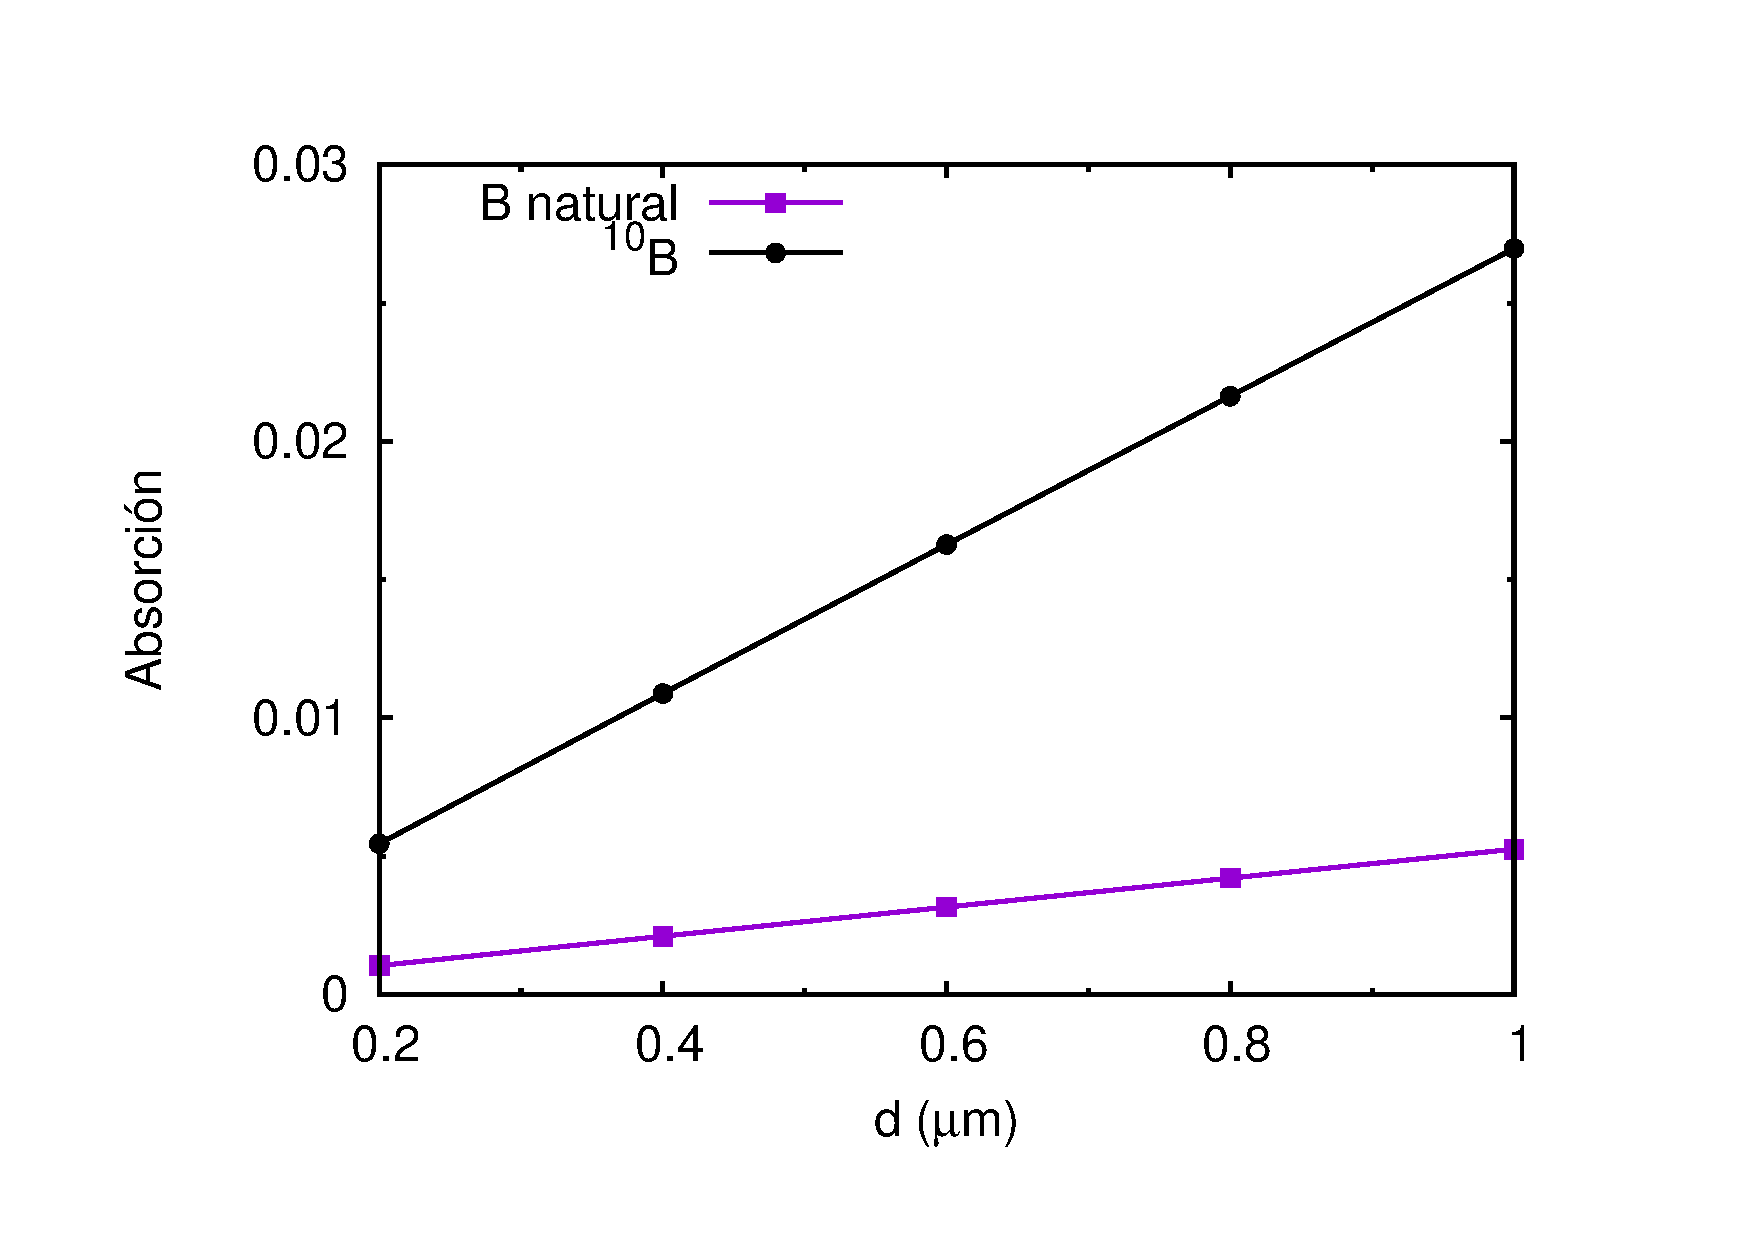
\includegraphics[width=0.9\columnwidth, angle=0]{Avsd_perpendicular}
  \end{center}
  \vspace{-1cm}
  \caption[Variación de la eficiencia del detector de MgB$_2$ en función del espesor del mismo, para un haz que incide perpendicularmente en el film.]{Variación de la eficiencia del detector de MgB$_2$ en función del espesor del mismo, para un haz que incide perpendicularmente en el film. Puede verse que la eficiencia del detector aumenta considerablemente al reemplazar el B natural del superconductor por $^{10}$B, y que es lineal con el espesor del film dentro del intervalo considerado.}
\label{fig:Avsd_perpendicular}
\end{figure}

En la Fig.\,\ref{fig:Avsd_perpendicular} se ve la variación del coeficiente de absorción de neutrones en función del espesor del detector, considerando sólo la sección eficaz de absorción del $^{10}$B. Puede observarse que la eficiencia del detector crece linealmente con el espesor del film, lo cual es razonable ya que dicho espesor es mucho menor que el camino libre medio de un neutrón en el MgB$_2$ ($\lambda_n(\rm MgB_2) \ \approx \ 35$\,$\mu$m). Se verificó además que, en este rango de espesores, la capacidad de absorción del detector se incrementa proporcionalmente con la concentración de $^{10}$B en el detector, lo que también es intuitivamente razonable.

También se calculó la eficiencia del detector suponiendo que el haz de neutrones incide en forma paralela al film de MgB$_2$, lo que supone reducir el área de colección de neutrones pero permite un incremento notable de la eficiencia, ya que ahora el neutrón debe recorrer varias veces el camino libre medio $\lambda_n$ dentro del MgB$_2$, y esto hace que la probabilidad de que ocurra la captura de un neutrón por un núcleo de $^{10}$B se vuelva próxima a 1.
\begin{figure}[h!]
 \vspace{-0.5cm}
  \begin{center}
    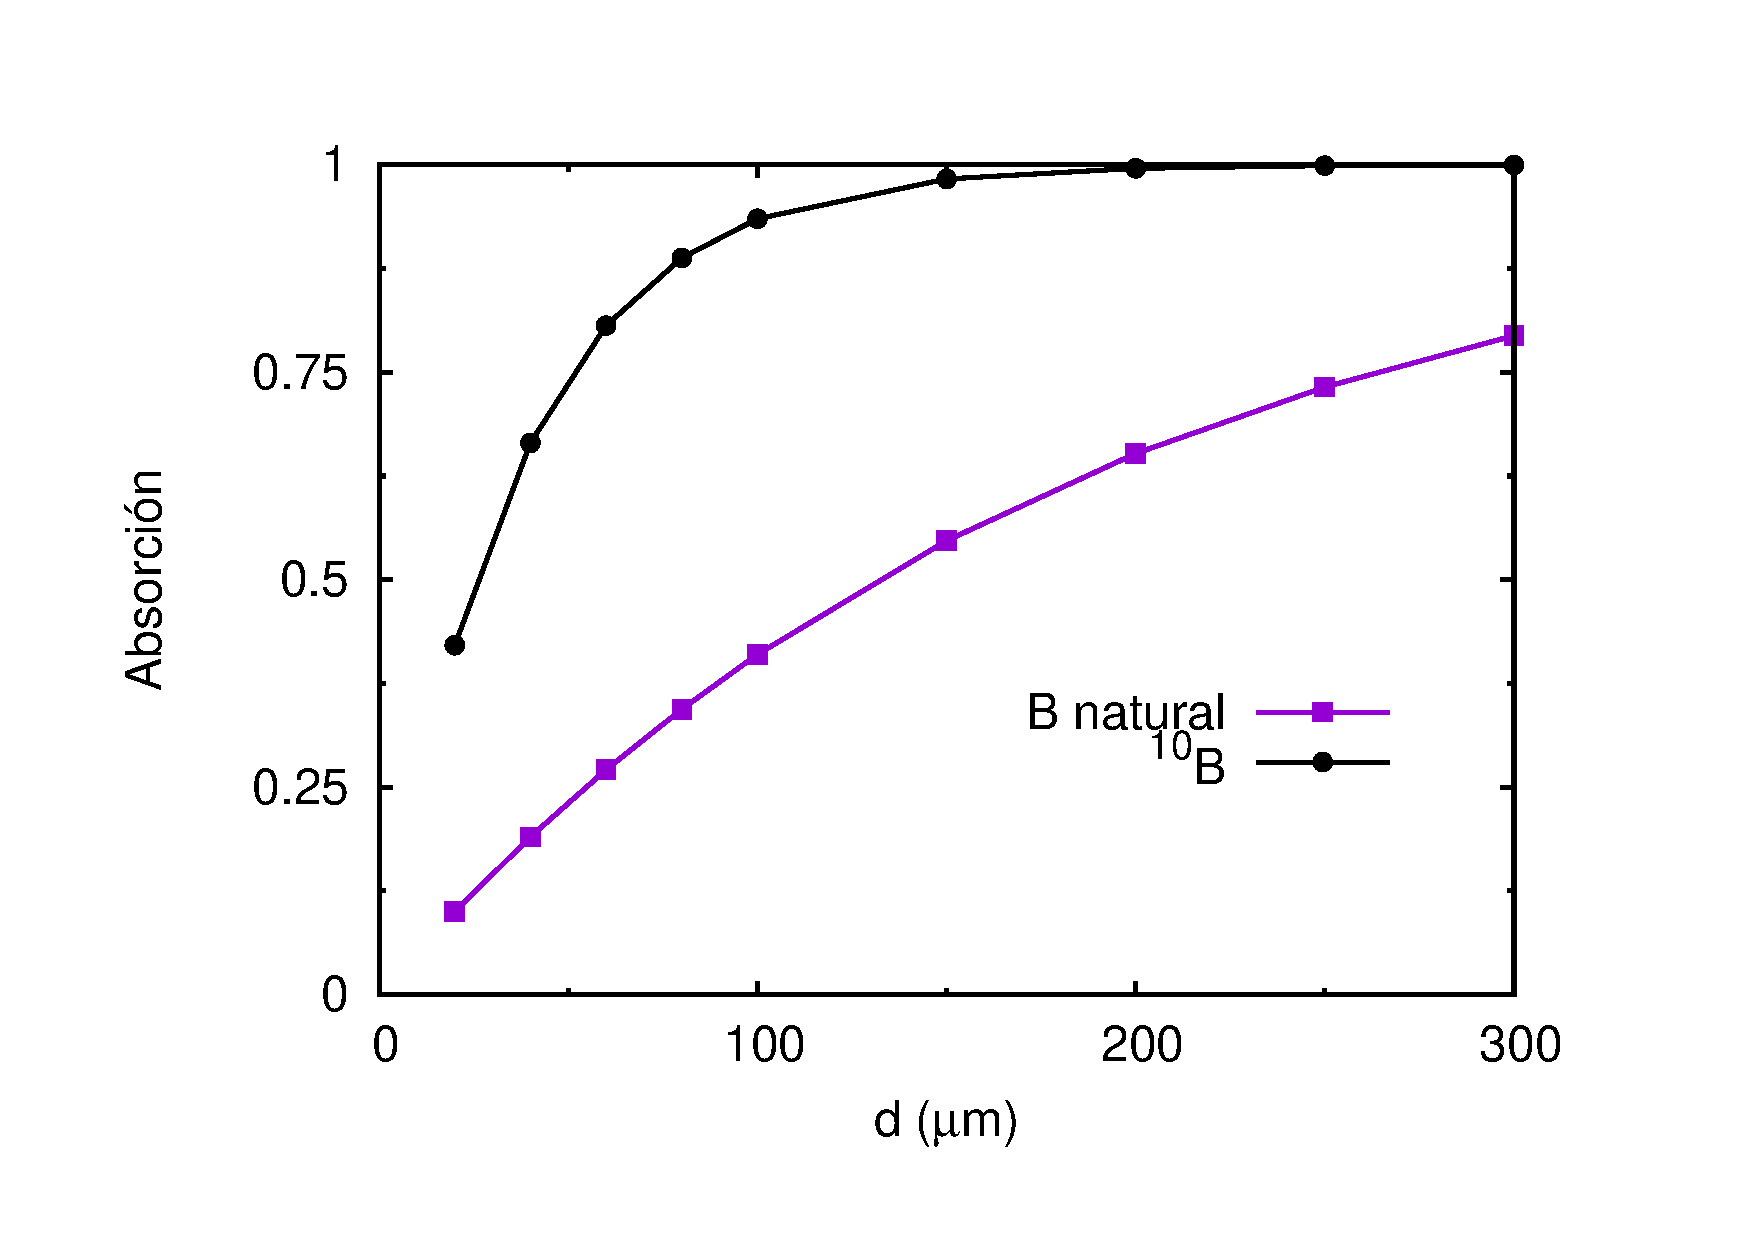
\includegraphics[width=0.9\columnwidth, angle=0]{Avsd_paralelo}
  \end{center}
  \vspace{-1cm}
  \caption[Variación de la eficiencia del detector de MgB$_2$ en función del espesor del mismo, para un haz que incide paralelamente al film.]{Variación de la eficiencia del detector de MgB$_2$ en función del espesor del mismo, para un haz que incide paralelamente al film. En esta configuración, el beneficio que se obtiene al reemplazar el B natural del superconductor por $^{10}$B es mucho menor que el observado en la Fig.\,\ref{fig:Avsd_perpendicular}, cuando el haz neutrones incidía perpendicularmente al film. También se observa que la eficiencia deja de crecer linealmente con el espesor del film y que para un cable de 300\,$\mu$m de longitud, la eficiencia del detector supera el 75\,\%.}
\label{fig:Avsd_paralelo}
\end{figure}

En la Fig.\,\ref{fig:Avsd_paralelo} pueden verse los resultados de calcular la eficiencia del detector para esta configuración.  En esta situación se observa que la eficiencia del detector es mucho mayor que para la configuración anterior y que dicha eficiencia ya no se incrementa linealmente con el espesor, todo lo cual es debido a que ahora el camino que debe recorrer el neutrón en el MgB$_2$ es comparable o mayor a $\lambda_n$. Por otro lado, al incrementarse el volumen de colección en la dirección del haz de neutrones, la eficiencia tiende a 1 y ya no se obtiene un beneficio tan notable al construir el detector utilizando únicamente $^{10}$B. Por último cabe aclarar que aunque esta configuración presenta eficiencias notablemente mayores que las mostradas anteriormente, tiene la desventaja de que permite registrar un número reducido de eventos, ya que ahora el área disponible para la colección de neutrones es muy inferior al caso anterior.

Vale la pena comentar que las eficiencias calculadas en esta sección constituyen un límite superior a la eficiencia real del detector, ya que en este modelo se está teniendo en cuenta que cada captura produce un evento en el detector, lo que no es cierto en general. Si se tiene en cuenta lo discutido en la sección \ref{S:term}, respecto a la estimación del volumen en que se deposita la energía de la reacción, y lo analizado en la sección \ref{S:signal}, respecto a las dimensiones mínimas que debe tener el cable para que se pueda obtener una buena señal a la salida del detector, debe concluirse que las eficiencias calculadas en esta sección son mayores a las efectivamente se deberían observar por lo menos en un factor 3. Esto se debe a que los fragmentos que salen en dirección perpendicular al largo del del cable de MgB$_2$ tienen muy baja probabilidad de depositar su energía en el mismo y escaparán del material.

Cabe mencionar que aunque la eficiencia de este tipo de detectores parece ser muy pobre, son del orden de las que se pueden esperar en los detectores sensibles a posición, tal como el que se planea construir. Esto es así porque cuando se quiere realizar un detector con elevada resolución espacial, es preciso que la energía del evento que se quiere detectar se deposite en una región pequeña del material, tanto más pequeña cuanto más preciso se quiere ser a la hora de definir el lugar en el que ocurrió el evento. Como la eficiencia de detección está relacionada directamente con el volumen de colección que tenga el dispositivo, es de esperar que si se busca resolución en posición, se pierda eficiencia de detección.

\nomenclature{$S$}{Sección eficaz total para la interacción entre un núcleo y un neutrón.}
\nomenclature{$n$}{Número de átomos por unidad de volumen.}
\nomenclature{$\lambda_n$}{Camino libre medio de un neutrón en un material dado.}

%\chapter{Crecimiento de films de MgB$_2$ por evaporación}\label{C:evap}
\graphicspath{{figs/evap/}}

\chapterquote{La vida es como el Tetris, los errores se acumulan y los aciertos desaparecen}{Dicho popular}
%%%%%%%%%%%%%%%%%%%%%%%%%%%%%%%%%%%%%%%%%%%%%%%%%%%%%%%%%%%%%%%%%%%%%%%%
En este capítulo se muestran los resultados obtenidos al intentar fabricar films superconductores de MgB$_{2}$, mediante una técnica que consistió en evaporar films de boro sobre un sustrato, para luego recocer en una ampolla de cuarzo los mismos films junto con una pastilla bulk de MgB$_{2}$ obtenida comercialmente. Los sustratos elegidos fueron zafiro y silicio, dos materiales que poseen una baja conductividad eléctrica y elevada conductividad térmica a bajas temperaturas. El silicio presenta la ventaja adicional de que puede ser fácilmente micromaquinado por procedimientos estándar. Se muestran además mediciones del espesor de los films utilizando un perfilómetro mecánico y la caracterización de las propiedades magnéticas obtenidas a partir de mediciones en un magnetómetro SQUID. La técnica de crecimiento empleada en este capítulo posee la ventaja de ser muy sencilla de implementar pero posee las desventajas de ser un proceso poco repetible que involucra elevadas temperaturas para poder funcionar bien. El mayor problema con los procesos que requieren elevadas temperaturas es que los mismos son más susceptibles a contaminación. Por ejemplo, a altas temperaturas el oxígeno del zafiro puede reaccionar con el magnesio que se quiere depositar en el film de boro, lo que produce un ensanchamiento de la transición superconductora, empeorando el rendimiento del detector.

\section{Procedimiento}\label{S:evapproc}
La fabricación de las muestras por evaporación se realizó en dos etapas: en la primera etapa se evaporó B sobre diferentes sustratos y en la segunda se hizo un recocido de los films evaporados encapsulados junto a muestras bulk de MgB$_2$. Como sustratos se eligieron monocristales de silicio (111) y zafiro (0001). Se utilizaron estos sustratos porque, dentro de los disponibles en el laboratorio, presentan propiedades que interesan para la construcción del detector, básicamente una buena conductividad térmica y son aisladores\cite{Ekin2006}. El objetivo del recocido es colocar a los films de boro en un ambiente en el que estén en equilibrio con la presión de vapor de la muestra bulk de MgB$_2$\cite{Barrabas2011}. En una situación así se busca igualar los potenciales químicos de ambos materiales, lo que implica que los films de boro incorporarán magnesio hasta tener una composición idéntica a la de la muestra bulk. La evaporación de boro sobre el sustrato se hizo en un equipo como el que se esquematiza en la Fig.\,\ref{fig:eva}.
\begin{figure}[tbh!]
 \begin{center}
    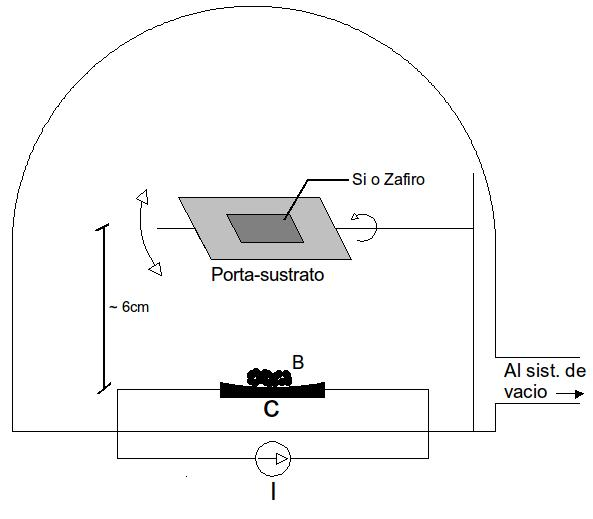
\includegraphics[width=0.6\columnwidth]{evaporadora1}
  \end{center}
  \caption[Esquema del arreglo utilizado para evaporar boro sobre diferentes sustratos.]{Esquema del arreglo utilizado para evaporar boro sobre diferentes sustratos. I es la fuente de corriente
que se utilizó para hacer pasar corriente sobre la naveta C, sobre la que depositó el boro. El interior de la campana se encontraba en condición de alto vacío ($P \sim 10^{-6}$\,Torr).}
\label{fig:eva}
\end{figure}
%\newpage
El boro se evaporó desde una naveta de grafito tallada especialmente (Fig.\,\ref{fig:nav}). Las navetas se angostaron de modo de aumentar la densidad de corriente en el centro de la misma, y se pusieron en serie con una fuente de corriente que podía entregar hasta 150\,Ampere. El sustrato se colocó en el porta-sustrato y se ubicó por sobre la naveta. El depósito de boro se hizo en condiciones de alto vacío ($p$ $\sim$ $10^{-6}$\,Torr).
\begin{figure}[tbh!]
 \begin{center}
    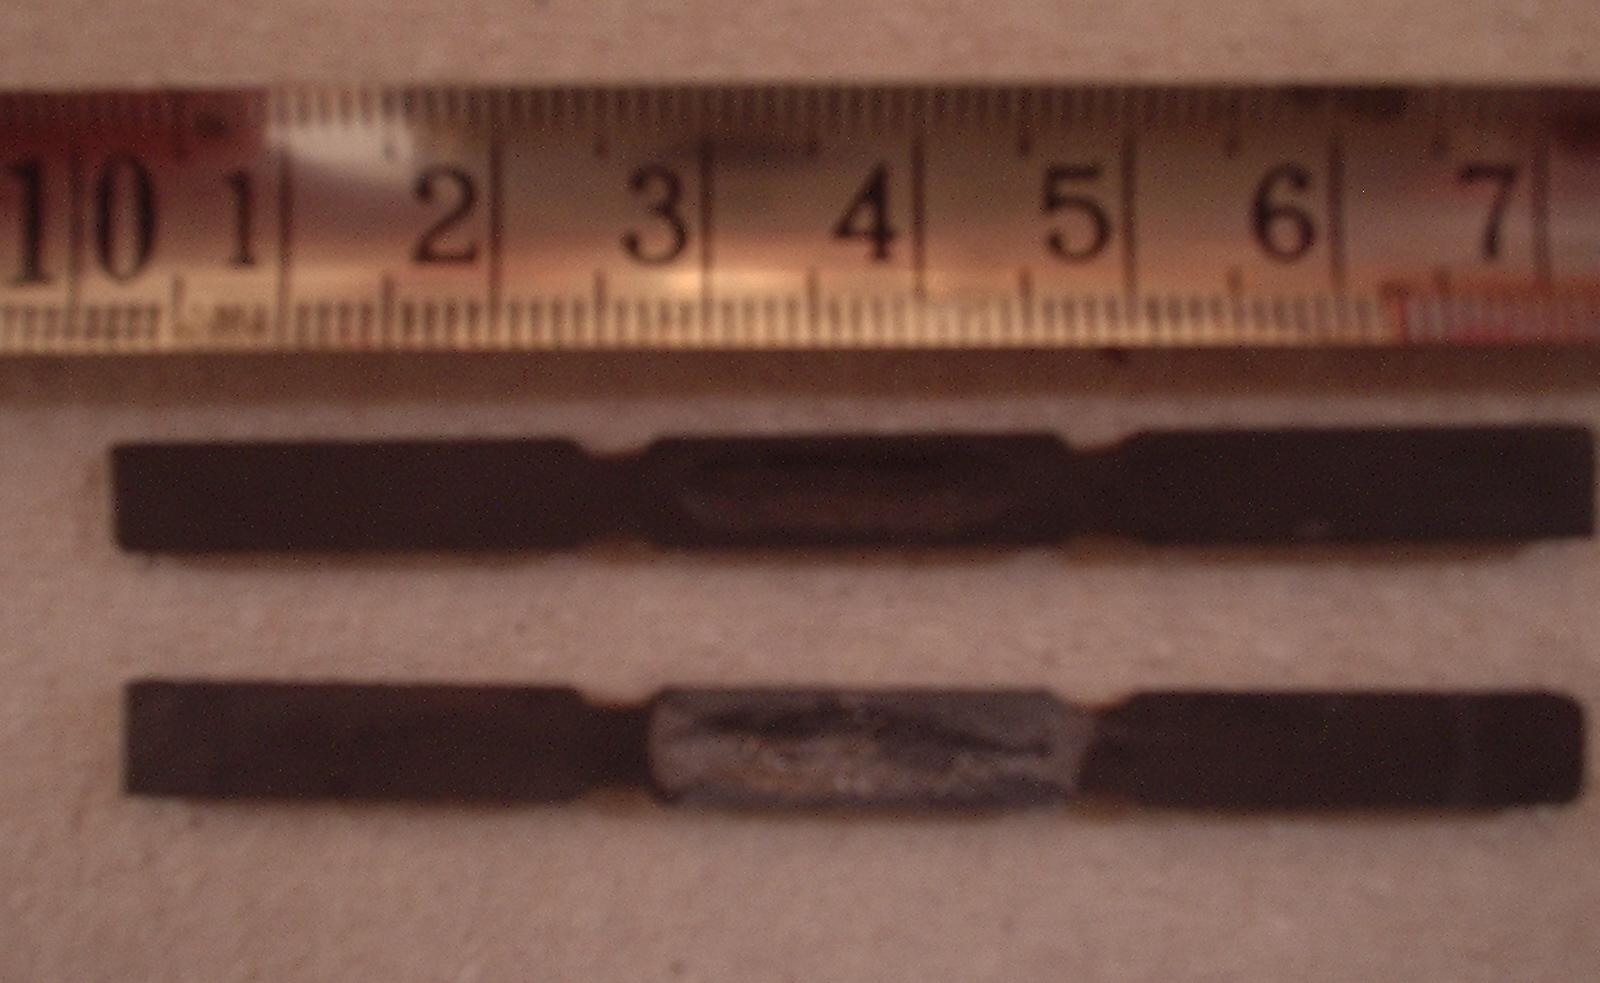
\includegraphics[width=0.5\columnwidth]{navetas}
  \end{center}
  \caption[Las navetas de grafito utilizadas para la evaporación.]{Las navetas de grafito utilizadas para la evaporación. Las mismas fueron talladas especialmente
de modo de incrementar la densidad de corriente en las regiones en las que se depositaba el boro. Puede apreciarse
la diferencia de cómo se veían las navetas antes de la evaporación (arriba) y después de la misma (abajo).}
  \label{fig:nav}
\end{figure}
\nomenclature{$p$}{Presión hidrostática.}
\newpage
Una vez crecidos los films, se colocaron en un tubo de cuarzo junto con una pastilla de MgB$_2$ envuelta en una lámina de tantalio, como se ve en la Fig.\ref{fig:tubos}. El tantalio evita la oxidación de los films, ya que absorbe el oxígeno que desgasa la pastilla de MgB$_2$ durante el recocido\cite{Barrabas2011}.
El tubo de cuarzo así sellado se colocó en un horno donde se realizó el recocido a diferentes temperaturas y por diferentes períodos de tiempo, alrededor de los 700 ºC y las 20 hs, respectivamente.
\begin{figure}[tbh!]
 \begin{center}
    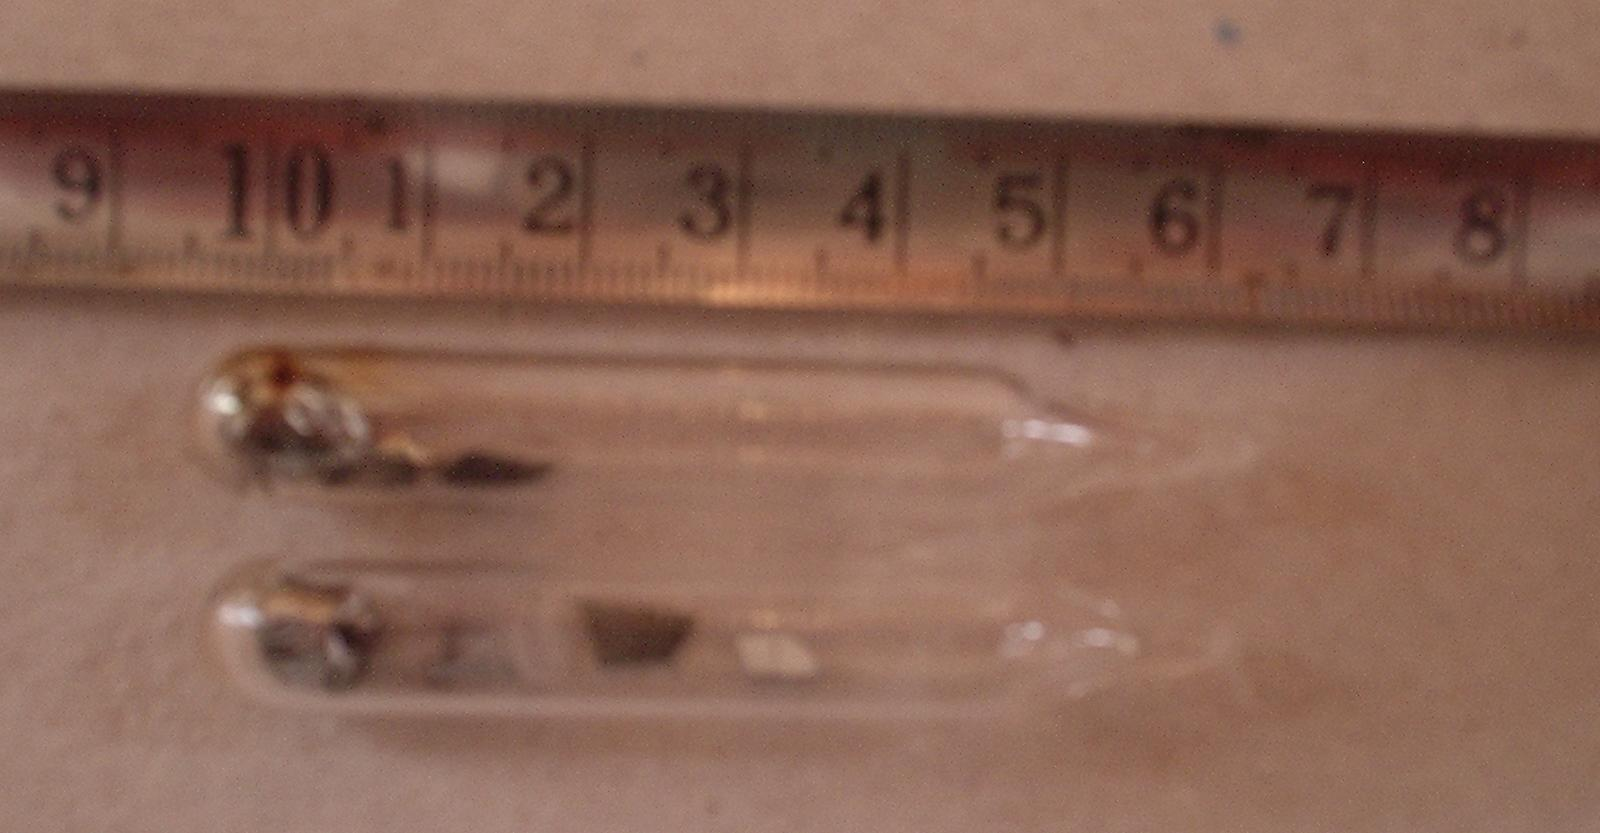
\includegraphics[width=0.5\columnwidth]{tubos}
  \end{center}
\caption[Tubos de cuarzo utilizados para recocer los films de boro con pastillas de MgB$_2$.]{Tubos de cuarzo utilizados para recocer los films de boro con pastillas de MgB$_2$. El MgB$_2$ fue envuelto 
en una lámina de tantalio para evitar la oxidación de los films.}
\label{fig:tubos}
\end{figure}

Los films obtenidos fueron caracterizados en un magnetómetro SQUID en donde se midió su magnetización en función de la temperatura durante un proceso \textit{Zero field cooling - Field cooling} (ZFC-FC). El SQUID es un dispositivo que consiste en un arreglo de junturas Josephson que permiten medir campos magnéticos con elevada precisión y bajos niveles de ruido, por lo que resulta un equipo muy útil para determinar la magnetización de films, que son materiales con masas pequeñas, y que por ende producen señales magnéticas también pequeñas. El proceso ZFC-FC consiste en llevar al superconductor a una temperatura $T\ < \ T_{c}$, a campo nulo, para luego aplicar un campo magnético $H \ < H_c$ (proceso \textit{Zero Field Cooling}). Como en el interior de un superconductor se tiene $B\ = \ 0$, el SQUID registra una señal diamagnética que proviene de la muestra, es decir que se tiene $M \, < \, 0$. El paso siguiente del proceso es calentar el sistema, con campo aplicado, hasta que se tiene $T \ > \ T_c$, lo que lleva al material al estado normal. Es esta circunstancia, el campo magnético penetra en el superconductor y el SQUID registra una señal nula, o sea, $M \ = \ 0$. El paso final del proceso consiste en enfriar nuevamente a $T \ < \ T_c$ con campo aplicado (proceso \textit{Field Cooling}). Sin embargo, como el campo ya penetró en el material, cuando se cumple $T \ < \ T_c$, la expulsión del campo magnético no es completa, lo que implica que se observa una irreversibilidad en el gráfico $M \ vs \ T$ cuando el superconductor es sometido a un proceso ZFC-FC.
\nomenclature{$H$}{Campo magnético aplicado.}

La medición de magnetización en un proceso de este estilo es una técnica estándar utilizada para la determinación del carácter superconductor de un film, así como un método muy preciso para determinar su $T_{c}$.

El ciclo ZFC-FC elegido para caracterizar las muestras consistió en llevar la muestra a 5\,K a campo nulo y aplicar un campo magnético. A continuación se incrementó lentamente la temperatura de la muestra hasta $T \ = 45$\,K, que es una temperatura mayor que la mayor $T_c$ esperable para el MgB$_2$. Luego se enfrió nuevamente la muestra hasta $T\ = 5$\,K con campo aplicado. En la Fig.\,\ref{fig:bulk} se muestra, a modo de ejemplo, la curva de magnetización de la pastilla de MgB$_2$ utilizada para generar los films.
\begin{figure}[tbh!]
 \begin{center}
    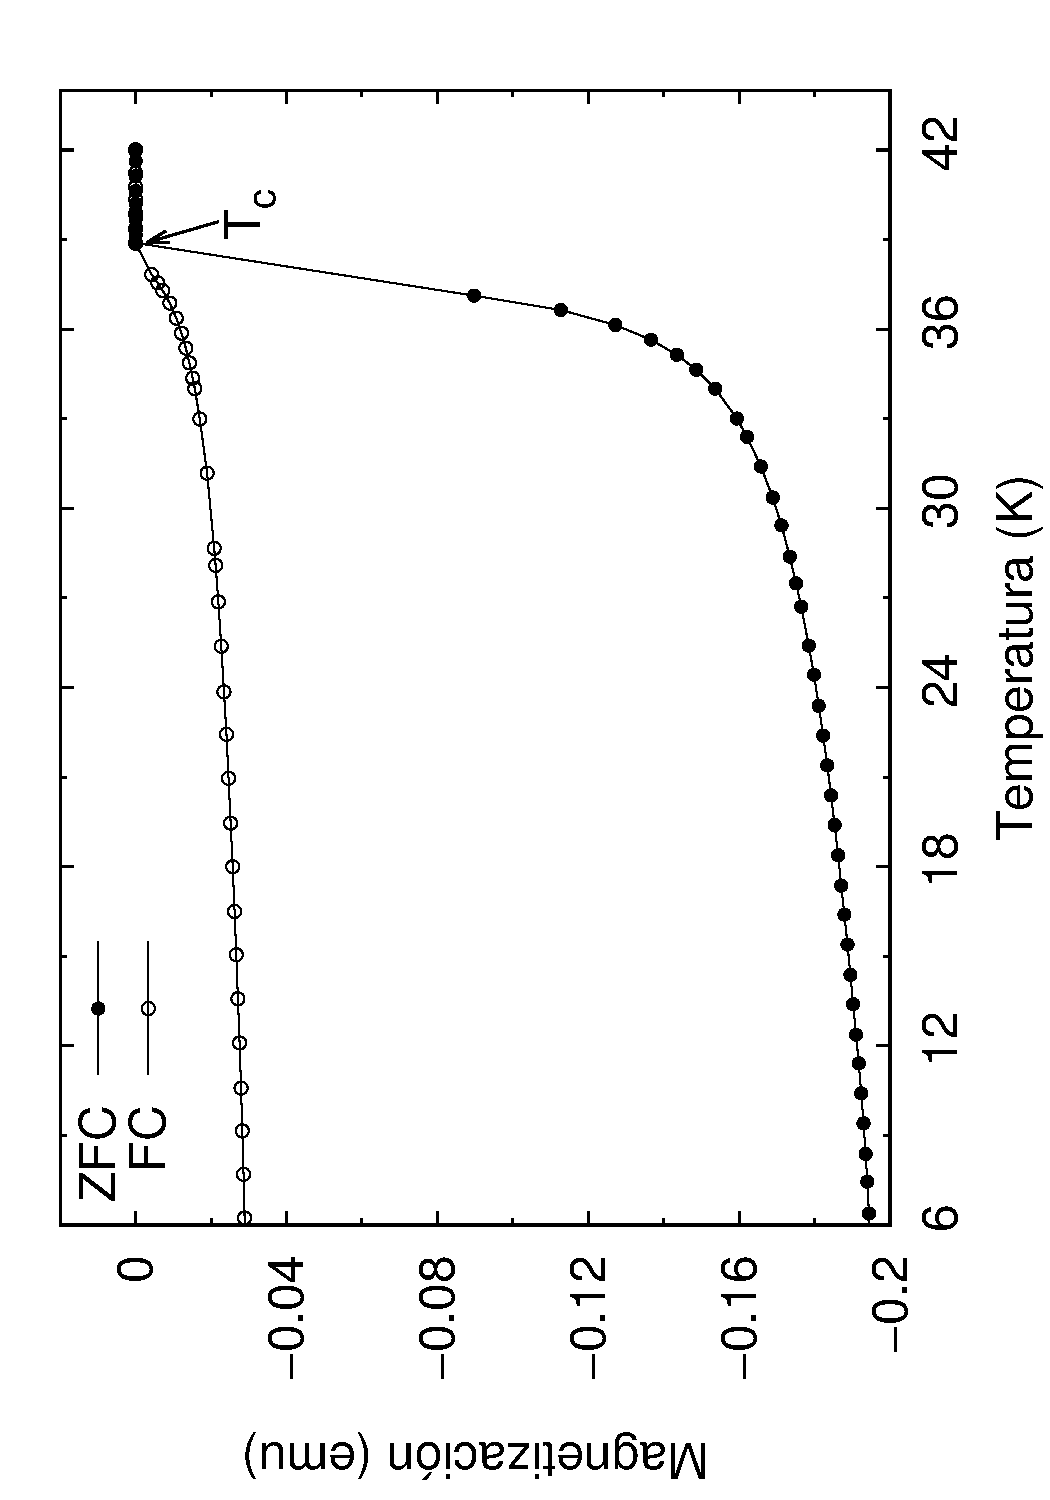
\includegraphics[width=0.5\columnwidth, angle=-90]{mgb2bulk}
  \end{center}
\caption{Curvas de magnetización en un proceso ZFC-FC de la pastilla de MgB$_2$ utilizada para generar los films.}
\label{fig:bulk}
\end{figure}
%\newpage
En este trabajo se realizaron tres evaporaciones con sus correspondientes recocidos: la primera con sustratos del silicio y las otras dos con sustratos de silicio y zafiro. Las muestras de la segunda evaporación se recocieron mezclando en el tubo de cuarzo muestras con sustratos de silicio y zafiro y las de la tercera recociendo por separado el zafiro y el silicio. Las muestras de la primera evaporación estaban muy contaminadas y no resultaron ser superconductoras.

\section{Caracterización de los films de MgB$_2$}\label{S:evapcarac}
Se presenta a continuación la caracterización realizada sobre las distintas muestras fabricadas. Tal como se comentó previamente, los films de la primera evaporación estaban demasiado contaminados y, debido a eso, no eran superconductores. En la tabla\,\ref{tab:muestras} se muestran resumidos los datos obtenidos de las distintas muestras. Sólo aparecen los datos de la segunda y la tercera evaporación.
\begin{table}[h!]
\centering
\begin{tabular}{|c|c|c|c|c|c|} \hline
  N$^{\circ}$ de Evap.& Muestras & Sustrato & $T_{rec}$(C) & $t_{rec}$(hs.) & Espesor (nm) \\ \hline
2 & BBSi 1 a 4&Si (111)&750&20&$(540 \, \pm \, 50)$ \\
2 & BBZ 1 a 3&Al$_2$O$_3$ (0001)&750&20&$(540 \, \pm \, 50)$  \\ \hline
3 & BBSi 5 a 9&Si (111)&700&20&$(80 \, \pm \, 10)$ \\
3 & BBZ 4 a 8&Al$_2$O$_3$ (0001)&700&20&$(80 \, \pm \, 10)$\\ \hline
\end{tabular}
\caption[Las muestras producidas por medio del método de evaporación y recocido.]{Las muestras producidas en esta etapa del trabajo. Se muestran los tiempos y temperaturas de los recocidos,
el sustrato en el que fueron crecidas las muestras y el espesor estimado de las mismas.}
\label{tab:muestras}
\end{table} 

A modo de ejemplo, se muestran en las Figs.\,\ref{fig:mgb2si} y \ref{fig:mgb2zaf} curvas representativas de magnetización en función de la temperatura para dos de las muestras fabricadas, una depositada sobre sustrato de silicio y otra sobre sustrato de zafiro. La curva de magnetización en función de la temperatura del film BBSi 3 aparece en la Fig.\,\ref{fig:mgb2si}.
\begin{figure}[h!]
 \begin{center}
    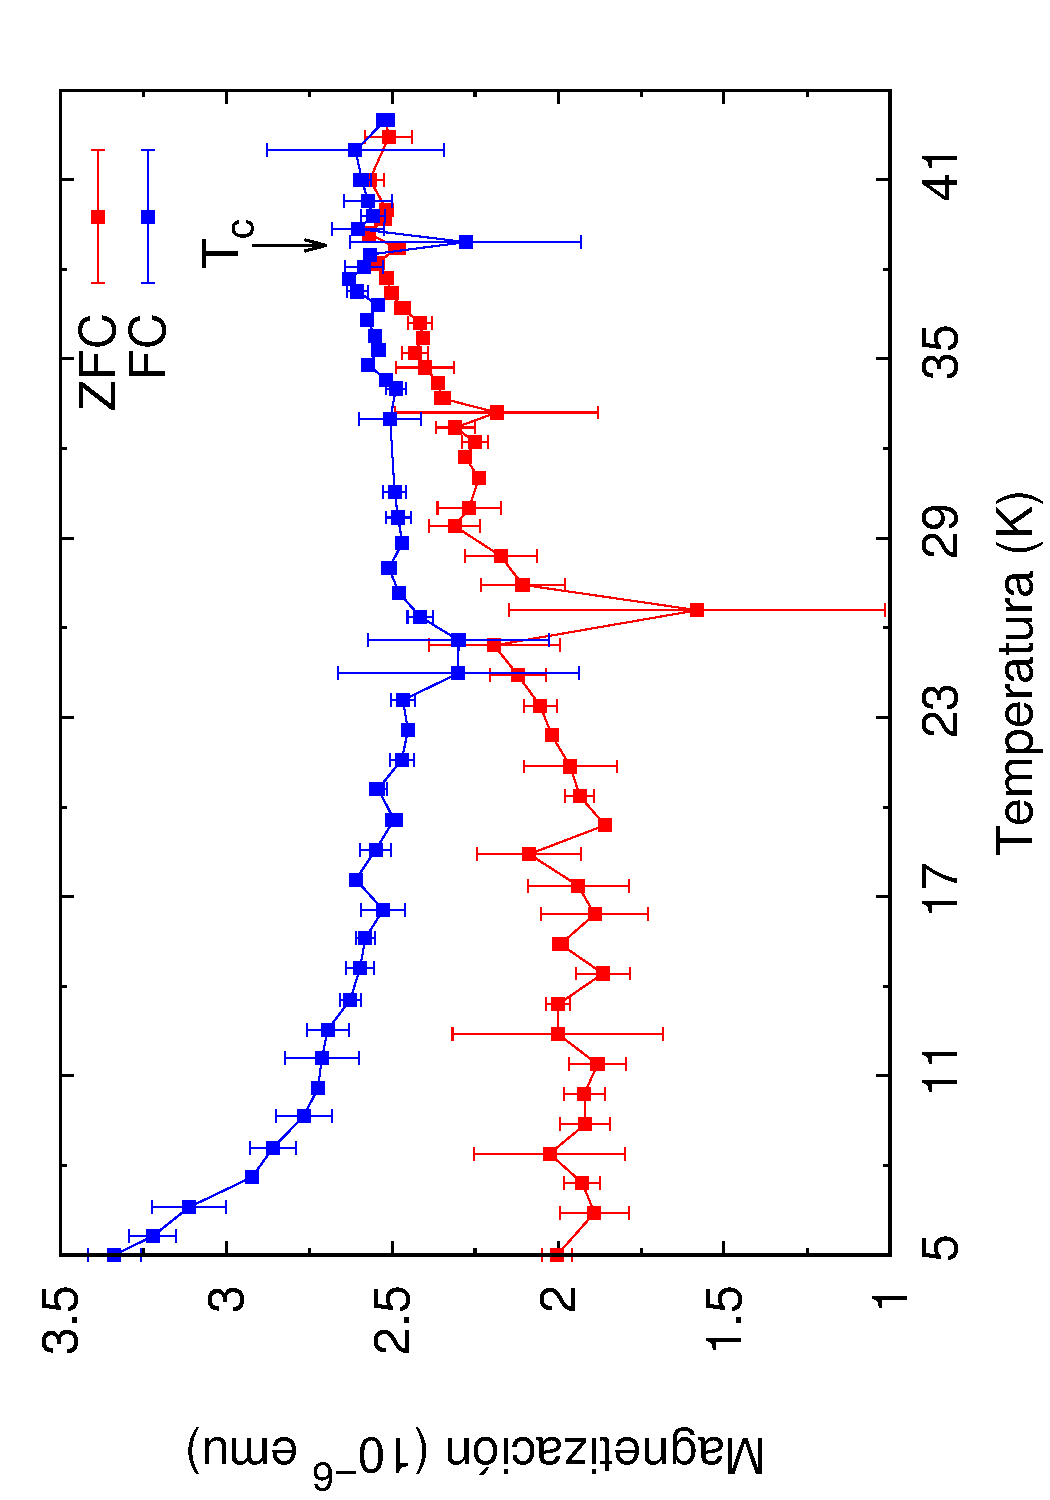
\includegraphics[width=0.5\columnwidth, angle=-90]{mgb2si}
  \end{center}
\caption[Magnetización en función de la temperatura para la muestra BBSi 3.]{Magnetización en función de la temperatura para la muestra BBSi 3. El sustrato es de Si. El hecho de que la señal sea positiva se debe al paramagnetismo del silicio. Sin embargo puede apreciarse una irreversibilidad que indica una transición superconductora cuya $T_c$ se encuentra entre 36\,K y 38\,K.}
\label{fig:mgb2si}
\end{figure}
\newpage
Puede verse que la curva de magnetización de la figura\,\ref{fig:mgb2si} es cualitativamente si\-mi\-lar a la obtenida al medir la pastilla de MgB$_2$ utilizada para hacer el recocido de los films (ver Fig.\,\ref{fig:bulk}). La irreversibilidad de la curva de magnetización sugiere que existe una transición superconductora a una $T_c$ algo menor que 38\,K. El hecho de que la señal sea positiva se debe al paramagnetismo del sustrato de Si\cite{Barrabas2011}.
\begin{figure}[h!]
 \begin{center}
    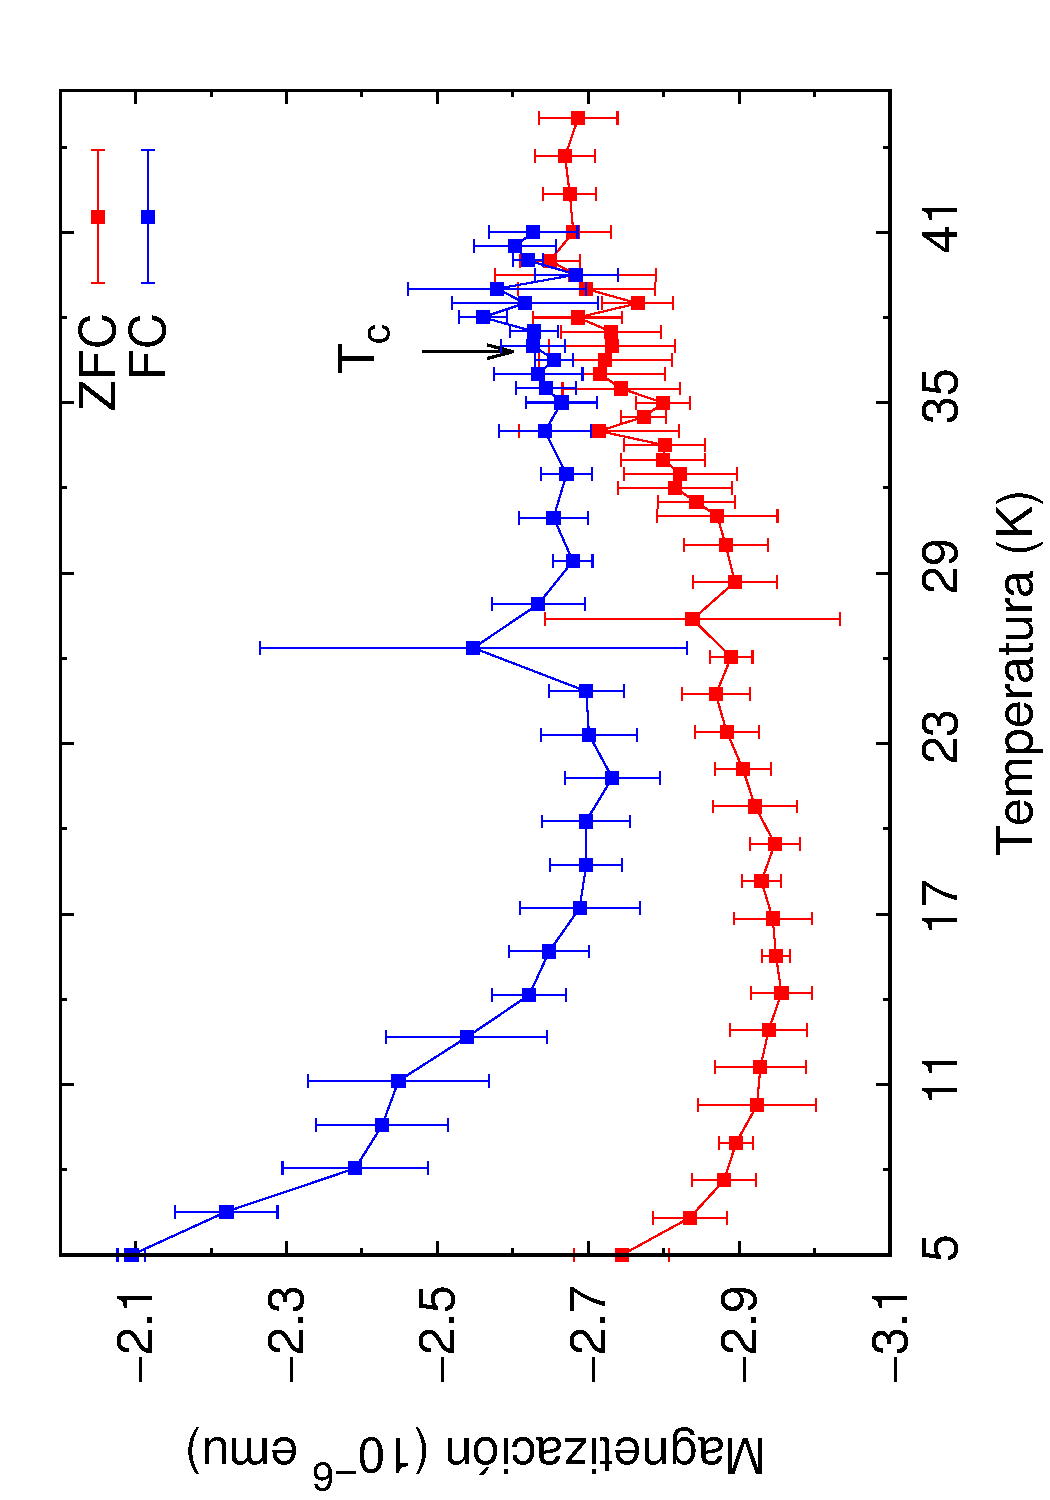
\includegraphics[width=0.5\columnwidth, angle=-90]{mgb2zaf}
  \end{center}
\caption[Magnetización en función de la temperatura para la muestra BBZ 1.]{Magnetización en función de la temperatura para la muestra BBZ 1. El sustrato es de zafiro. Al comparar con la Fig.\,\ref{fig:mgb2si}, puede apreciarse que en este caso la magnetización es negativa, y que la $T_c$ de este film también está entre 36\,K y 38\,K. Esto último es razonable, ya que ambas muestras fueron recocidas juntas.}
\label{fig:mgb2zaf}
\end{figure}

La figura\,\ref{fig:mgb2zaf} muestra la magnetización para un film de MgB$_2$ depositado sobre un sustrato de zafiro. Se aprecia una curva similar a la de la Fig.\,\ref{fig:mgb2si} aunque con magnetización negativa. Esto confirma la idea de que en el caso anterior, la magnetización positiva se deba al sustrato de Si.

También se midió el espesor de los films crecidos utilizando un perfilómetro mecánico de aguja. En la figura\,\ref{fig:histo2} se muestran las mediciones realizadas para la muestra BBZ 7. Para medir el espesor de los films se colocó pintura de plata en el sustrato antes de hacer la evaporación, y una vez realizada la misma, se removió la pintura, dejando expuesto un escalón que iba a permitir medir el espesor del film crecido. Luego se llevó la muestra cuyo espesor se deseaba determinar al perfilómetro mecánico, un equipo que consiste en una aguja que se puede mover en el plano de la muestra (plano xy), y que registra las variaciones en el eje perpendicular a ese plano (eje z) a partir de medir el desplazamiento vertical de la agua usando un sensor magnético. De las mediciones en el perfilómetro se obtuvieron perfiles como el que se ve en la Fig.\ref{fig:histo2}. Para cada muestra, se obtuvieron los perfiles de los escalones en diferentes lugares, y el espesor de los films se estimó de la siguiente forma: se ajustó una recta a cada nivel del escalón y luego se midió la distancia vertical entre dichas rectas en un punto del escalón. Se midió el espesor de los films antes del recocido y después de realizar el mismo. A partir de estas mediciones se estimó que la altura de los films de la 3ª evaporación tienen un espesor $d \, \approx \, 80 $\,nm, después de realizado el recocido. Mediciones análogas determinaron que la altura de los films de la 2ª evaporación es $d \, \approx \, 550 $\,nm, también después del recocido.

\begin{figure}[h!]
 \begin{center}
    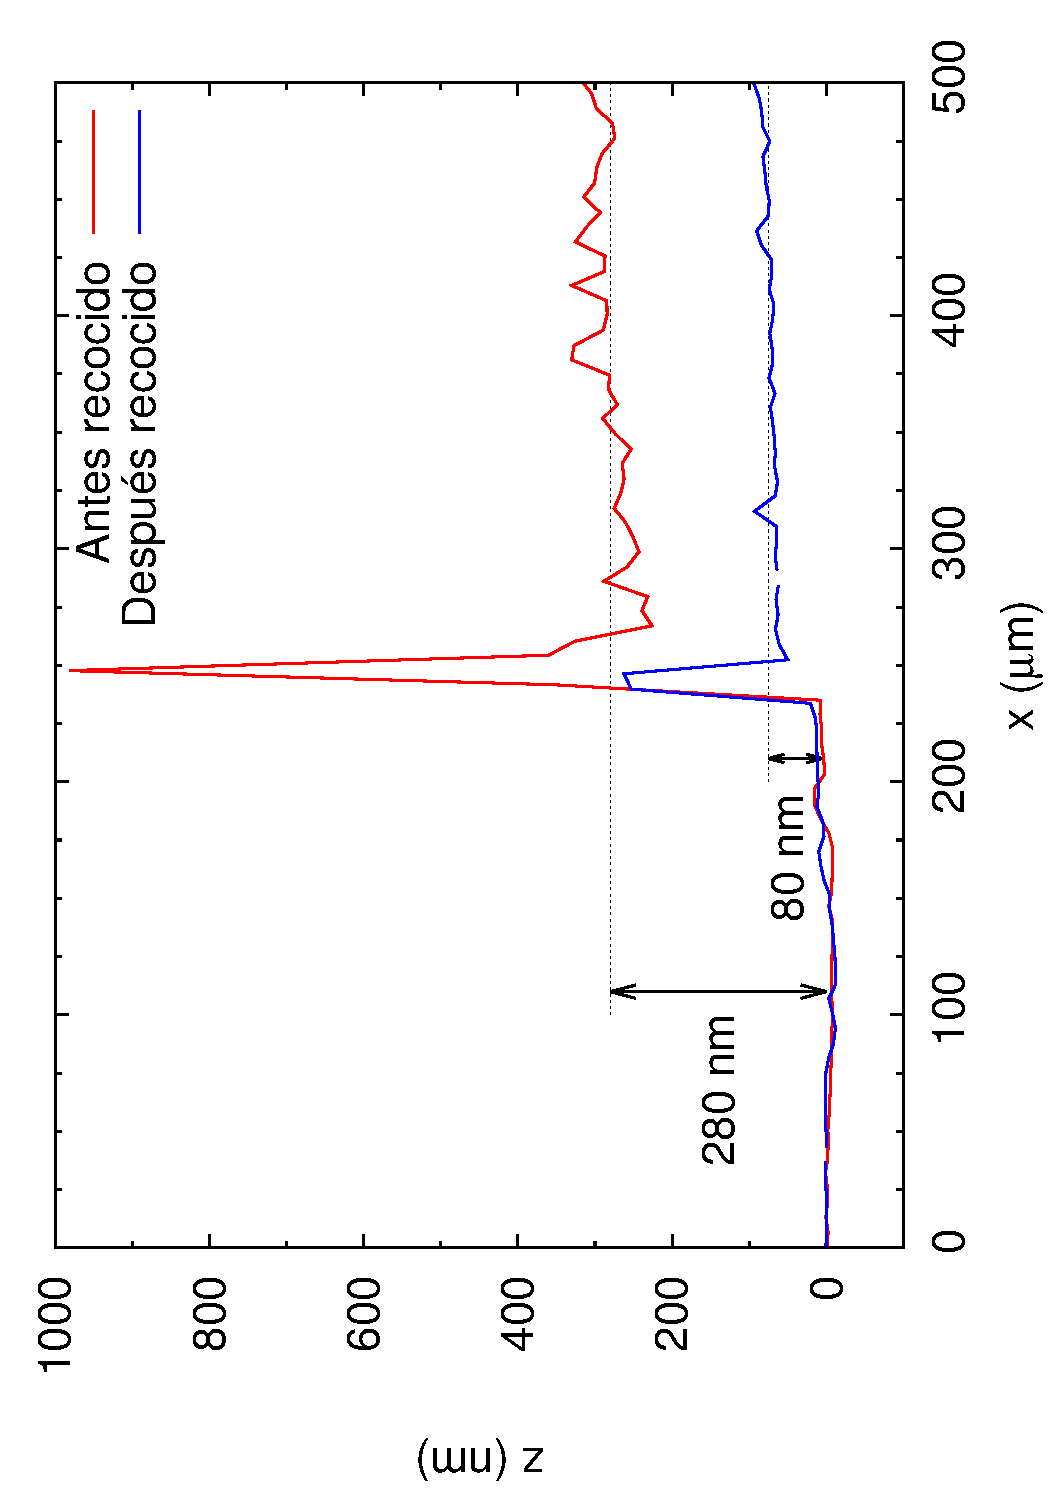
\includegraphics[width=0.5\columnwidth, angle=-90]{altura}
  \end{center}
\caption[Altura de los films de boro (antes del recocido) y de los MgB$_2$ (después del recocido).]{Altura de los films de boro (antes del recocido) y de los MgB$_2$ (después del recocido). Puede verse claramente que el espesor de los films disminuye notablemente después del recocido.}
\label{fig:histo2}
\end{figure}
%\newpage
En la Fig. \ref{fig:histo2} se compara la medición de la altura de la muestra BBZ 7 antes de realizar el recocido y después de realizar el mismo, lo que permite notar que los films se vuelven muchos más delgados después de ser recocidos. Se pensó que esto podía deberse a que parte del MgB$_2$ de la pastilla se depositaba en la parte descubierta del sustrato, lo que implicaría que la disminución del espesor del film es sólo aparente. En caso de ser cierto este supuesto, cabe entonces hacer la pregunta de si la irreversibilidad observada en las Figs \ref{fig:mgb2si} y \ref{fig:mgb2zaf} no es debida al MgB$_2$ que se depositó sobre los films. Para verificar esta hipótesis, se creció un film de boro con dos máscaras, una que se quitó antes del recocido y otra que se quitó después. Al hacer esto se pudo apreciar que es correcto pensar que algo del MgB$_2$ se deposita en el sustrato, pero lo que se deposita no es suficiente como para explicar la disminución observada en el espesor del film. Por otro lado se pensó que esta variación de alturas podía deberse a la diferencia de densidades del boro y el MgB$_2$, pero esta variación tampoco alcanza para explicar las variaciones medidas.

Investigando en la literatura que se encontró que es posible que debido a las altas temperaturas del recocido, parte del film difunda a través del sustrato \cite{Zhai1995, Naito2004, He2002}. En \cite{He2002} se muestra como el oxígeno presente en el zafiro reacciona con el Mg a temperaturas mayores a 600\,$^{\circ}$C, y esto resulta en una transición superconductora ancha. En el mismo trabajo también se muestra que el recocido con silicio da resultados parecidos.

\section{Análisis del método}\label{S:evapanalisis}
El método de evaporación y recocido realizado en este trabajo presenta como principal punto positivo el de que emplea un equipo relativamente sencillo de utilizar. Además, la $T_{c}$ de los films obtenidos no parece ser mucho peor que la de pastilla de MgB$_{2}$ utilizada para hacer los recocidos. Sin embargo, el método implementado en esta sección presenta algunos inconvenientes que deben ser tenidos en cuenta si se busca producir un dispositivo electrónico, siendo el primero la pobre adherencia que tienen los films con el sustrato, incluso después del recocido. Esto se debe a que los átomos de boro que se evaporan llegan al sustrato con una energía cinética del orden de la temperatura a la que se encuentra la naveta durante el crecimiento del film, es decir, algunas décimas de eV. Esto resulta en que el átomo que llega no posee la energía suficiente como para explorar el sustrato y acomodarse en la mejor región del mismo, y esto tiene como consecuencia que la adherencia entre el sustrato y el film no sea buena. El siguiente punto negativo es que para poder evaporar boro, se requiere poder calentar el mismo a temperaturas del orden de los miles de grados, y esto sólo se puede lograr utilizando una naveta de grafito, lo que introduce una fuente adicional del contaminación al proceso de crecimiento. Adicionalmente, el procedimiento experimental que hay que seguir para crecer los films no es del todo repetible de crecimiento a crecimiento. Se puede dar como ejemplo el recubrimiento de boro observado en las navetas de grafito (Fig. \ref{fig:nav}), que podía formarse o no, dependiendo de que tan rápido se caliente la naveta durante la evaporación. Por último, las altas temperaturas necesarias para el recocido llevan a que el MgB$_{2}$ que se pretende formar reaccione con el sustrato o difunda a través de él, y esto trae aparejado un ensanchamiento de la transición superconductora. Entonces, si se busca desarrollar un dispositivo electrónico es preciso evitar el paso de recocido o bajar la temperatura a la que ocurre el mismo, así como es necesario un método de depósito que sea más fácilmente reproducible y que permita lograr un film con mejor adherencia. En la sección siguiente se explora la posibilidad de crecer films de MgB$_{2}$ directamente por sputtering, un método que permite lograr films que tienen una excelente adherencia con el sustrato, gracias que las partículas llegan al sustrato con energías del orden los eV. 

%\chapter{Crecimiento de films de MgB$_2$ por sputtering}\label{C:sput}
\graphicspath{{figs/sput/}}
\chapterquote{La vida es como el Tetris, si no cometes errores es que estás desperdiciando oportunidades.}{Corolario del dicho anterior}
%%%%%%%%%%%%%%%%%%%%%%%%%%%%%%%%%%%%%%%%%%%%%%%%%%%%%%%%%%%%%%%%%%%%%%%%
En este capítulo se describen los avances que se han hecho en la búsqueda de crecer films de MgB$_{2}$ directamente por sputtering, esto es, se buscó crecer el material deseado en un sólo paso, tratando de evitar el proceso de recocido. La ventaja de este método, además de evitar el recocido, es que es altamente reproducible, limpio y es capaz de producir films con buena adherencia. La técnica consiste en impactar un blanco del material que se desea depositar (en este caso MgB$_{2}$) con iones de Ar que son acelerados por una diferencia de potencial $V$, de modo de arrancar partículas del mismo blanco para que luego se depositen sobre el sustrato. Como los iones transfieren su energía cinética a las partículas que son arrancadas del blanco, las mismas llegan al sustrato con energías que son del orden de los eV. De esta manera, los átomos que se depositan tienen energía suficiente como para explorar el sustrato de modo de ubicarse en lugar donde la energía de vínculo entre el sustrato y la partícula depositada es máxima. Como se dijo antes, esto implica la posibilidad de hacer films con elevada adherencia.

La ventaja de producir un film in situ, es decir, evitando el proceso de recocido, es que de esta forma se impide que el sustrato y el film reaccionen entre si, lo que contribuye a lograr una transición superconductora abrupta, tal como se requiere para la fabricación del detector.

El trabajo de crecimiento por sputtering fue realizado en el nuevo edificio de Nanociencia y Nanotecnología del Centro Atómico Bariloche, una obra que concluyó durante segundo semestre de la realización de este trabajo. En el mismo semestre se trasladaron las máquinas de sputtering y todos los equipos relacionados con los procesos de microfabricación, que estaban en el Laboratorio de Bajas Temperaturas del mismo Centro Atómico. Esto llevó a que el trabajo de crecimiento de films de MgB$_2$ por sputtering que se muestra en este capítulo, pudiera realizarse solamente en el tercer semestre de trabajo de esta tesis.
%\newpage
\section{Procedimiento}\label{S:sputproc}
Para el crecimiento de films por sputtering se utilizaron sustratos de zafiro (0001) que se pegaron a un calefactor con pintura de plata y un blanco de MgB$_2$ que fue adquirido comercialmente. Se eligió utilizar un sustrato de zafiro por las mismas razones mencionadas en el capítulo \ref{C:evap}. La realización de los depósitos se inició haciendo vacío con una bomba mecánica y encendiendo luego una turbomolecular, con la que se hizo vacío hasta llegar a una presión del orden de $10^{-6}$\,Torr. Luego se calentó el sustrato hasta la temperatura de crecimiento T$_{crec}$ deseada y se lo mantuvo en dicha temperatura por una hora, al mismo tiempo que se hacía circular Ar dentro de la cámara. Se llevó a cabo este procedimiento porque se notó que al calentar el sustrato la presión en la cámara se incrementaba, probablemente debido al desgase del sustrato y de la pintura de plata que se utilizó para pegar el mismo sustrato al calefactor. Una vez purgado el sistema se lograba una presión base para los depósitos de 1\~-\~3\,$\times$10$^{-6}$\,Torr. Durante la realización de este trabajo se variaron diferentes parámetros pertinentes al crecimiento de films, a saber, T$_{crec}$, presión de Ar y potencia aplicada al blanco.

La velocidad de crecimiento del film $v_{crec}$ es proporcional al número de iones Ar que impactan en el blanco y a un coeficiente $Y$ denominado sputtering yield, que indica cuántos átomos del blanco son arrancados cada vez que impacta un ion en el mismo. Ahora bien, el número de iones que impactan en el blanco es directamente proporcional a la corriente que circula por el mismo, mientras que el sputtering yield es una función no lineal de la energía con la que los iones colisionan con el material. Sin embargo, si la energía cinética $K$ de los iones al momento de la colisión es suficientemente baja, se observa experimentalmente que $Y$ es proporcional a la misma. Por otro lado, la energía cinética de los iones va a ser directamente proporcional a la tensión aplicada al blanco, a partir de lo cual se puede concluir que, si la tensión aplicada es lo suficientemente baja (menor a 10$^4$\,V), se tiene que $Y \ \varpropto \ K \varpropto \ V$. Juntando este resultado con el hecho de que el número de iones que impactan en el blanco es proporcional a la corriente $I$ se tiene que:
\begin{equation}
v_{crec} \ \varpropto \ I \ Y \ \varpropto \ I \ V \ = \ P
\label{eq:vcrec_2}
\end{equation}
\noindent
siendo $P$ la potencia aplicada al blanco. El equipo de sputtering utilizado en este trabajo permite controlar la potencia que se aplica al blanco, es decir, que permite controlar que la velocidad de crecimiento sea constante.
\nomenclature{$K$}{Energía cinética.}
\nomenclature{$P$}{Potencia eléctrica.}
\nomenclature{$Y$}{Sputtering yield.}
%\newpage

La temperatura del sustrato se controló con un calefactor y un controlador PID. La temperatura se midió con una termocupla que censaba la base del calefactor. Para estimar la diferencia de temperatura entre la termocupla y la superficie del sustrato se supuso que la termocupla está acoplada perfectamente a la base del sustrato. Pensando que el sistema llegó a un estacionario se estimó la diferencia de temperatura a partir de la expresión\cite{incropera}:
\begin{equation}
	\Delta T \ = \frac{d_s\,\dot{q}}{A_s\,\kappa} \ \sim \ 5\,\mathrm{ºC}
	\label{eq:conduccion}
\end{equation}
\noindent
En este caso $d_s$ es el espesor del sustrato ($\sim$ 0.05\,cm), $A_s$ es el área del mismo ($\sim$\,0.25\,cm$^{2}$) y $\kappa$ su conductividad térmica a 200\,ºC ($\sim$ 0.1\,W/(cm\,K))\cite{tablaconductividad}. Para estimar el flujo de calor $\dot{q}$ del calefactor hacia el sustrato se supuso el peor caso posible, en el que toda la potencia disipada va a parar al sustrato, lo que no es cierto.  Como el calefactor tenía una resistencia de 1,6\,$\Omega$ y por él circulaba una corriente de aproximadamente 2\,A, el flujo máximo de calor hacia el sustrato se estimó en 6,4\,W. Bajo las mismas suposiciones, y tomando como dato adicional el calor específico $c_p$ del zafiro a 200\,ºC ($\sim$ 1\,J/(g\,K))\cite{tablacalor} y su densidad $\delta$ (4\,g/cm$^{3}$)\cite{Ekin2006} se estimó el tiempo característico del sistema:
\begin{equation}
	\tau_{relaj} \ = \delta\,d_s^2\,\frac{c_p}{\kappa} \ \sim \ 0.1\,\mathrm{s}
	\label{eq:relajacion}
\end{equation}
\noindent
de donde se concluye que el sistema estaba completamente estabilizado antes de empezar a realizar el depósito.
\begin{table}[h!]
\centering
\begin{tabular}{|c||c|c|c|c|c|c|} \hline
Muestra	& Potencia/W & T$_{crec}$/ºC & p/mTorr & D/pulgadas & t/min & Espesor/nm \\ \hline \hline
BMB2S1B1 & 50 &	-	& 10 & 2,75	&  30 &	- \\
BMB2S2B1 & 50 &	-	& 10 & 2,75	&  45 &	580\,$\pm$\,20 \\
BMB2S3B1 & 50 & - & 10 & 2,75 &  90 & 1120\,$\pm$\,20 \\
BMB2S4B1 & 50 & - & 10 & 2,75 &  90 & 920\,$\pm$\,10 \\
BMB2S5B1 & 50 & - & 10 & 2,75 &  90 & - \\ \hline
BMB2S1B2 & 50 & 225 & 10 & 2,75 &  90 & - \\
BMB2S2B2 & 50 & 275 & 10 & 2,75 &  90 & - \\
BMB2S3B2 & 50 & 250 & 10 & 2,75 &  90 & - \\
BMB2S4B2 & 50 & 240 & 10 & 2,75 &  90 & - \\ \hline
BMB2S1B3 & 100 & 100 & 10 & 2,75 &  20 & 60\,$\pm$\,30 \\
BMB2S2B3 & 100 & T$_{amb}$ & 10 & 2,75 &  30 & 960\,$\pm$\,60 \\
BMB2S3B3 & 100 & 225 & 10 & 2,75 &  30 & 890\,$\pm$\,50 \\
BMB2S4B3 & 50 & 225 & 50 & 2,75 &  30 & 354\,$\pm$\,8 \\ 
BMB2S5B3 & 50 & 500 & 10 & 2,75 &  15 & 120\,$\pm$\,40 \\
BMB2S6B3 & 50 & 225 & 100 & 2,75 &  20 & 200\,$\pm$\,20 \\  
BMB2S7B3 & 100 & 225 & 100 & 2,75 &  22 & 540\,$\pm$\,20 \\ \hline
BMB2S1B4 & 100 & 225 & 50 & 2.75 & 6 & 190\,$\pm$\,20 \\ \hline
\end{tabular}
\caption{Resumen de los distintos parámetros explorados para realizar los depósitos de MgB$_2$.}
\label{tab:depositos}
\end{table}
%\newpage

En la tabla \ref{tab:depositos} se encuentran resumidos los depósitos realizados en el transcurso de esta tesis, junto con los respectivos parámetros relevantes. La medición de la distancia que se muestra en la tabla \ref{tab:depositos} es la que corresponde a la lectura indicada por un tornillo graduado que permitía regular la distancia entre el sustrato y el blanco. El valor de 2.75 pulgadas mostrado equivale aproximadamente a una distancia blanco - sustrato de 3\,cm. Para determinar el espesor de los films se midió la altura de un escalón generado en la muestra a partir de colocar pintura de plata en una parte del sustrato, que era removida luego de depositar la muestra. La medición del escalón se realizó utilizando el mismo perfilómetro de aguja de la sección \ref{S:evapcarac}, siguiendo el mismo procedimiento que el explicado en aquella sección.

La formación de films de MgB$_{2}$ requiere el cumplimiento simultáneo de dos condiciones: por un lado, se debe tener la proporción correcta de Mg y B en el film y además se debe lograr formar la estructura cristalina adecuada. Para lograr el cumplimiento de estas dos condiciones los pa\-rá\-me\-tros de crecimiento deben ser elegidos con cuidado. Por un lado, si se quiere formar la fase MgB$_{2}$ se necesita elevar la temperatura del sustrato\cite{Naito2004, Zhai1995, Xi2004}. Por otro lado, dado que el Mg es un elemento muy volátil, una temperatura demasiado grande lleva a que poco o nada del Mg se termine depositando, lo que resulta en deficiencia de Mg\cite{Xi2004}. Para solucionar este problema se puede incrementar la presión de Mg durante el cre\-ci\-mien\-to, cosa que se puede hacer incrementando la velocidad de depósito, esto es, la potencia aplicada al blanco. Esto puede resultar en una mala topografía y estructura cristalina. También se puede controlar la energía con la que los iones llegan al sustrato, ajustando la presión de Ar dentro de la cámara. La presión de Ar determina el camino libre medio de los iones que salen del blanco. A mayor presión de Ar, las partículas que salen del blanco sufren más colisiones, y por lo tanto llegan con menos energía al sustrato. En este caso las consecuencias de que los iones lleguen con más o menos energía son análogas a las que se pueden esperar si la temperatura es más elevada o más baja. Al llegar con más energía, las partículas tienen más capacidad de explorar la superficie y encontrar el lugar óptimo en donde depositarse, lo que resulta en una mejor adherencia y estructura cristalina.

Los films producidos fueron caracterizados en los tres aspectos relevantes para este trabajo: en primer lugar se caracterizó su estructura cristalina a partir de difracción de rayos X, en segundo se caracterizó su composición por medio de dos técnicas complementarias, retrodispersión de Rutherford (RBS) y emisión de rayos X característicos (EDX), y por último se caracterizó las propiedades superconductoras de los films a partir de mediciones de transporte y magnetización en un magnetómetro SQUID.
\nomenclature{$d_s$}{Espesor del sustrato.}
\nomenclature{$A_s$}{Área del sustrato.}
\nomenclature{$\dot{q}$}{Flujo de calor.}

\section{Caracterización de los films de MgB$_2$}\label{S:caract}
\subsection{Espesores y velocidad de crecimiento}\label{SS:espesor}
La medición de los espesores se hizo utilizando el mismo método que en la sección \ref{S:evapcarac}. En la figura \ref{fig:calibracion} se encuentran las curvas que muestran el espesor en función del tiempo de depósito para las dos potencias utilizadas. Se ajustaron rectas, forzando el paso por 0, a los valores experimentales obtenidos para tener una estimación de la velocidad de crecimiento de los films de MgB$_2$ sobre zafiro. El punto correspondiente a un tiempo de depósito de 20 min. y potencia aplicada de 100\,W fue descartado de los ajustes a partir de un análisis de bandas de confianza de 95\,\% y por lo tanto no influyó en el cálculo de la velocidad de crecimiento de los films.
\begin{figure}[tbh!]
 \begin{center}
    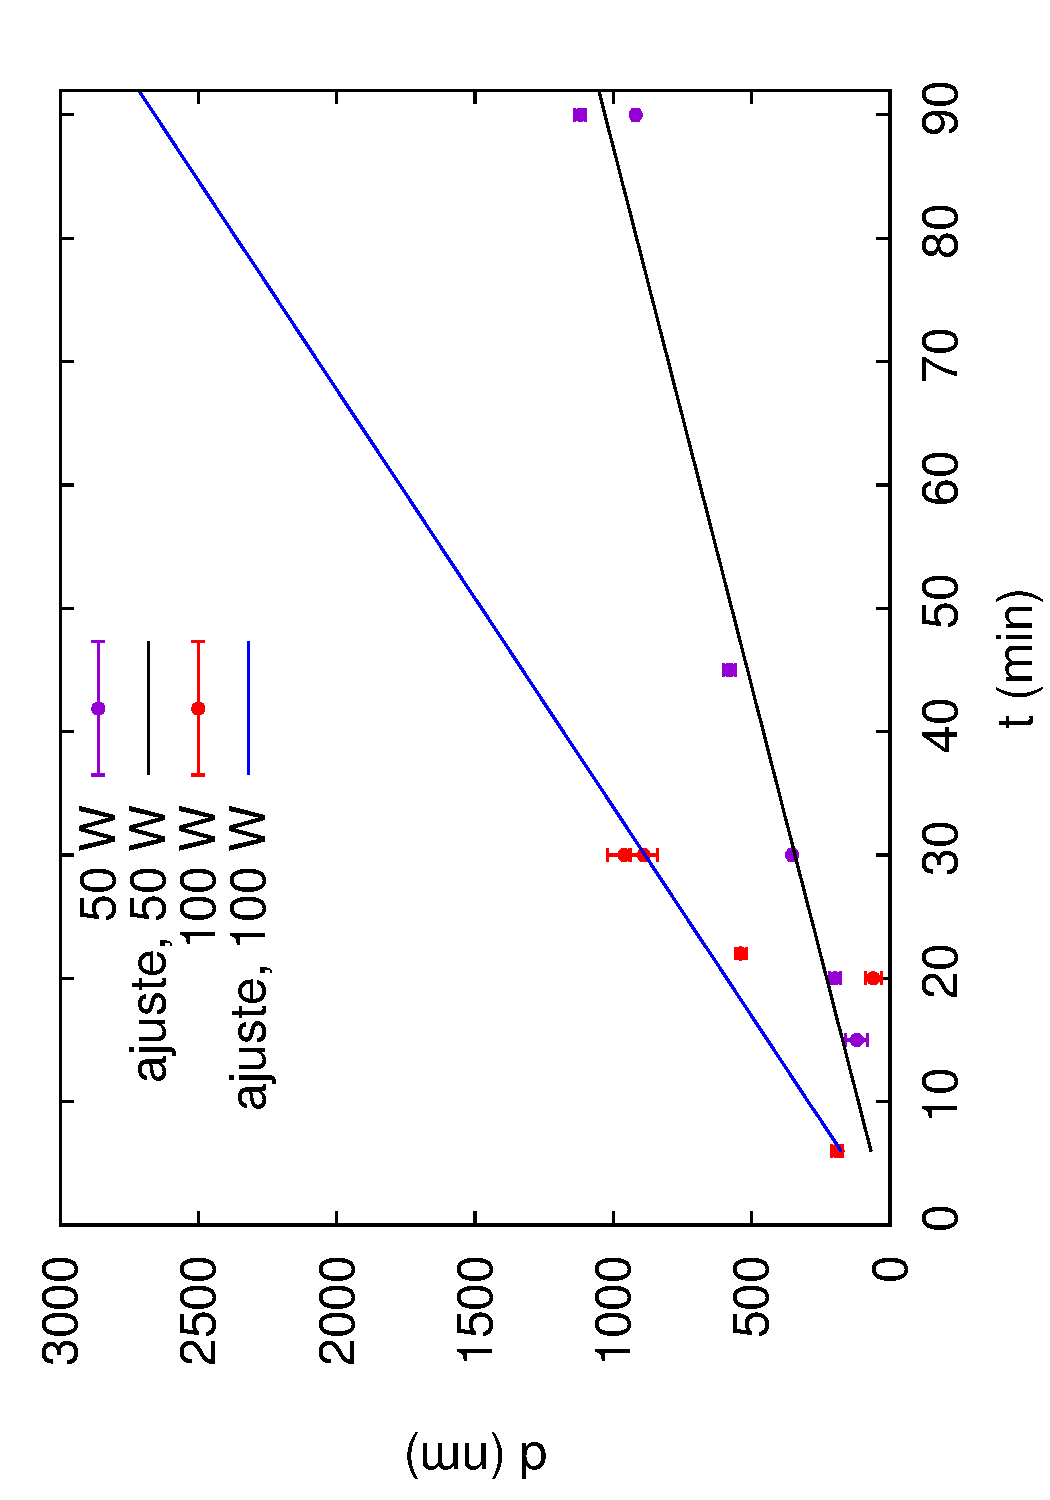
\includegraphics[width=0.5\columnwidth, angle=-90]{evst}
  \end{center}
\caption[Espesor en función del tiempo para los films de MgB$_2$ crecidos por sputtering.]{Espesor en función del tiempo para los films de MgB$_2$ crecidos. Se muestran las dos potencias utilizadas, junto con el ajuste correspondiente. Tomando como referencia dichos ajustes se estimó la velocidad de crecimiento de los films de MgB$_2$ en zafiro como $(12.9 \, \pm \, 0.5)$\,nm/s para una potencia aplicada de 50\,W y $(30 \, \pm \, 3)$\,nm/s para una potencia de 100\,W.}
\label{fig:calibracion}
\end{figure}

A partir de los resultados de los ajustes se estimó que la velocidad de crecimiento de los films de MgB$_2$ sobre zafiro, si la potencia es de 50\,W es $v_{crec, \, 50W}\, =\, (11.4 \, \pm \, 0.5)$\,nm/min, mientras que si la potencia aplicada es de 100\,W, se tiene $v_{crec,\, 100W}\, =\, (29 \, \pm \, 2)$\,nm/min. Los valores medidos se encuentran resumidos en la tabla \ref{tab:velocidadcrec}. Como puede verse, la velocidad de crecimiento a 100\,W es aproximadamente el doble de la velocidad de crecimiento a 50\,W, por lo que se puede concluir que en el régimen de presiones y potencias utilizados, la velocidad de depósito es aproximadamente lineal con la potencia aplicada, tal como se explicó anteriormente.
\begin{table}[h!]
\centering
\begin{tabular}{|c|c|c|} \hline
Potencia/W & Pendiente/(nm/min) & Ord. al origen (nm)\\ \hline
50 & $12.9\,\pm\,0.5$ & $-30\,\pm\,20$ \\ \hline
100 & $29\,\pm\,2$ & $0\,\pm\,50$ \\ \hline
\end{tabular}
\caption{Resultados de los ajustes realizados a los datos experimentales que se muestran en la Fig. \ref{fig:calibracion}.}
\label{tab:velocidadcrec}
\end{table}
\newpage
\subsection{Caracterización de la estructura cristalina por rayos X}\label{SS:rayos10}
La caracterización de muestras por medio del estudio de rayos X difractados es una de las prácticas más importantes a la hora de caracterizar materiales. La técnica consiste en incidir el material a estudiar con un haz de rayos X de longitud bien definida y medir la intensidad del haz reflejado en función del ángulo que forman la muestra y el haz incidente. Luego de una medición realizada en estas condiciones se obtiene un espectro que tiene picos a ángulos bien definidos que satisfacen la ley de Bragg:
\begin{equation}
  2 \ e \ \sin(\theta) \ = \ \lambda
  \label{eq:bragg}
\end{equation}
\noindent
siendo $\theta$ en ángulo formado entre la normal a la muestra y el detector de rayos X, $\lambda$ la longitud de onda incidente y $e$ es la separación entre la familia de planos cristalinos que cumplen la condición de Bragg. Los estudios de difracción de rayos X son muy útiles para determinar qué fases se encuentran un material y qué tipo de estructura cristalina poseen dichas fases.
\nomenclature{$e$}{Separación entre planos cristalinos.}
\nomenclature{$\theta$}{Ángulo formado entre la normal a un plano y la dirección de propagación de la radiación incidente/saliente.}

En el caso de las muestras que se desean estudiar en este trabajo aparecen dos complicaciones que vale la pena mencionar. La primera es que el bajo número atómico $Z$ del boro hace que sea muy difícil de detectar fases de boro puro en un espectro de rayos X, ya que la intensidad de los picos en un espectro de rayos X también se encuentra limitada por la sección eficaz entre el haz incidente y los átomos presentes en la muestra, que decrece como $Z^2$. El segundo factor a tener en cuenta es el siguiente: se puede ver que la integral de un pico de Bragg es proporcional al número de átomos presentes en los planos cristalinos que cumplen la condición \ref{eq:bragg}, mientras que el ancho del pico es inversamente proporcional a ese número. Esto implica que si la muestra es infinita los picos de Bragg del espectro de rayos X se aproximan a la función delta de Dirac. Sin embargo, en este trabajo se intenta caracterizar un film, por lo que, incluso si el mismo es un monocristal, es difícil que  logre satisfacer la condición de muestra infinita, con el resultado de que los picos de Bragg se vuelvan más anchos y de menor altura, si es que llegan a ser observados.

En la Fig. \ref{fig:rayos10} se muestran algunos de los espectros de difracción de rayos X para diferentes muestras, que corresponden a un barrido en la temperatura de crecimiento $T_{crec}$ de 225\,$^{\circ}$C a 275\,$^{\circ}$C (muestras BMB2S1B2 a BMB2S3B2) a 10\,mTorr y 50\,W; y una muestra en la que se incrementó la presión de Ar para el crecimiento (BMB2S6B3), mientras que la potencia fue de 50\,W y $T_{crec}\,=\,225$\,$^{\circ}$C.

Los dos picos de mayor intensidad que se encuentran señalados corresponden al sustrato de zafiro (0001) sobre el que se crecieron las muestras. Los picos más pequeños que se pueden ver antes del correspondiente a la familia de planos (0006), son debidos a la difracción de la radiación $K_{\beta}$ del Cu y a la L del W. Los picos correspondientes a la línea $K_{\beta}$ se pueden observar porque el monocromador que usa el equipo de rayos X no es perfecto, mientras que los picos debidos a la radiación de la capa L del W aparecen porque a lo largo de los años de uso del equipo, algo de W se fue depositando sobre la fuente de Cu. De esta forma, el W que se encuentra depositado es excitado junto al Cu, de modo que también emite radiación X que tiene una energía un poco diferente a la radiación X emitida por el Cu. 
\begin{figure}[tbh!]
 \begin{center}
    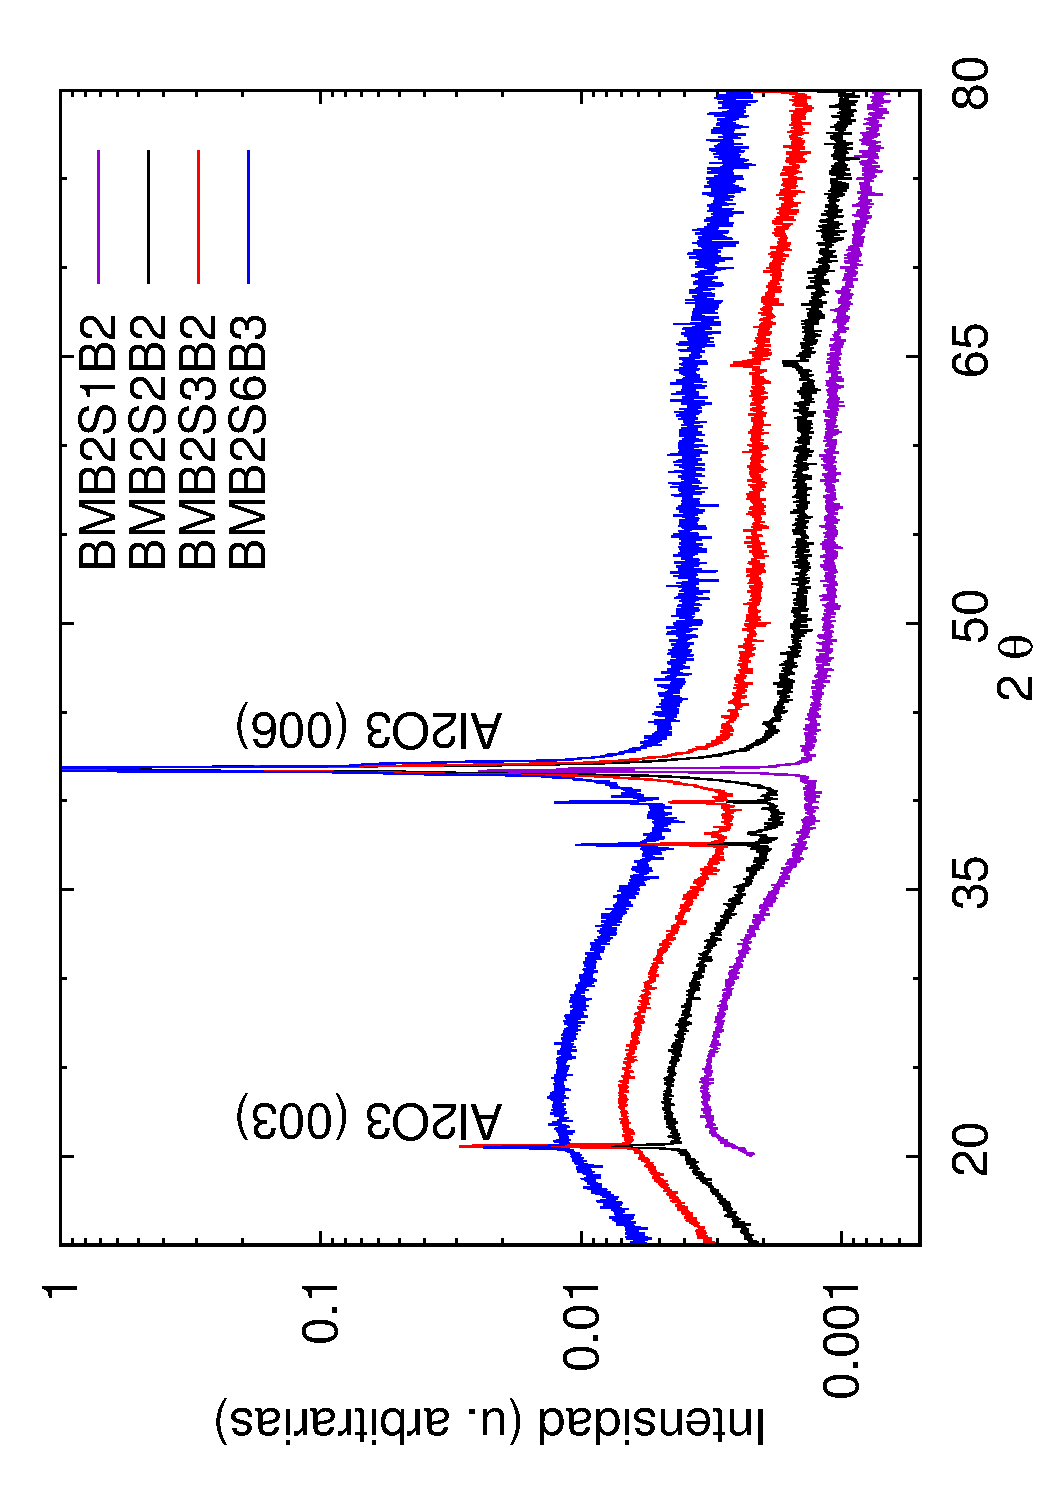
\includegraphics[width=0.5\columnwidth, angle=-90]{rayos10}
  \end{center}
  \caption[Espectro de difracción de rayos X para alguna de las muestras depositadas por sputterong.]{Espectro de difracción de rayos X para alguna de las muestras depositadas. Todos los picos observados corresponden a diferentes reflexiones del sustrato de zafiro (0001). Por otro lado puede observarse un pico muy ancho con un máximo alrededor de los 23\,$^{\circ}$. Esto se corresponde con el parámetro de red promedio del Mg policristalino.}
\label{fig:rayos10}
\end{figure}

Lo explicado en el párrafo anterior implica que todos los picos observados co\-rres\-pon\-den al sustrato de zafiro y que no se pueden apreciar picos correspondientes al MgB$_{2}$, y tampoco se pueden ver picos correspondientes a Mg o a B puros. A partir de éstos resultados pueden extraerse dos conclusiones: la primera es que se haya formado un film de MgB$_{2}$ con mala cristalinidad, o que no se haya formado la fase de MgB$_{2}$. Para verificar cuál de las dos hipótesis era la correcta, se realizaron análisis de la composición de los films y también se estudiaron las propiedades magnéticas y de transporte de los mismos. En las secciones siguientes se muestran los resultados de estos estudios.
\subsection{Caracterización de la composición por EDX}\label{SS:EDX}
La espectroscopia por rayos X característicos es una técnica ampliamente utilizada cuando se busca determinar la composición de un compuesto, y aunque no permite determinar la forma en que los elementos de un material se encuentran combinados, sí permite determinar con excelente precisión la proporción en que se encuentran dichos elementos. La técnica consiste en bombardear la muestra cuya composición se desea determinar con electrones que tienen la energía suficiente como para excitar a los electrones presentes en las primeras capas atómicas de los átomos presentes en la muestra. Posteriormente, los electrones del átomo se desexcitan emitiendo fotones que tienen una energía que es característica del átomo estudiado. A partir de colectar de estos fotones característicos se pueden construir histogramas como se muestra en la Fig. \ref{fig:SEM}, en el que se cuenta la cantidad de fotones que tienen una energía determinada, para un rango amplio de energías. El análisis de los picos observados permite identificar los elementos presentes en la muestra, así como la proporción de los mismos. Por razones parecidas a las que fueron comentadas en la sección anterior, el análisis por EDX se ve limitado para elementos livianos, siendo el B y el C  los elementos más livianos detectables por esta técnica.

En la Fig. \ref{fig:SEM} se muestran los espectros de intensidad emitida de rayos X característicos para dos de las muestras crecidas y para una pastilla de MgB$_{2}$ patrón hecha con polvo obtenido comercialmente. Dado que no se puede determinar directamente la composición de los films a partir de los métodos estándar que existen para el estudio de rayos X característicos, el método que se implementó para estimar la composición de los films fue el siguiente: del espectro obtenido para la muestra patrón, se calcula el cociente de las integrales de los picos correspondientes al B y al Mg ($Int_{B}$, $Int_{Mg}$, respectivamente). El cociente $Int_{B}/Int_{Mg}$ no tiene por qué se igual a 2. Esto es debido a que no se está haciendo la corrección de intensidades por número atómico, por absorción y por fluorescencia. Además, el hecho de que los rayos X característicos del B se encuentren en el borde de eficiencia del detector de rayos X también puede influir en que el número de cuentas que haya para los picos de B y Mg no sea proporcional a la cantidad de esos elementos en la muestra.
\begin{figure}[tbh!]
 \begin{center}
    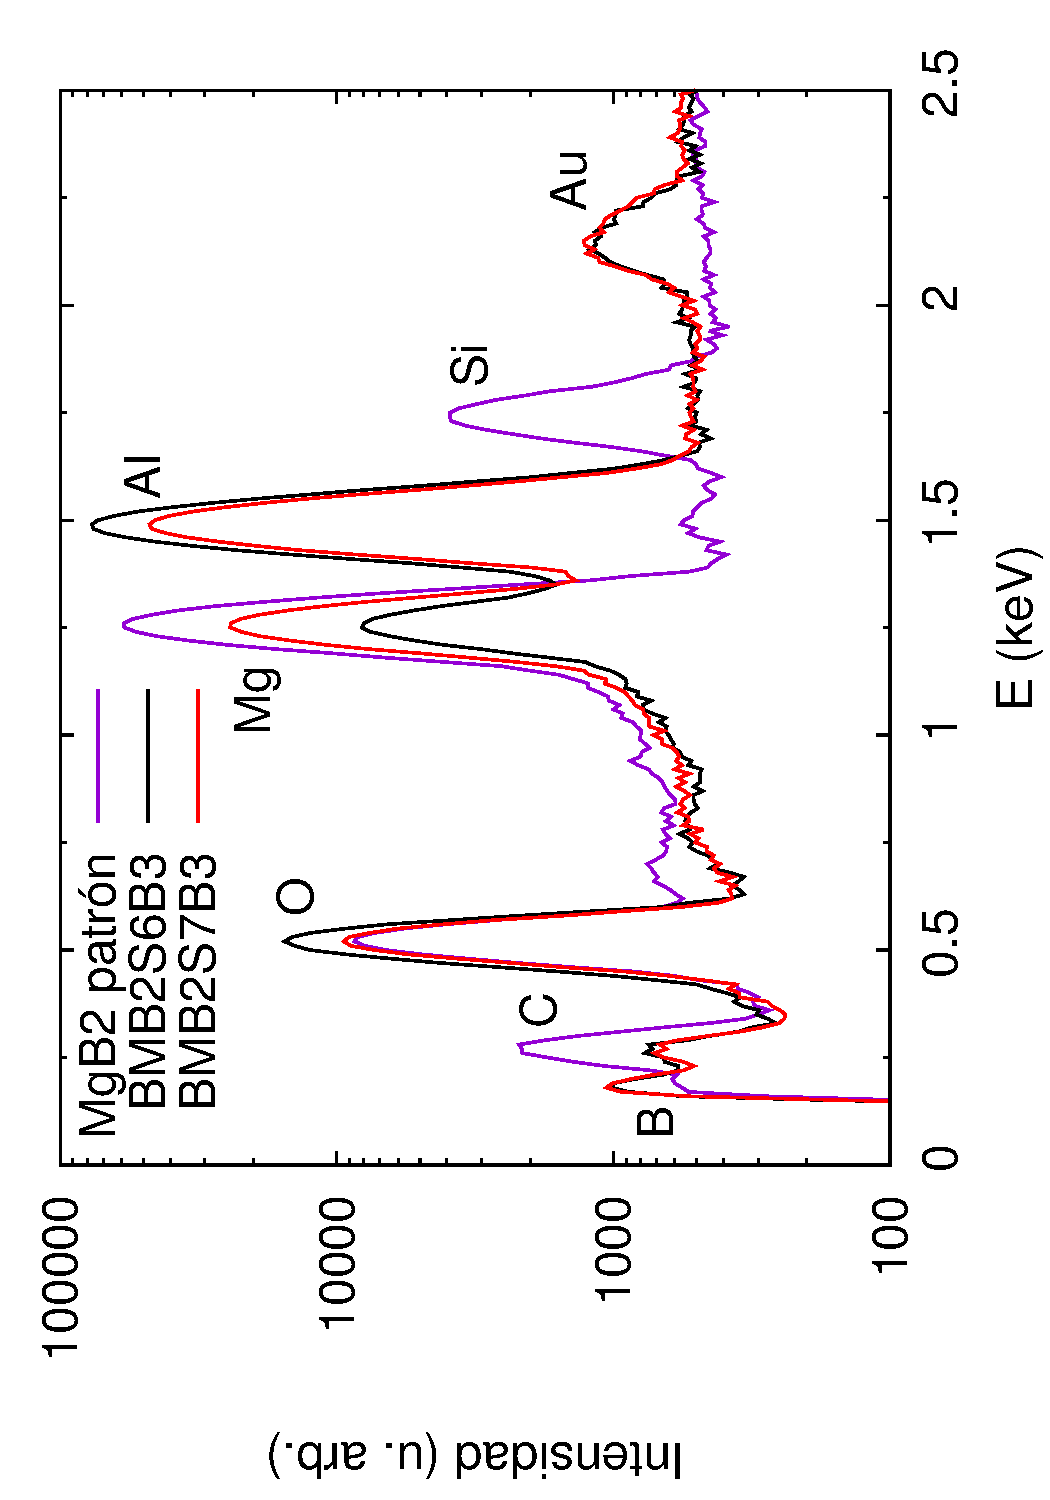
\includegraphics[width=0.55\textwidth,angle=-90]{SEM}
  \end{center}
  \caption[Espectro de la intensidad emitida de rayos X característicos para una muestra de MgB$_{2}$ patrón y para algunas de las muestras crecidas.]{Espectro de la intensidad emitida de rayos X característicos para una muestra de MgB$_{2}$ patrón y para algunas de las muestras crecidas. A partir de la comparación de las alturas relativas de los picos en el patrón se estimó la composición de los films crecidos.}
\label{fig:SEM}
\end{figure}

Una vez calculado el cociente ($Int_{B}/Int_{Mg}$)$_{bulk}$, al mismo se le asigna el valor 2, esto es, se define una constante $\varepsilon$ tal que:
\begin{equation}
  \varepsilon \ \left(\frac{Int_{B}}{Int_{Mg}}\right)_{bulk} \ = \ 2
  \label{eq:patron}
\end{equation}
%\newpage

Hecho esto, se realiza el cociente de la integral de los picos para las muestras cuya composición se desea estimar utilizando la misma constante de proporcionalidad $\varepsilon$:
\begin{equation}
  \varepsilon \ \left( \frac{Int_{B}}{Int_{Mg}} \right)_{film} \ = \ x
  \label{eq:film}
\end{equation}
\noindent
donde $x$ es la composición estimada del film. El cálculo de las áreas se hizo realizando un ajuste con una gaussiana a cada pico y luego integrando la función ajustada, sustrayendo una línea base que era una parábola. En los casos en que el pico de interés se superponía con el de otro elemento (por ejemplo, el B y el C, o el Mg y el Al) la línea de base consistió además en una gaussiana del pico vecino. Los centros de las gaussianas se mantenían fijos y eran tomados a partir de los datos de las líneas de emisión de cada elemento. En la Fig. \ref{fig:fiteos} se muestra un ejemplo del resultado de esta operación para uno de los films estudiados.
 \begin{figure}[tbh!]
   \begin{center}
	 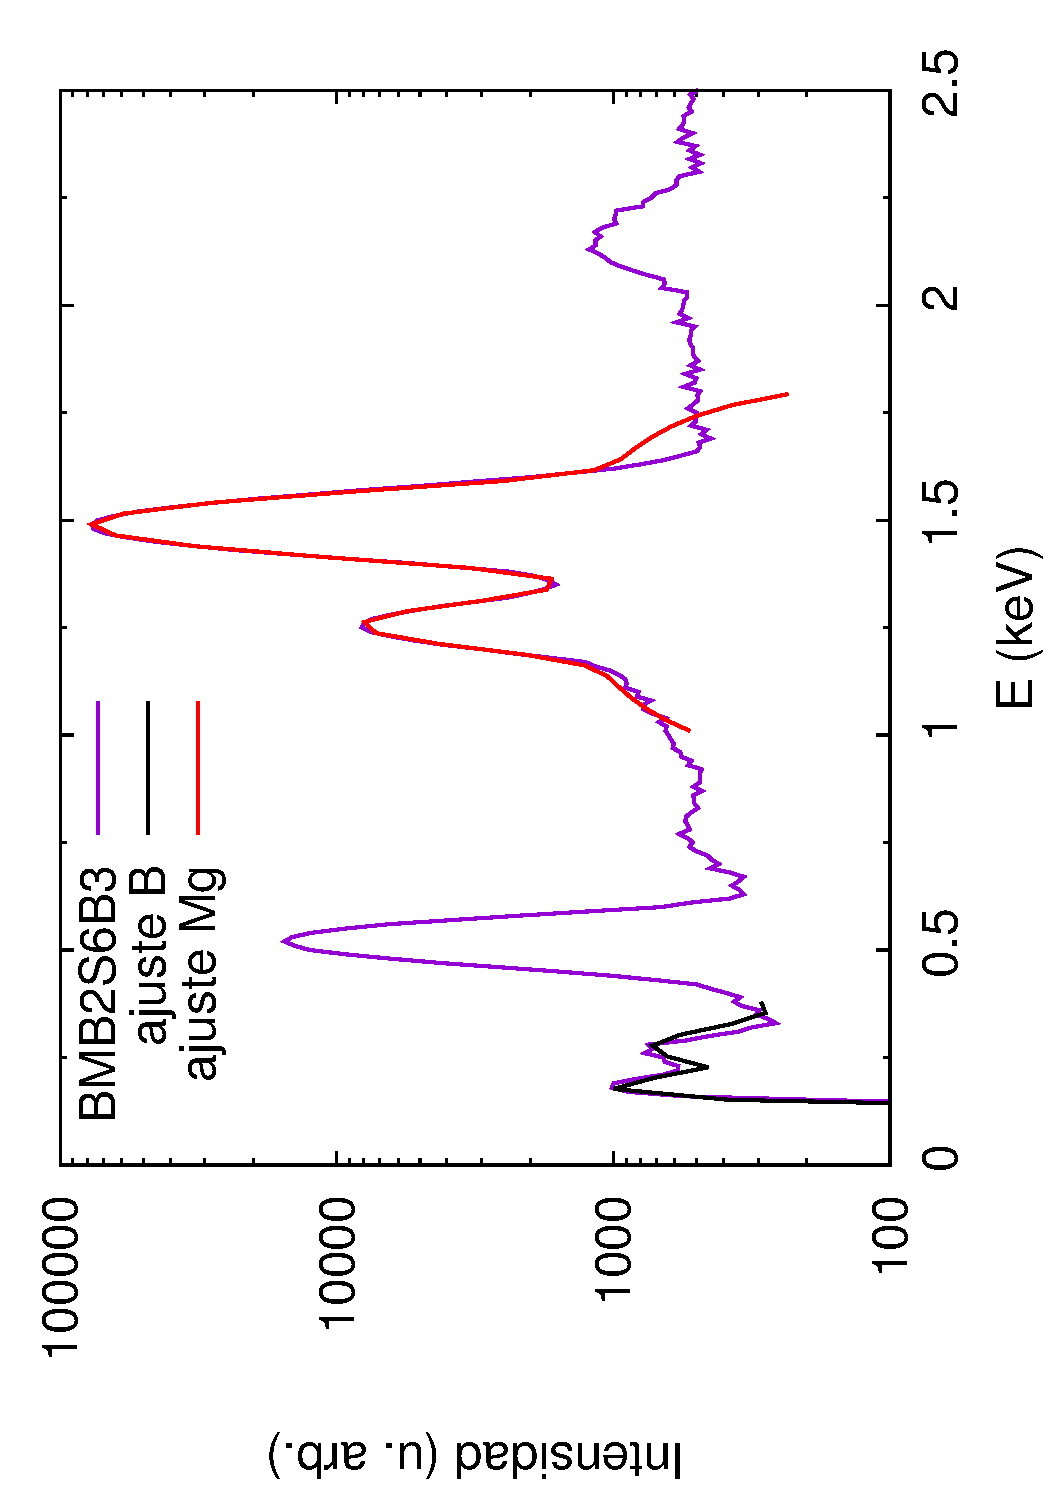
\includegraphics[width=0.55\textwidth, angle=-90]{fiteo}
   \end{center}
   \caption[Ejemplo del procedimiento empleado para estimar la composición de los films.]{Ejemplo del procedimiento empleado para estimar la composición de los films. Se ajustó una gaussiana al pico cuya área se deseaba estimar. Además se sumó una línea de base que consisitió en una parábola más una gaussiana asociada al pico vecino. Una vez sustraída la línea de base se calculó la integral de la gaussiana ajustada. A partir de la comparación de los cocientes de las integrales de los picos de B y Mg de los films con el patrón se estimó la composición de las muestras crecidas.}
   \label{fig:fiteos}
 \end{figure}

 A partir de los ajustes y cálculos realizados se estimó que la constante de proporcionalidad tiene el valor $\varepsilon\,=\,300\,\pm\,50$. Con $\varepsilon$ así calculado se construyó la tabla \ref{tab:composicionSEM}, en la que se compara la proporción B/Mg para las diferentes muestras estudiadas, junto con los parámetros de crecimiento relevantes que fueron modificados.

En las las tablas \ref{tab:depositos} y \ref{tab:composicionSEM} puede verse que la muestra BMB2S6B3 fue crecida en las mismas condiciones que la muestra BMB2S7B3, excepto que en la segunda la potencia aplicada al blanco era de 100\,W en vez de 50\,W. A partir de esto se puede suponer que un incremento en la potencia aplicada mejora la proporción B/Mg del film. Esto puede deberse a dos razones: la primera es que incrementar la velocidad de depósito implique de alguna forma un incremento en la presión de Mg en la proximidad del film, lo que produciría que deposite más Mg y por ende que aumente la proporción del mismo. La otra es que al incrementar la velocidad de depósito, es posible que el Mg quede ``atrapado'' por las demás partículas que están llegando del blanco y no tenga tiempo de evaporarse nuevamente.
 \begin{table}[h!]
  \centering
  \begin{tabular}{|c|c|c|c|}\hline
	Muestra	& Potencia/W & p/mTorr & Proporción B/Mg\ \\ \hline
	Patrón & - & - & 2 \\
	BMB2S6B3 & 50 & 100 & 27 $\pm$ 5 \\
	BMB2S7B3 & 100 & 100 & 8 $\pm$ 2 \\ 
	BMB2S1B4 & 100 & 50 & 28 $\pm$ 10 \\
	BMB2S3B3 & 100 & 10 & 14 $\pm$ 2 \\ \hline
  \end{tabular}
  \caption[Proporción B/Mg para las muestras estudiadas por EDX.]{Proporción B/Mg para las muestras estudiadas por EDX. Se muestran además los parámetros de crecimiento que cambiaron entre las diferentes muestras. En todos los casos la temperatura de crecimiento era 225\,$^{\circ}$C y la altura de crecimiento era 2,75, de acuerdo a lo indicado en la sección \ref{S:sputproc}. La única diferencia entre BMB2S6B3 Y BMB2S7B3 es que la primera fue crecida con una potencia aplicada de 50\,W mientras que la segunda lo fue con 100\,W. Las últimas tres muestras fueron crecidas con una potencia de 100\,W, pero con presión de Ar de 100\,mTorr, 50\,mTorr, 10\,mTorr, respectivamente.}
  \label{tab:composicionSEM}
\end{table}
%\newpage 
\nomenclature{$Int_{E}$}{Integral del pico correspondiente al elemento $E$, en un espectro de EDX.}
%\begin{figure}[tbh!]
%  \begin{center}
% 	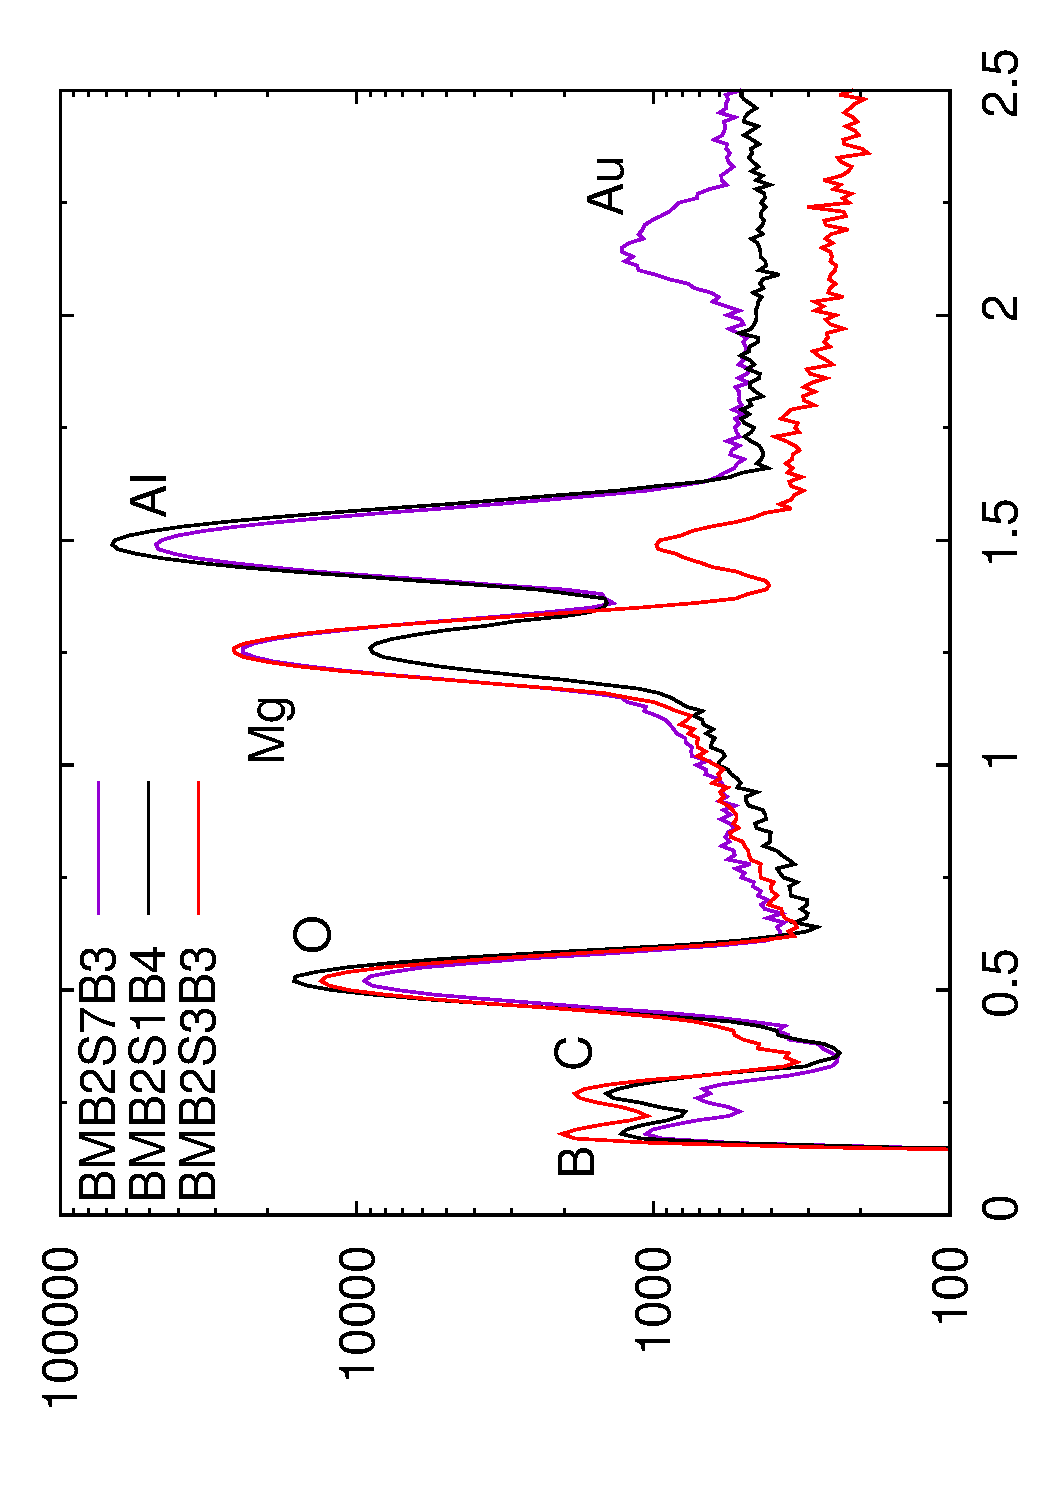
\includegraphics[width=0.55\textwidth, angle=-90]{SEM_cascada}
%  \end{center}
%  \caption{}
%  \label{fig:SEMcascada}
%\end{figure}

También se estudió el efecto que tiene la presión de Ar en la cámara en la composición final. En la tabla \ref{tab:composicionSEM} se muestra la proporción B/Mg de tres muestras crecidas en las mismas condiciones de temperatura y potencia, pero con diferente presión. Como se explicó al principio del capítulo, la presión de Ar en la cámara regula el camino libre medio de las partículas que salen del blanco, es decir, la cantidad de colisiones que sufren estas partículas antes de llegar al sustrato. De esta forma se puede controlar la energía cinética que tienen las mismas al momento de depositarse en el sustrato, lo que influye en la topografía del film, su adherencia con el sustrato y la estructura cristalina que se pueda formar.
 \begin{figure}[tbh!]
   \begin{center}
	 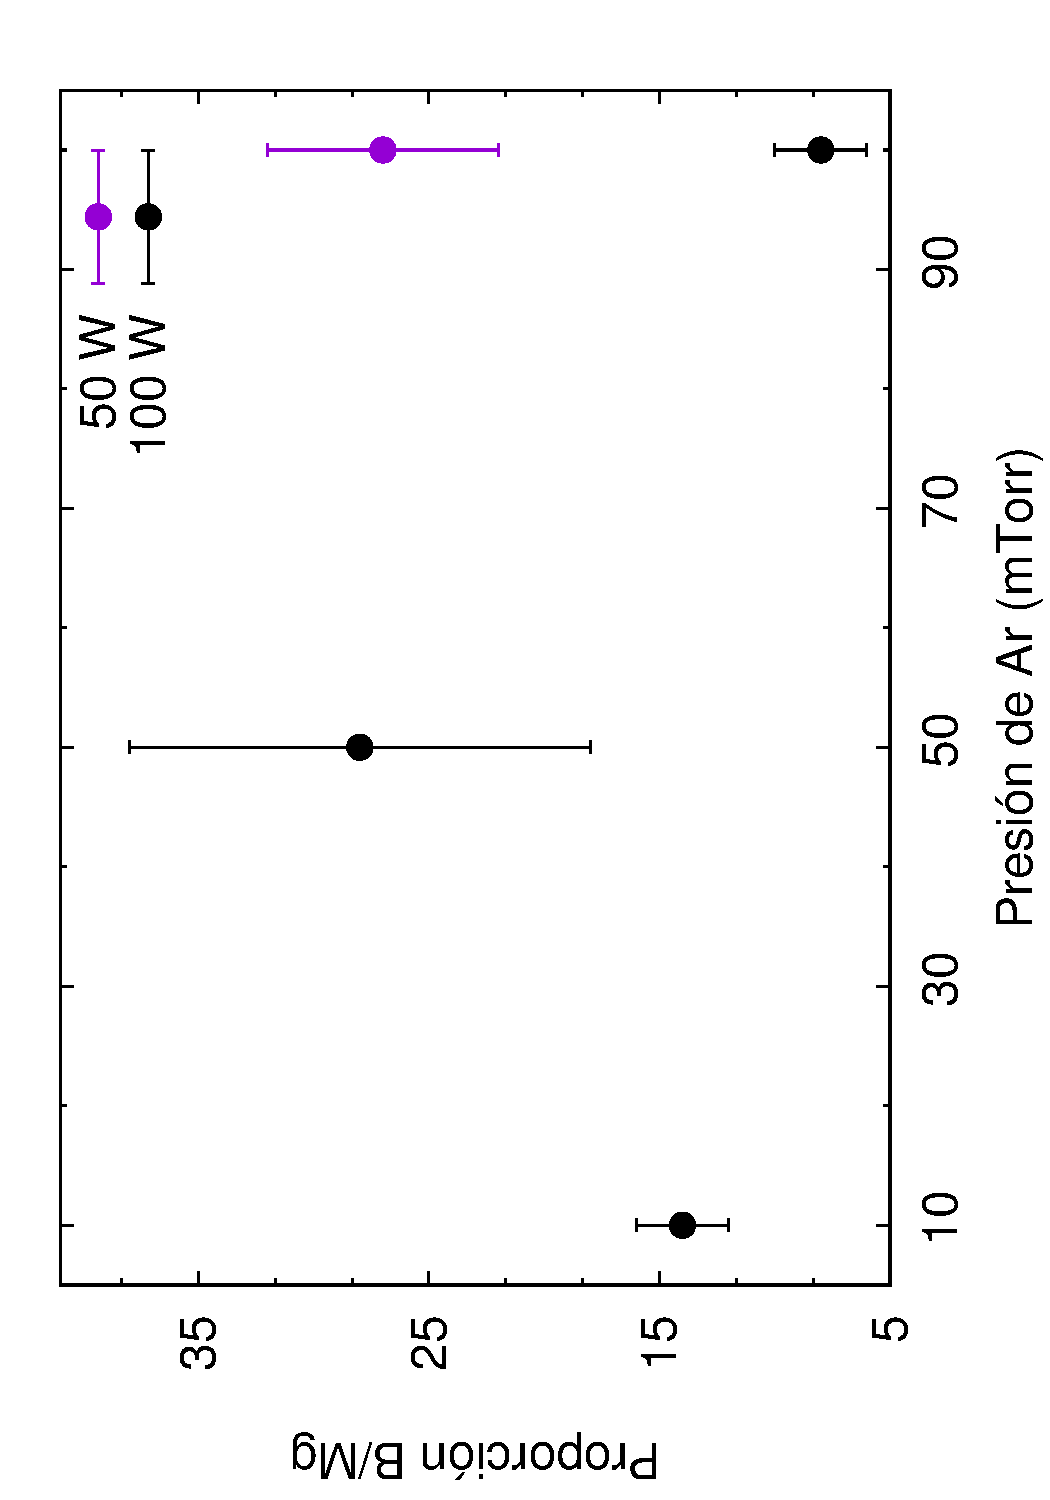
\includegraphics[width=0.55\textwidth, angle=-90]{xvsp}
   \end{center}
   \caption[Proporción B/Mg para films crecidos con diferente presión de Ar en la cámara de sputtering.]{Proporción B/Mg para films crecidos con diferente presión de Ar en la cámara de sputtering. También se muestra una medición en la que el parámetro variado fue la potencia aplicada al blanco. Puede verse que mientras que la potencia tiene un claro efecto positivo en la composición del film, el efecto de la presión no es del todo claro.}
   \label{fig:xvsp}
 \end{figure}
\newpage

 Al analizar el comportamiento de la proporción B/Mg con la potencia puede apreciarse que disminuye claramente al aumentar la potencia que se aplica al blanco, es decir, al aumentar la velocidad de crecimiento. En el gráfico se muestran barras de error que corresponden a una desviación de 1 $\sigma$, pero los valores se encuentran separados incluso si se considera una desviación de 2 $\sigma$, lo que valida la conclusión de que al incrementarse la velocidad de crecimiento, la proporción B/Mg se aproxima a la correcta. A partir de esto se podría plantear la propuesta de incrementar más aún la potencia aplicada al blanco, en busca de lograr la proporción B/Mg deseada. Sin embargo, esto no es posible ya que una potencia mayor podría llevar a romper el blanco. A partir de este inconveniente fue que se planteó estudiar el efecto que tiene la presión de Ar en la proporción B/Mg, resultando que ambas variables están relacionadas en forma no monótona. Esto es lo que podría interpretarse si se considera una desviación
%\newpage
\noindent
 de 1 $\sigma$ en la Fig. \ref{fig:xvsp}, pero si se considera la desviación de 2 $\sigma$ alrededor de los valores observados, la conclusión es que no existe una dependencia clara entre la proporción B/Mg y la presión de Ar en la cámara.
\subsection{Caracterización de la composición por RBS}\label{SS:RBS}
El estudio de la composición por RBS consiste en bombardear el film con iones que tienen una energía conocida y estudiar el espectro de energía con que salen las partículas después de la colisión con la muestra. Como proyectil de prueba se suelen utilizar iones de H o de He, en función de la masa de los átomos presentes en la muestra. Como los iones que están presentes en la muestra son livianos, el espectro de energía producido resulta ser bastante sensible si los elementos presentes en la muestra tienen $Z$ pequeño, ya que en ese caso la transferencia de energía es máxima. En este sentido la espectroscopia por RBS puede considerarse la contraparte de la técnica EDX. La composición del material puede estimarse proponiendo un modelo de capas del material y realizando un ajuste en el que los parámetros libres son el espesor y la composición de cada capa.

 \begin{figure}[tbh!]
   \begin{center}
	 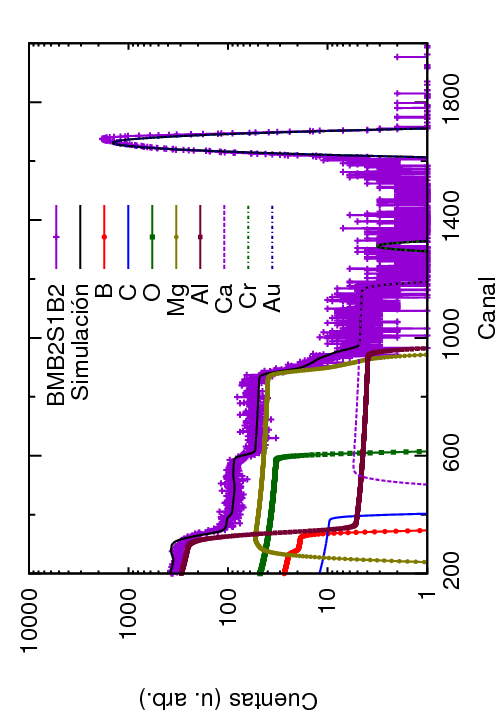
\includegraphics[width=0.58\textwidth, angle=-90]{RBS}
   \end{center}
   \caption[Espectro RBS típico observado para las muestras estudiadas.]{Espectro RBS típico observado para las muestras estudiadas. El espectro que se observa corresponde a la muestra BMB2S1B2. La presencia de Au y Cr se puede explicar teniendo en cuenta que sobre la muestra se evaporaron contactos para medir propiedades de transporte, y el Al y O corresponden al sustrato de zafiro.}
   \label{fig:RBS}
 \end{figure}

 En la Fig. \ref{fig:RBS} se muestra el espectro RBS típico que se pudo observar en las muestras estudiadas. Como puede verse, el método permite observar el Mg y el B presente en la muestra, así como el Al y el O presentes en el sustrato de zafiro (fórmula química Al$_2$O$_{3}$). También se observan impurezas de C y Ca y rastros de Au y Cr debidos a contactos que se evaporaron sobre la muestra para medir propiedades de transporte. En la tabla \ref{tab:composicionRBS} se encuentran resumidos los resultados obtenidos del cálculo de la composición B/Mg para las diferentes muestras estudiadas por medio de la téc\-ni\-ca RBS.

 \begin{table}[h!]
  \centering
  \begin{tabular}{|c|c|c|c|}\hline
	Muestra	& Potencia/W & p/mTorr & Proporción B/Mg\ \\ \hline
	BMB2S1B2 & 50 & 10 & 3,62 \\
	BMB2S3B3 & 100 & 10 & 4,49 \\
	BMB2S4B3 & 50 & 50 &  2,38 \\ \hline
  \end{tabular}
  \caption[Proporción B/Mg para las muestras estudiadas por medio de la técnica RBS.]{Proporción B/Mg para las muestras estudiadas por medio de la técnica RBS. Se muestran además los parámetros de crecimiento que cambiaron entre las diferentes muestras. En todos los casos la temperatura de crecimiento era 225\,$^{\circ}$C y la distancia era 2,75. Las mediciones y el análisis de los datos fueron realizados por los Dres. S. Suárez y L. M. Rodriguez.}
  \label{tab:composicionRBS}
\end{table}

Si se comparan las tablas \ref{tab:depositos} y \ref{tab:composicionRBS} el primer punto llamativo es que se tiene una misma muestra (la BMB2S3B3) que presenta diferentes composiciones para cada técnica, incluso más allá del error de ambos métodos, lo que no es del todo sorprendente si se tienen en cuenta las diferencias que existen entre los métodos utilizados para hacer la estimación. En el caso de la técnica EDX cabe tener en cuenta que se intentó estimar la composición del B, un elemento que se encuentra en el límite de confianza de la técnica, por lo que las conclusiones que se pueden sacar del análisis EDX son más bien cualitativas que cuantitativas. En el caso del estudio por RBS, aunque es una técnica con más sensibilidad al B que el EDX, cabe mencionar que, como se observa en la Fig. \ref{fig:RBS}, el espectro que se espera del boro ocurre a bajas energías, donde la resolución del detector utilizado para hacer el estudio RBS es más pobre.
\newpage
Teniendo en cuenta las imprecisiones observadas en los métodos utilizados para determinar la estequiometría y estructura cristalina de los films crecidos, se decidió completar la caracterización de los films crecidos con mediciones de magnetización y transporte. Este tipo de mediciones, que se encuentran detalladas en la sección siguiente, permitió obtener una descripción completa de las propiedades de los films crecidos.
\subsection{Caracterización de las propiedades magnéticas y de transporte}\label{SS:sptucarac}
Como se explicó al principio del capítulo, la estequiometría de un film y la estructura cristalina formada en el mismo son dos cosas diferentes. Es decir, es posible que se hayan formado granos de MgB$_2$ desconectados entre si, y que en el resto del material exista un exceso de B, lo que explicaría la estequiometría observada, y aún así daría una señal en el SQUID. También es posible que se haya formado un camino de MgB$_2$ con un área muy pequeña, lo que daría una señal imperceptible en el SQUID pero sería observable en una medición de transporte. De ahí que mediciones de magnetización en conjunto con mediciones de transporte permiten determinar completamente si se ha podido formar el superconductor MgB$_2$ en alguno de los films crecidos.
 \begin{figure}[tbh!]
   \begin{center}
	 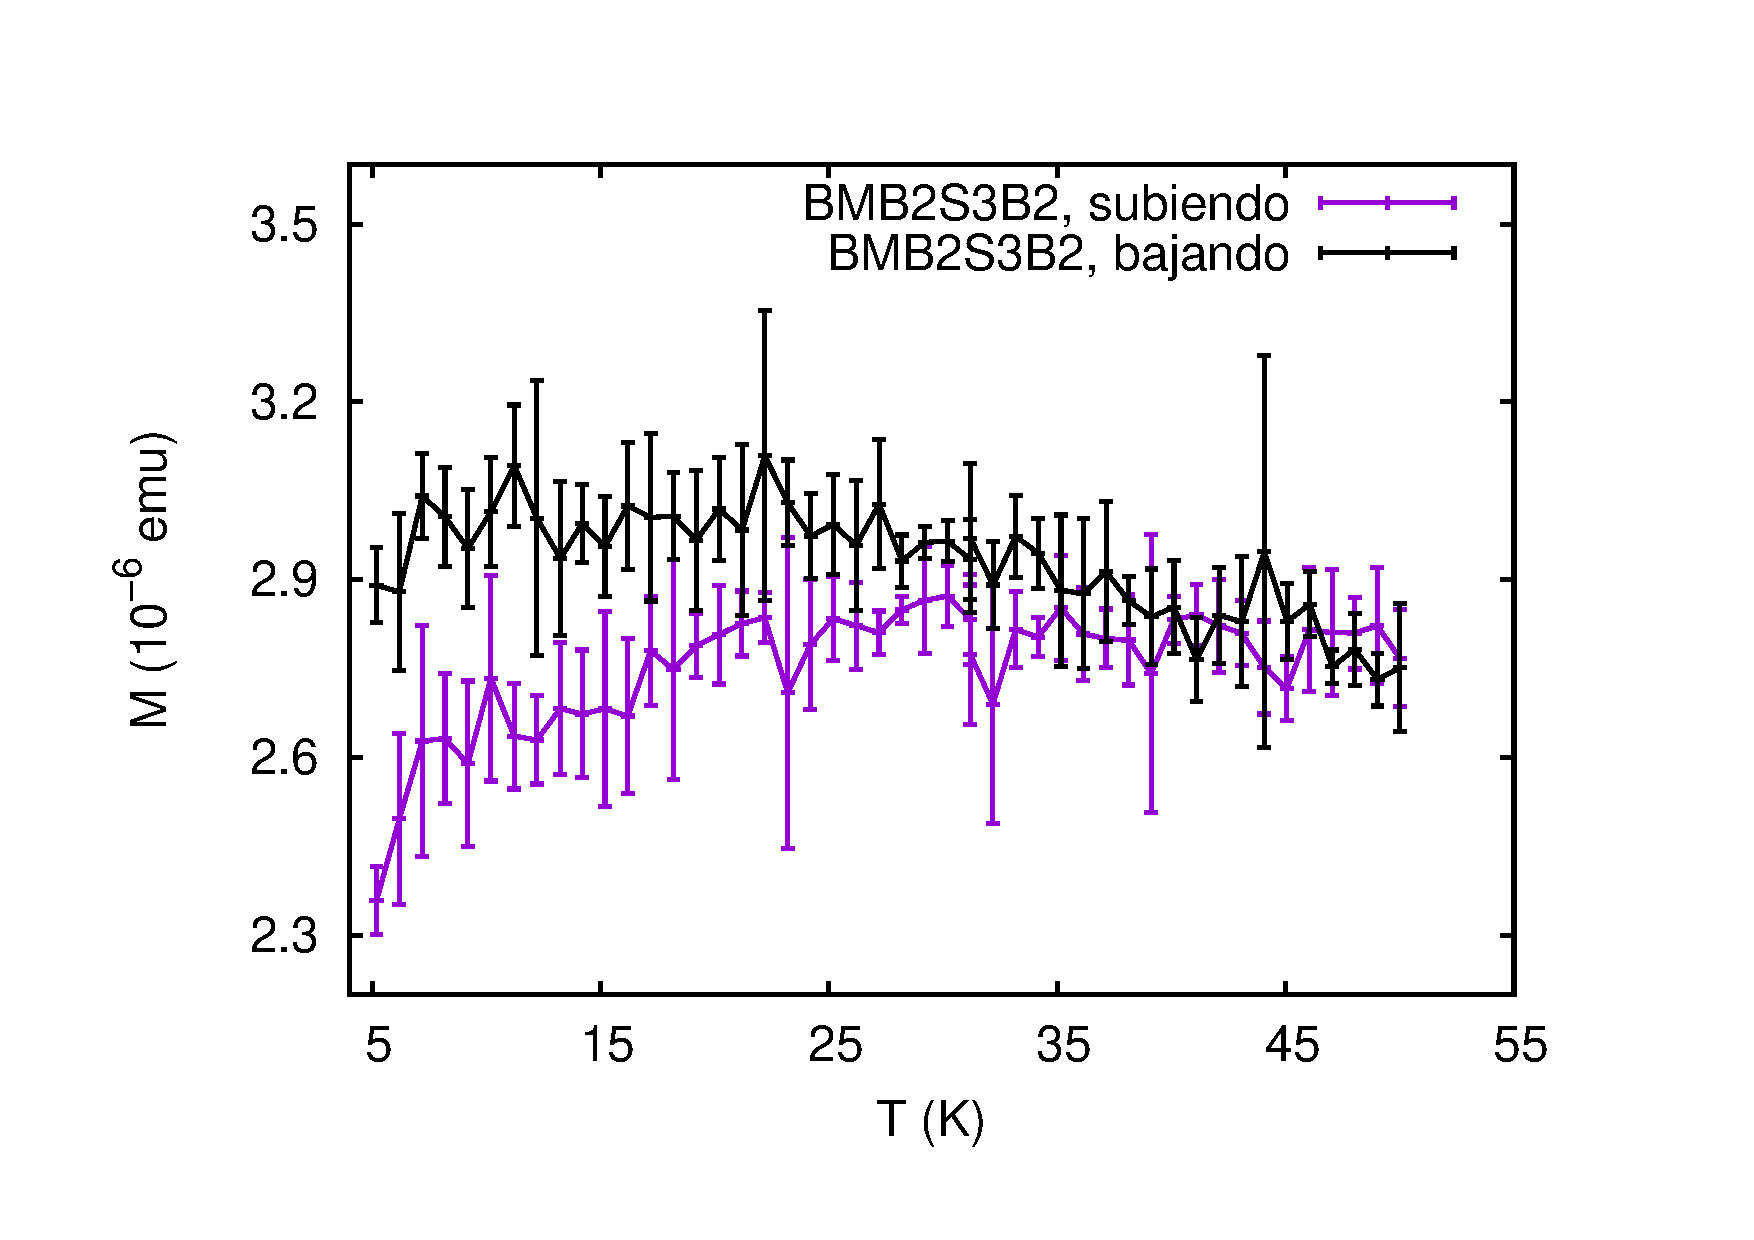
\includegraphics[width=0.9\textwidth, angle=0]{BMB2S4B2_MvsT}
   \end{center}
   \caption[Magnetización en función de la temperatura para la muestra BMB2S3B2, después de realizar un recocido con una pastilla de Mg puro.]{Magnetización en función de la temperatura para la muestra BMB2S3B2, después de realizar un recocido con una pastilla de Mg puro. La aparente irreversibilidad observada se encuentra dentro de límite de resolución del instrumento y no es una prueba confiable de la existencia de superconductividad. A partir de esto se concluyó que los films crecidos por sputtering no resultaron ser superconductores, ni siquiera luego del proceso de recocido. El fallo del recocido se debió probablemente a que el mismo ocurrió a una temperatura demasiado baja.}
   \label{fig:mvst}
 \end{figure}
\newpage
 Dentro de los films depositados por sputtering pudo distinguirse que, al incrementarse la presión de Ar en la cámara durante el crecimiento, los mismos pasaban de ser trans\-pa\-ren\-tes a ser de un color marrón claro. Los primeros eran completamente aislantes mientras que los segundos tenían una resistencia del orden de los k$\Omega$, que es el orden de magnitud de resistencia esperable para un film. Sin embargo, ninguno mostró algún tipo de señal en el SQUID o en mediciones de transporte, probablemente debido a la falta de Mg en los films. Teniendo en cuenta esto se decidió recocer los films crecidos por sputtering junto con una pastilla de Mg puro (pureza 99,5 \%), con el fin de compensar el exceso de boro en las muestras. Se decidió intentar con Mg, y no con MgB$_2$, para reducir la temperatura del recocido. Esto se podía lograr con Mg ya que el mismo tiene un punto de fusión menor que el MgB$_2$, y lo que permite lograr una mayor presión parcial de Mg a una temperatura inferior. Como no existen fases estables de Mg-B  con exceso de Mg, el único compuesto que se debería formar en un proceso de este estilo es el MgB$_2$. Teniendo en cuenta esto se realizaron recocidos de alrededor de 20 hs. de los films crecidos con Mg siguiendo el mismo procedimiento que el utilizado en el capítulo \ref{C:evap}, bajando la temperatura de recocido a 630\,$^{\circ}$C.
 \begin{figure}[tbh!]
   \begin{center}
	 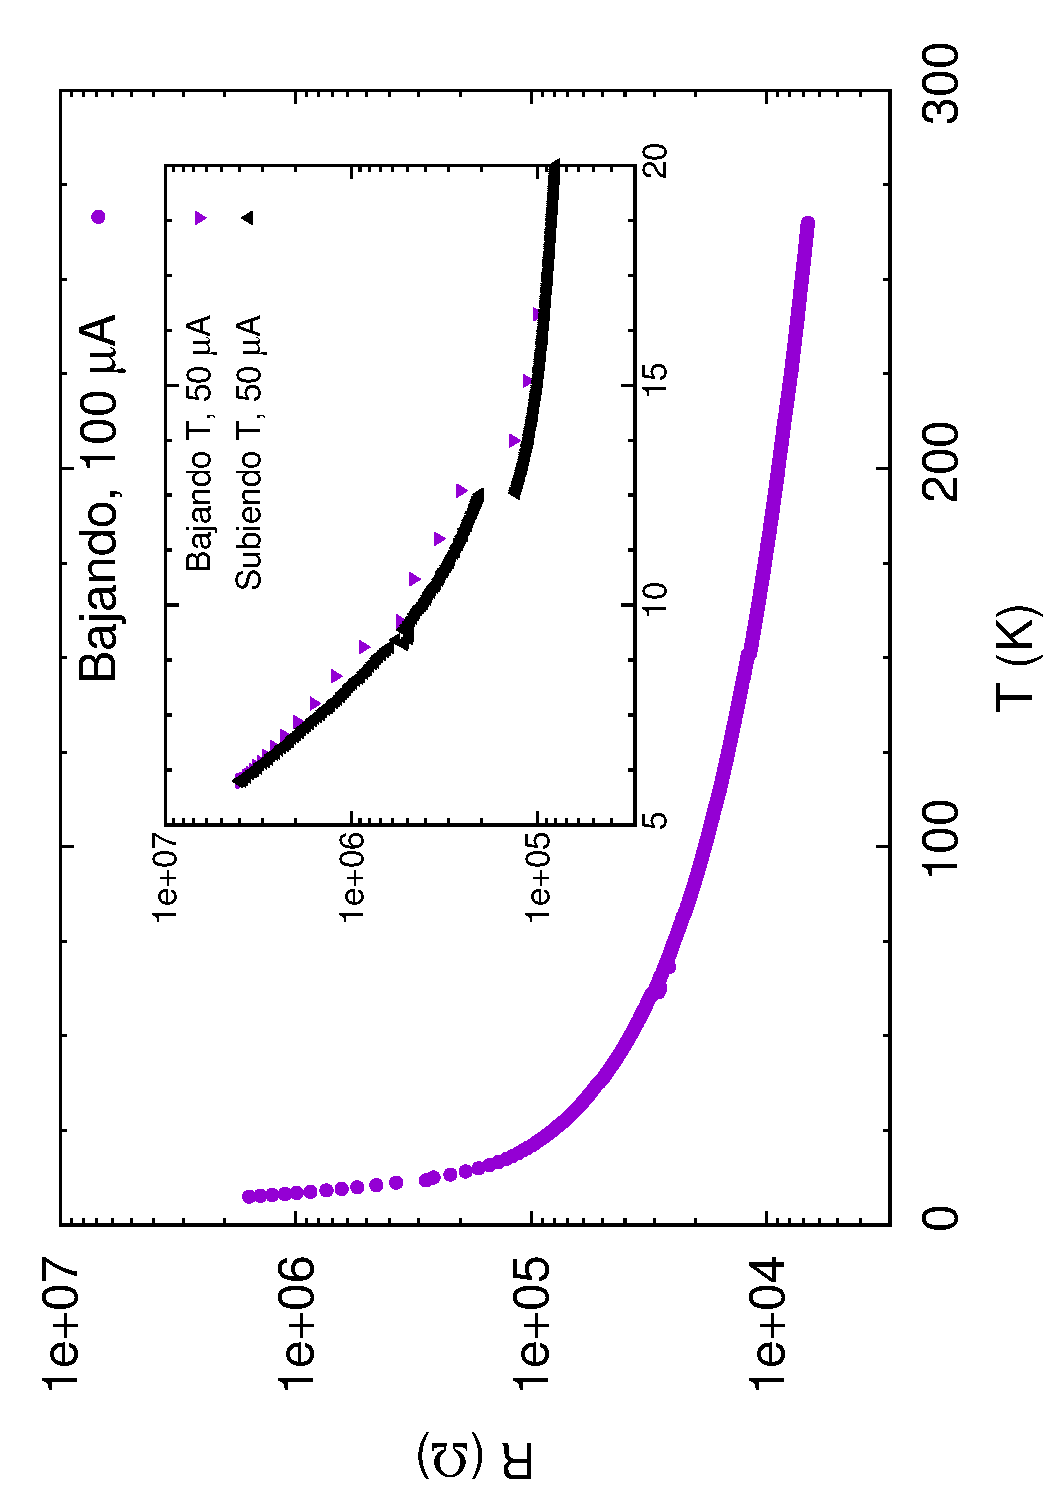
\includegraphics[width=0.55\textwidth, angle=-90]{Rvst_BMB2S1B1}
   \end{center}
   \caption[Medición de la resistencia en función de la temperatura para la muestra BMB2S1B1, luego de ser recocida.]{Medición de la resistencia en función de la temperatura para la muestra BMB2S1B1, luego de ser recocida. El recocido llevó a que las muestras pasasen de ser transparentes y aislantes a tener un color negruzco y una resistencia de algunos k$\Omega$. Puede observarse, sin embargo que la muestra tiene un comportamiento semiconductor en vez de metálico, que es lo que se esperaría si el film fuera de MgB$_2$. A parir de esto se elaboró la conclusión que las películas delgadas no incorporaron la cantidad suficiente de Mg durante el recocido. El salto en resistividad observado a alrededor de 12\,K se debe a un problema con los contactos.}
   \label{fig:rvstS1B1}
 \end{figure}
 
 Luego de extraer a las muestras del recocido se notó que las muestras que eran transparentes adquirieron un color negruzco y pasaron de ser completamente aislantes a tener una resistencia de algunos k$\Omega$. Las muestras que eran marrones se volvieron algo más oscuras pero aparte de eso no mostraron cambios perceptibles en sus propiedades. Se volvió a medir la magnetización en las muestras recocidas, sin embargo, los resultados de las mediciones de magnetización, que se ven la Fig. \ref{fig:mvst}, dieron los mismos resultados que con las muestras antes del recocido. Si bien puede observarse cierta irreversibilidad en la magnetización, el valor de la misma se encuentra cerca del límite de resolución del instrumento. Como se dijo previamente, este comportamiento se observó sistemáticamente en todos los films crecidos, antes y después del recocido.

%\subsection{Caracterización de las propiedades de transporte}\label{SS:Rvst}
%\newpage
 También se procedió a caracterizar las propiedades de transporte de los films recocidos, mostrándose en la Fig. \ref{fig:rvstS1B1} los resultados obtenidos para la muestra BMB2S1B1, donde se puede apreciar que el comportamiento de la resistencia del film al disminuir la temperatura se asemeja más al de un semiconductor que al del MgB$_2$. El salto observado a $T \ \approx \  12$\,K es debido a problemas con los contactos colocados sobre la muestra. La conclusión que puede extraerse tanto de las mediciones de magnetización como de las de transporte es que no se ha podido lograr la fase MgB$_2$, ni siquiera luego del proceso de recocido. El motivo por el que el recocido haya fallado se debe probablemente a que como la temperatura a la que ocurrió el mismo no fue lo suficientemente alta, no se pudo hacer difundir la cantidad suficiente de Mg a través del film como para formar la fase MgB$_2$. A partir de esto resulta claro que si se busca fabricar los films por medio de un proceso de recocido resulta necesario realizarlo utilizando MgB$_2$. De esta forma se puede incrementar la temperatura a la que ocurre el recocido de modo de permitir a los átomos de Mg difundir a través del film. Esta solución trae aparejado el problema de que al aumentar la temperatura, el sustrato va a reaccionar con la muestra depositada en él, por lo que si desea continuar con el proceso de recocido, es preciso buscar un sustrato que reaccione poco o nada con el MgB$_2$ a altas temperaturas.
%\begin{figure}[tbh!]
%  \begin{center}
%	 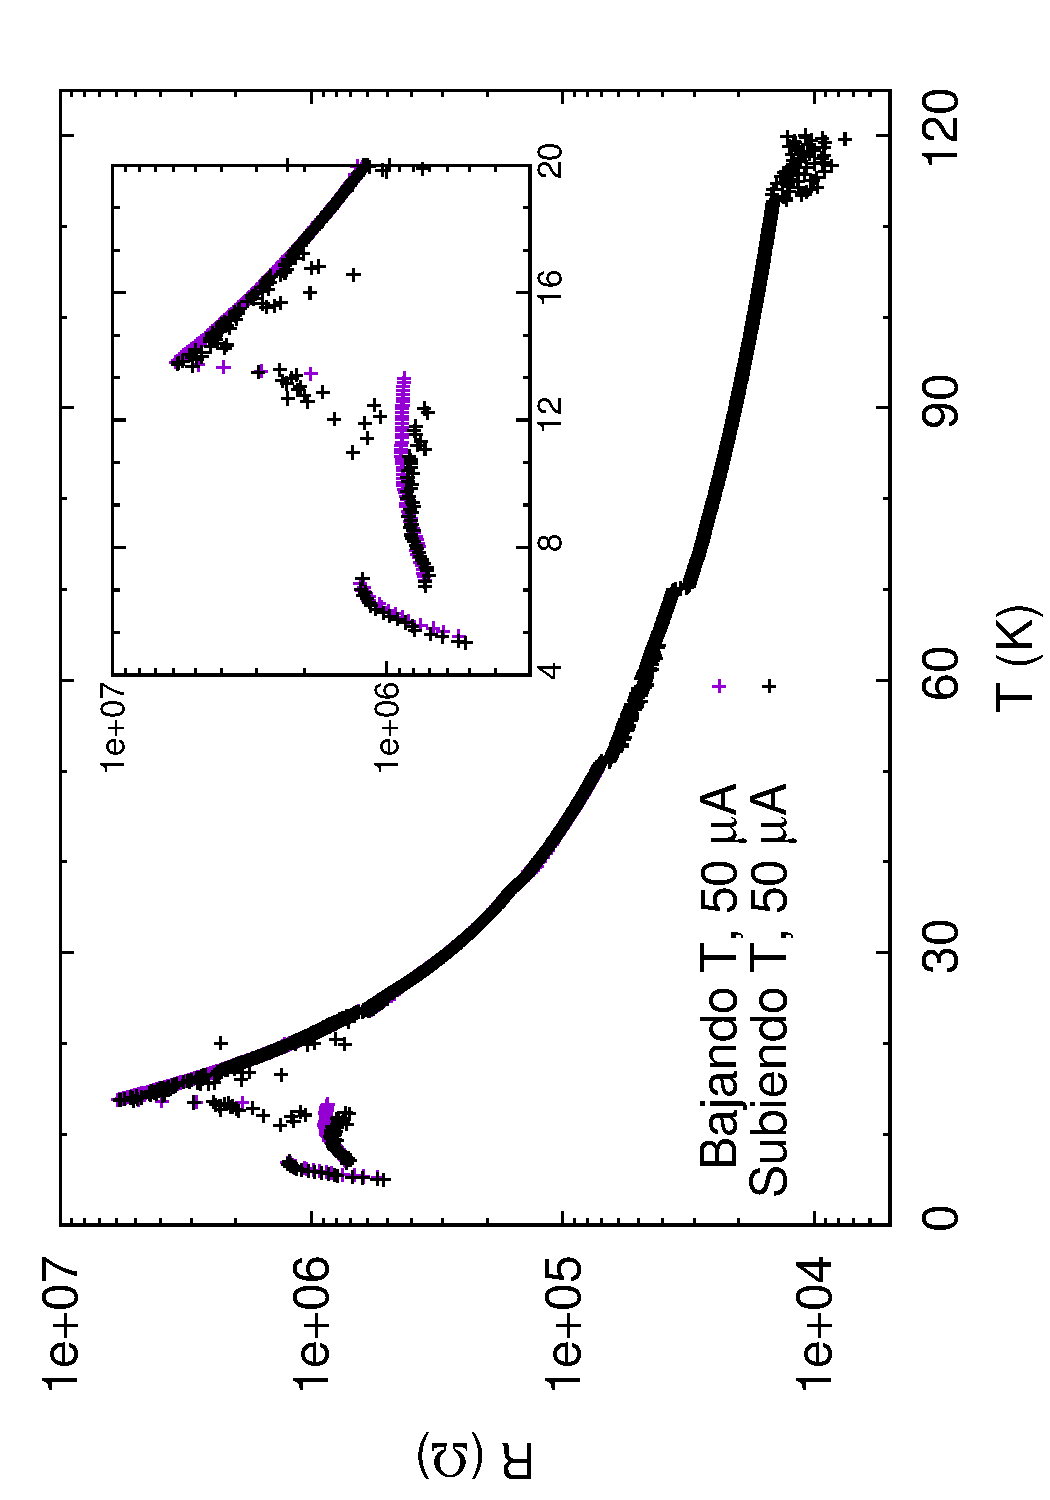
\includegraphics[width=0.55\textwidth, angle=-90]{Rvst_BMB2S2B1}
 %  \end{center}
 %  \caption{Rvst para BMB2S2B1}
 %  \label{fig:rvstS2B1}
 %\end{figure}
\nomenclature{$T_{crec}$}{Temperatura a la que se crece un film.}
\nomenclature{$v_{crec}$}{Velocidad de crecimiento de un film.}
\nomenclature{EDX}{Siglas en inglés para espectroscopia por rayos X característicos.}
\nomenclature{RBS}{Siglas en inglés para retrodispersión de Rutherford.}
\nomenclature{$\varepsilon$}{Constante de proporcionalidad.}
\nomenclature{$x$}{Proporción B/Mg de una muestra.}
\section{Análisis del método}\label{S:sputanalisis}
La técnica de crecimiento por sputtering tiene la ventaja de ser un método altamente reproducible que permite obtener films con una adherencia muy superior a los que se obtienen por evaporación. Sin embargo, las pruebas realizadas hasta ahora parecen indicar que no se puede obtener un film de MgB$_2$ a partir de un blanco del mismo material, debido a que no se logra transferir material del blanco al sustrato manteniendo la proporción B/Mg adecuada. Este problema podría solucionarse realizando una técnica mixta que consistiría en crecer films de Mg y B o de B puro para luego hacer un recocido a altas temperaturas con una pastilla bulk de MgB$_2$, lo que obligaría a buscar un sustrato que no reaccione con el film durante con el recocido, ya que de otra forma resulta poco probable que los films obtenidos sean útiles para la fabricación de un detector de neutrones. La otra alternativa es depositar en forma independiente y simultánea B y Mg, lo que permitiría controlar mejor la cantidad de material de cada elemento que se deposita en el sustrato. Con esto se debería lograr un film de MgB$_2$ que tenga las propiedades requeridas para la construcción del detector evitando el paso del recocido.

%\chapter{Conclusiones}\label{C:concl}
%%%%%%%%%%%%%%%%%%%%%%%%%%%%%%%%%%%%%%%%%%%%%%%%%%%%%%%%%%%%%%%%%%%%%%%%
A lo largo de este trabajo se estudió la viabilidad de construir un detector de neutrones utilizando el superconductor MgB$_2$. Se realizaron simulaciones que permitieron estimar la señal, sensibilidad, eficiencia y tiempo de respuesta del detector, analizando la reacción nuclear $^{10}$B$(n,\alpha)^6$Li que tiene una sección eficaz de 3800\,barns para neutrones térmicos, y libera una energía $Q \ \approx \ 2.3$\,MeV. El calor producido por la reacción produce una supresión momentánea de la superconductividad, lo que produce una señal que permite registrar la captura de un neutrón. A partir de simulaciones con el software SRIM y el programa de simulaciones por elementos finitos COMSOL MULTIPHYSICS se estimó que las partículas depositan su energía cinética en una región de MgB$_2$ del orden de los micrones, a partir de lo cual se concluyó que es preciso crecer el MgB$_2$ en forma de film si se quiere tener sensibilidad suficiente para la detección de neutrones. También se concluyó que para poder tener una buena señal ante el evento de captura de un neutrón es preciso diseñar cables que posean un espesor de unos pocos cientos de nanómetros y un ancho de no mucho más de un micrón, lo que implica que una vez logrado el film de MgB$_2$ será necesario llevar a cabo procesos de micromaquinado sobre el mismo. Se observó que un film con un espesor de 200\,nm tiene una eficiencia de detección muy inferior a uno de un espesor mayor, pero que en un film delgado este aspecto negativo se encuentra compensado sobradamente por el incremento observado en la señal y sensibilidad del detector.

Se realizaron simulaciones de elementos finitos en las que se acopló la física del comportamiento térmico y eléctrico del detector, y se observó que si el mismo es operado con corrientes lo suficientemente bajas, la señal y el tiempo de respuesta del detector no se modifican, y que el detector tiene un tiempo de respuesta de algunos nanosegundos cuando el espesor del cable es de 200\,nm. Se llevaron a cabo simulaciones intentando regular la temperatura del detector simplemente variando la tensión aplicada al mismo, pero se encontró que esa no es una opción viable desde el punto de vista práctico, ya que para regular la temperatura del detector en el rango de interés, es preciso aplicar tensiones que llevan a que por el detector circulen corrientes enormes. Esto implica que la construcción del detector va a requerir un mecanismo adicional para controlar la temperatura del mismo. También se concluyó que por razones de estabilidad en el control de temperatura, es conveniente operar al detector a tensión constante, en vez de hacerlo a corriente constante.

Paralelamente al trabajo de las simulaciones se intentó crecer films de MgB$_2$ por medio de dos técnicas diferentes. En la primera se crecieron films de B por evaporación y luego se recoció a los mismos junto con pastillas de MgB$_2$ bulk en ampollas de cuarzo. Se lograron fabricar films de un espesor de algunos cientos de nanómetros, cuyas curvas de magnetización presentan irreversibilidades compatibles con la formación de una fase superconductora. Sin embargo, siguiendo este método no se pudo conseguir fabricar films con una transición superconductora lo suficientemente estrecha como para poder fabricar el detector, lo que probablemente se deba a que el sustrato reacciona con el film debido a las elevadas temperaturas del recocido.

La segunda técnica de crecimiento de films de MgB$_2$ explorada fue el crecimiento directo de films por sputtering a partir de un blanco de MgB$_2$ obtenido comercialmente. Se realizaron estudios de difracción de rayos X en los que no se pudo observar la formación de la fase MgB$_2$. También se estudió la composición de los films crecidos por medio de espectroscopia de rayos X característicos (EDX) y retrodispersión de Rutherford (RBS), y ambos estudios mostraron que los films crecidos son defectuosos en Mg, lo que probablemente sea la causa de que no sean superconductores, tal como se observó en mediciones de magnetización realizadas en un magnetómetro SQUID. Se decidió intentar recocer los films crecidos junto con pastillas de Mg, en busca de aumentar la cantidad de este elemento en los films, utilizando una temperatura de recocido más baja que la empleada con los films crecidos por e\-va\-po\-ra\-ción. Luego del recocido se observó una mejora en las propiedades de transporte de las muestras, ya que pasaron de ser aislantes a semiconductoras, pero no se pudo observar la formación de fases superconductoras, ni en mediciones de magnetización, ni en mediciones de transporte. Esto último se debió probablemente a que la temperatura de recocido no fue lo suficientemente alta como para permitir la difusión de la cantidad necesaria de Mg a través del film.

En lo respectivo a la fabricación de films superconductores se concluyó que para conseguir formar películas delgadas de MgB$_2$ es preciso realizar recocidos a tem\-pe\-ra\-tu\-ras del orden de los 700\,$^{\circ}$C junto con MgB$_2$ bulk, si es que se quiere fabricar los films utilizando este método. La implementación de esta técnica requiere además la utilización de un sustrato que no reaccione con el film a altas temperaturas. Por otro lado, si se quiere evitar el paso de recocido y crecer los films de MgB$_2$ en un solo paso, resulta necesario emplear un método de codepósito de Mg y B, en el que se pueda regular independientemente cuanto de cada material se deposita en el sustrato.


%\appendix
%\chapter{Tablas de calor específico, conductividad térmica y eléctrica utilizadas en las simulaciones por elementos finitos}\label{C:tablas}
%\chapterquote{Negociemos Don Inodoro}{Fernando de la R\'{u}a, 2001}
%\chapterquote{Smartness runs in my family.  When I went to school I was so smart my teacher was in my class for five years}{George Burns}
\graphicspath{{figs/Apendice}}
En las secciones siguientes se muestran los datos utilizados en las simulaciones por elementos finitos que se realizaron en el capítulo \ref{C:dise}. En cada tabla se indica además la fuente de información de cada propiedad física. Los datos que aparecen en este apéndice se obtuvieron a partir de digitalizar gráficas con mediciones de calor específico, conductividad térmica o eléctrica, según correspondía, con excepción de las propiedades físicas del zafiro y el calor específico del silicio, que se obtuvieron de las bibliotecas de datos del programa comercial COMSOL MULTIPHYSICS. Estos últimos datos no se muestran en forma de tabla, sino en forma de polinomios funciones de $T$, que es como aparecían en el programa.
\newpage
\section{Propiedades físicas del MgB$_2$}
\subsection*{Calor específico}
\begin{table}[h!]
  \vspace{-0.5cm}
  \centering
  \begin{tabular}{|c|c|}\hline
  	Temperatura [K]	&	Calor específico [J/(Kg K)]	\\ \hline
  	5.693	&	0.753	\\
	8.759	&	0.780	\\
	12.409	&	0.812	\\
	16.350	&	1.549	\\
	19.562	&	1.929	\\
	21.606	&	2.650	\\
	23.796	&	3.372	\\
	26.861	&	5.507	\\
	29.927	&	6.588	\\
	32.409	&	9.772	\\
	35.037	&	12.958	\\
	36.058	&	15.075	\\
	36.496	&	16.133	\\
	36.934	&	17.191	\\
	37.518	&	18.602	\\
	38.248	&	17.554	\\
	38.978	&	16.858	\\
	40.000	&	17.570	\\
	41.022	&	20.390	\\
	42.044	&	21.804	\\
	44.526	&	25.340	\\
	45.985	&	29.921	\\
	48.175	&	34.157	\\
	49.635	&	37.332	\\
	51.533	&	40.511	\\
	52.555	&	43.683	\\
	54.015	&	48.264	\\
	55.475	&	52.493	\\
	56.496	&	56.719	\\
	57.810	&	59.893	\\
	59.124	&	64.121	\\
	60.438	&	67.998	\\
	62.628	&	73.639	\\
	64.088	&	78.572	\\
	65.110	&	84.203	\\
	66.861	&	89.138	\\
	68.613	&	97.235	\\
	71.095	&	108.501	\\
	73.431	&	118.712	\\
	74.307	&	121.180	\\
	76.204	&	129.630	\\ \hline
  \end{tabular}
  %\vspace{-1cm}
  \caption[Tabla con los valores del calor específico del MgB$_2$]{Tabla con los valores del calor específico del MgB$_2$. Datos obtenidos de \cite{Bauer2001}.}
  \label{tab:cmgb2}
\end{table}

\subsection*{Conductividad térmica}
\begin{table}[h!]
  \centering
  \begin{tabular}{|c|c|}\hline
	Temperatura [K]	&	Conductividad térmica [W/(m K)]	\\ \hline
	7,500	&	1,260	\\
	13,750	&	3,900	\\
	20,000	&	6,803	\\
	25,625	&	9,639	\\
	32,500	&	12,411	\\
	36,875	&	14,193	\\
	40,000	&	14,855	\\
	41,250	&	15,515	\\
	46,250	&	16,377	\\
	50,000	&	17,566	\\
	55,625	&	18,626	\\
	61,250	&	19,554	\\
	67,500	&	20,352	\\
	73,750	&	21,084	\\
	78,750	&	21,485	\\
	84,375	&	21,887	\\
	91,875	&	22,358	\\
	100,000	&	22,763	\\
	106,875	&	22,772	\\
	110,625	&	23,172	\\
	118,750	&	23,183	\\
	134,375	&	23,203	\\
	149,375	&	23,157	\\
	159,375	&	23,236	\\
	174,375	&	23,453	\\
	185,625	&	23,600	\\
	194,375	&	23,677	\\
	204,375	&	23,690	\\
	216,250	&	23,969	\\
	230,625	&	24,382	\\
	247,500	&	24,602	\\
	260,625	&	25,146	\\
	277,500	&	25,826	\\
	292,500	&	26,174	\\ \hline
  \end{tabular}
  \caption[Tabla con los valores de la conductividad térmica del MgB$_2$.]{Tabla con los valores de la conductividad térmica del MgB$_2$. Datos obtenidos de \cite{Putti2003}.}
  \label{tab:kmgb2}
\end{table}
\newpage
\subsection*{Conductividad eléctrica}
La conductividad eléctrica del MgB$_2$ se obtuvo a partir de mediciones de resistividad obtenidas de \cite{Nagamatsu2001}. Como la conductividad eléctrica de un superconductor diverge para temperaturas que están por debajo de $T_c$, el estado superconductor se expresa por una conductividad eléctrica varios órdenes de magnitud mayor que la que tiene el material por encima de $T_c$.
\begin{table}[h!]
  \centering
  \begin{tabular}{|c|c|}\hline
	Temperatura [K]	&	Conductividad eléctrica [S/m]	\\ \hline
	4,710	&	100000000000,000	\\
	20,000	&	100000000000,000	\\
	34,960	&	100000000000,000	\\
	36,640	&	144034522,194	\\
	36,970	&	11074675,429	\\
	37,480	&	2486133,590	\\
	37,650	&	1728814,673	\\
	37,820	&	1414401,150	\\
	38,320	&	1363822,959	\\
	41,510	&	1354673,964	\\
	45,040	&	1354288,694	\\
	47,900	&	1349626,019	\\
	51,260	&	1349261,819	\\
	60,340	&	1339676,254	\\
	68,400	&	1330333,874	\\
	74,450	&	1325500,509	\\
	78,490	&	1325078,975	\\
	83,030	&	1316302,139	\\
	87,900	&	1307606,609	\\
	92,440	&	1299058,962	\\
	96,970	&	1294600,609	\\
	99,500	&	1290372,531	\\ \hline
  \end{tabular}
  \caption[Tabla con los valores de la conductividad eléctrica del del MgB$_2$.]{Tabla con los valores de la conductividad eléctrica del del MgB$_2$. Datos obtenidos de \cite{Nagamatsu2001}.}
  \label{tab:smgb2}
\end{table}
\newpage
\section{Propiedades físicas del silicio}
\subsection*{Calor específico}
Como se explicó al principio del capítulo, los valores de calor específico del silicio no se obtuvieron de tablas, sino de las librerías de propiedades físicas del programa COMSOL MULTIPHYSICS. Este programa utiliza polinomios para aproximar los valores de calor específico. El polinomio que utiliza es de la forma $p_0(T) \,=\, A_0\,+\,A_1 \times T\,+\,A_2 \times T^2\,+\,A_3 \times T^3\,+\,A_4 \times T^4\,$, y los coeficientes del polinomio dependen del intervalo de temperatura considerado. En la tabla \ref{tab:csi} se muestran los coeficientes de dicho polinomio para cada intervalo de temperatura.
\begin{table}[h!]
  %\centering
  \hspace{-1.6cm}
  \begin{tabular}{|c|c|c|c|c|c|c|}\hline
$T_{i}\,[\rm K]$	&	$T_{f}\,[\rm K]$	&	$A_0\,[\rm J/(\rm Kg\,K)]$	&	$A_1\,[\rm J/(\rm Kg\,K^2)]$	&	$A_2\,[\rm J/(\rm Kg\,K^3)]$	&	$A_3\,[\rm J/(\rm Kg\,K^4)]$	&	$A_4\,[\rm J/(\rm Kg\,K^5)]$	\\ \hline
1.0	&	7.0	&$	-4.83\,10^{-5}	$&$	7.68\,10^{-5}	$&$	-3.42\,10^{-5}	$&$	2.81\,10^{-4}	$&$	-3.13\,10^{-7}	$\\ \hline
7.0	&	20.0	&$	0.0525	$&$	-0.0396	$&$	0.0100	$&$	-7.81\,10^{-4}	$&$	3.96\,10^{-5}	$\\ \hline
20.0	&	50.0	&$	-1.81	$&$	0.762	$&$	-0.0865	$&$	0.00374	$&$	-3.33\,10^{-5}	$\\ \hline
50.0	&	293.0	&$	-82.9	$&$	2.71	$&$	0.0140	$&$	-7.98\,10^{-5}	$&$	1.08\,10^{-7}	$\\ \hline
293.0	&	900.0	&$	63.0	$&$	3.77	$&$	-0.00695	$&$	5.95\,10^{-6}	$&$	-1.91\,10^{-9}	$\\ \hline
900.0	&	1685.0	&$	769.0	$&$	0.187	$&$	-3.18\,10^{-5}	$&$	0	$&$	0	$\\ \hline
  \end{tabular}
  \caption[Tabla con coeficientes del polinomio utilizado para calcular el calor específico del silicio.]{Tabla con coeficientes del polinomio utilizado para calcular el calor específico del silicio. El polinomio propuesto es de la forma $p_0(T) \,=\, A_0\,+\,A_1 \times T\,+\,A_2 \times T^2\,+\,A_3 \times T^3\,+\,A_4 \times T^4$. Datos obtenidos de la biblioteca de materiales del programa COMSOL MULTIPHYSICS.}
  \label{tab:csi}
\end{table}
\newpage
\subsection*{Conductividad térmica}
\begin{table}[h!]
  \centering
  \begin{tabular}{|c|c|}\hline
	Temperatura [K]	&	Conductividad térmica [$\frac{\rm W}{\rm m\ K}$]	\\ \hline
	6,897	&	0,0264	\\
	8,513	&	0,0481	\\
	10,251	&	0,0765	\\
	13,628	&	0,1292	\\
	16,821	&	0,1868	\\
	19,039	&	0,2226	\\
	21,548	&	0,2602	\\
	23,792	&	0,2926	\\
	26,928	&	0,3229	\\
	30,478	&	0,3495	\\
	35,801	&	0,3715	\\
	41,024	&	0,3655	\\
	52,553	&	0,3338	\\
	62,500	&	0,2873	\\
	75,256	&	0,2291	\\
	88,400	&	0,1724	\\
	101,299	&	0,1373	\\
	116,080	&	0,1033	\\
	158,197	&	0,0541	\\
	221,000	&	0,0289	\\
	316,476	&	0,0164	\\
	415,574	&	0,0115	\\ \hline
  \end{tabular}
  \caption[Tabla con los valores de la conductividad térmica del silicio.]{Tabla con los valores de la conductividad térmica del silicio. Datos obtenidos de \cite{Glassbrenner1964}.}
  \label{tab:ksi}
\end{table}
\newpage
\section{Propiedades físicas del zafiro}
Al igual que para el caso del calor específico del silicio, el calor específico y la  conductividad térmica del zafiro se obtuvieron a partir de polinomios en $T$, y en las tablas subsiguientes se muestran los coeficientes de dichos polinomios. El calor específico se obtuvo a partir de un polinomio del tipo $p_1(T) \,=\, A_0\,+\,A_1 \times T\,+\,A_2 \times T^2\,+\,A_3 \times T^3\,+\,A_4 \times T^4$, mientras que la conductividad térmica se calculó de un polinomio de grado 5, es decir que $\kappa_{\rm zafiro} \ \approx \ p_2(T) \,=\, A_0\,+\,A_1 \times T\,+\,A_2 \times T^2\,+\,A_3 \times T^3\,+\,A_4 \times T^4\,+\,A_5 \times T^5$.
\subsection*{Calor específico}
\begin{table}[h!]
  %\centering
  \hspace{-1.6cm}
  \begin{tabular}{|c|c|c|c|c|c|c|}\hline
$T_{i}\,[\rm K]$	&	$T_{f}\,[\rm K]$	&	$A_0\,[\rm J/(\rm Kg\,K)]$	&	$A_1\,[\rm J/(\rm Kg\,K^2)]$	&	$A_2\,[\rm J/(\rm Kg\,K^3)]$	&	$A_3\,[\rm J/(\rm Kg\,K^4)]$	&	$A_4\,[\rm J/(\rm Kg\,K^5)]$	\\ \hline
10.0	&	60.0	&$	-0.392	$&$	0.0802	$&$	-0.00507	$&$	1.91\,10^{-4}	$&$	1.78\,10^{-17}	$\\ \hline
60.0	&	130.0	&$	30.0	$&$	-1.46	$&$	0.0191	$&$	1.12\,10^{-4}	$&$	-6.09\,10^{-7}	$\\ \hline
130.0	&	300.0	&$	-42.6	$&$	-1.40	$&$	0.0434	$&$	-1.45E\,10^{-4}	$&$	1.55\,10^{-7}	$\\ \hline
300.0	&	810.0	&$	-528	$&$	7.53	$&$	-0.0139	$&$	1.243\,10^{-5}	$&$	-4.33\,10^{-9}	$\\ \hline
810.0	&	2250.0	&$	745	$&$	0.956	$&$	-7.12\,10^{-4}	$&$	2.69\,10^{-7}	$&$	-3.85\,10^{-11}	$\\ \hline
  \end{tabular}
  \caption[Tabla con coeficientes del polinomio utilizado para calcular el calor específico del zafiro.]{Tabla con coeficientes del polinomio utilizado para calcular el calor específico del zafiro. El polinomio propuesto es de la forma $p_1(T) \,=\, A_0\,+\,A_1 \times T\,+\,A_2 \times T^2\,+\,A_3 \times T^3\,+\,A_4 \times T^4$. Datos obtenidos de la biblioteca de materiales del programa COMSOL MULTIPHYSICS.}
  \label{tab:czaf}
\end{table}

\subsection*{Conductividad térmica}
\begin{table}[h!]
  \centering
  %\hspace{-1.6cm}
  \begin{tabular}{|c|c|c|c|c|}\hline
$T_{i}\,[\rm K]$	&	$T_{f}\,[\rm K]$	&	$A_0\,[\rm J/(\rm Kg\,K)]$	&	$A_1\,[\rm J/(\rm Kg\,K^2)]$	&	$A_2\,[\rm J/(\rm Kg\,K^3)]$	\\ \hline
6.0	&	47.0	&$	-5.11	$&$	1.76	$&$	-0.167	$\\ \hline
47.0	&	108.0	&$	-422	$&$	24.9	$&$	-0.385	$ \\ \hline
108.0	&	300.0	&$	316	$&$	-2.90	$&$	0.0125	$\\ \hline
300.0	&	2073.0	&$	75.8	$&$	-0.190	$&$	2.02\,10^{-4}	$\\ \hline
-&-&-&-&-\\ \hline	
$T_{i}\,[\rm K]$	&	$T_{f}\,[\rm K]$	&	$A_3\,[\rm J/(\rm Kg\,K^4)]$	&	$A_4\,[\rm J/(\rm Kg\,K^5)]$	&	$A_5\,[\rm J/(\rm Kg\,K^6)]$ \\ \hline
6.0	&	47.0	&$	0.0127	$&$	-2.59\,10^{-4}	$&$	1.64\,10^{-6} $\\ \hline
47.0	&	108.0	&$	0.00268	$&$	-8.82\,10^{-6}	$&$	1.12\,10^{-8}	$\\ \hline
108.0	&	300.0	&$	-2.77\,10^{-5}	$&$	3.10\,10^{-8}	$&$	1.37\,10^{-11}	$\\ \hline
300.0	&	2073.0	&$	-9.79\,10^{-8}	$&$	1.78\,10^{-11}	$&$	0	$\\ \hline
  \end{tabular}
  \caption[Tabla con coeficientes del polinomio utilizado para calcular la conductividad térmica del zafiro.]{Tabla con coeficientes del polinomio utilizado para calcular la conductividad térmica del zafiro. El polinomio propuesto es de la forma $p_2(T) \,=\, A_0\,+\,A_1 \times T\,+\,A_2 \times T^2\,+\,A_3 \times T^3\,+\,A_4 \times T^4\,+\,A_5 \times T^5$. Datos obtenidos de la biblioteca de materiales del programa COMSOL MULTIPHYSICS.}
  \label{tab:kzaf}
\end{table}
%%%%%%%%%%%%%%%%%%%%%%%%%%%%%%%%%%%%%%%%%%%%%%%%%%%%%%%%%%%%%%%%%%%%%%%%


\begin{biblio}
  \bibliography{./bib/biblio,./bib/otra}
\end{biblio}

\begin{postliminary}

%\begin{seccion}{Publicaciones asociadas}
%  \begin{enumerate}
%  \item Mi primer aviso en la revista \textbf{ABC}, 1996
%  \item Mi segunda publicaci\'{o}n en la revista \textbf{ABC}, 1997
%  \end{enumerate}
%\end{seccion}

\end{postliminary}

\end{document}
